\documentclass[10pt,a4paper]{article}
\usepackage[utf8]{inputenc}
\usepackage[czech]{babel}
\usepackage[T1]{fontenc}
\usepackage{epsfig}
\usepackage{fullpage}
\usepackage{listings}
\usepackage{color}
\usepackage{hyperref}
\usepackage{verbatim}
\usepackage{ amssymb }
\usepackage{ mathrsfs }
\usepackage{amsthm}
\usepackage{amsmath}
\usepackage{amsfonts}
\newtheorem{veta}{Věta}
\newtheorem{definition}{Definice}
\newtheorem{note}{Poznámka}


\lstnewenvironment{Java}
  {\lstset{language=Java, keywordstyle=\color{blue}, morekeywords={String, Connection, SQLException, PreparedStatement}}}
  {}

\lstnewenvironment{CS}
  {\lstset{language=C, keywordstyle=\color{blue}, morekeywords={SqlConnectionStringBuilder, new, string, SqlConnection, using, SqlCommand, SQLiteConnection}}}
  {}

\definecolor{ping}{RGB}{190, 47, 194}
\definecolor{Orange}{RGB}{255, 102, 0}
\definecolor{ForestGreen}{RGB}{38, 106, 46}

\lstdefinelanguage{SQL}
  {morekeywords={SELECT, FROM, UPDATE, SET, WHERE, AS, OR, AND, TYPE, POSSREP,%
  CHAR, CONSTRAINT, INT, VAR, BASE, RELATION, KEY, TUPLE, VARCHAR, int, NULL, CHECK,%
  serial, CREATE, TABLE, NOT, PRIMARY, INSERT, INTO, VALUES, DELETE, DISTINCT, LIKE,%
  INTERSECT, EXCEPT, MINUS, JOIN, RENAME, TIMES, MATCHING, ALTER, TO, COLUMN, NATURAL,ORDER, BY, DESC, YEAR,WITH, DROP, VIEW, MATERIALIZED, REFRESH, NO, DATA, TEMPORARY, DATE, INDEX, UNIQUE, ON, OR, INNER, FUNCTION, TRIGGER, RETURNS, DECLARE, BEGIN, END, LANGUAGE, BEFORE, AFTER, FOR, EACH, WHEN, ROW, STATEMENT, EXECUTE, PROCEDURE, IF, IS, RETURN, RAISE, EXCEPTION, THEN, COMMIT, ROLLBACK% 
  },%
   morecomment=[s]{/*}{*/},%
   morecomment=[l]--,%
   morestring=[b]",%
   morestring=[b]',%
   morestring=[b]`,%
  }%

\lstset{language={SQL}, 
			keywordstyle=\color{Orange},
			stringstyle=\color{red},
			commentstyle=\color{ForestGreen},
			numberstyle=\tiny\color{blue},
			keywords= [2]{Job, Sex, Name, Salary, ChildAge, ChildName, Date, extract, AVG, ROUND},
			keywordstyle=[2]\color{ping},
			morekeywords=[3]{1, 2, 3, 4, 5, 6, 7, 8, 9, 0},
   			keywordstyle=[3]{\color{cyan}},
			}


\begin{document}

\title{Státnicový okruh 4: \\ Informační technologie}
\maketitle
\newpage
\tableofcontents
\newpage
%-----------------------------------prvni odstavec------------------------------------
\section{}
\paragraph{John von Neumannova a harvardská architektura počítače, princip jeho činnosti. Binární logika, logické operace a funkce, logické obvody. Reprezentace čísel a znaků v paměti počítače. Osobní počítač (PC), základní deska, chipset a sběrnice (interní, externí). Procesor (CPU), vykonávání instrukcí, podprogramy a zásobník, přerušení. Paměti počítače (RAM, cache, disk, diskové pole). Přídavné karty PC, datové mechaniky a média (CD, DVD, paměťové karty), periferie.}

%-----------------------------------otazka 1------------------------------------------

\subsection{John von Neumannova a harvardská architektura počítače, princip jeho činnosti}

\subsubsection{John von Neumannova architektura}
\begin{figure} [h]
	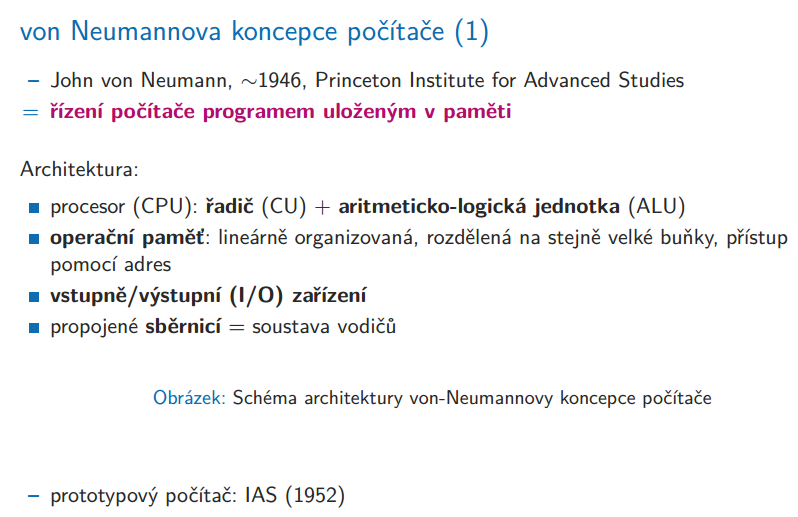
\includegraphics[scale=0.65]{img/prvni_odstavec/otazka1/von_neuman1.png}	
\end{figure}

\begin{figure} [h]
	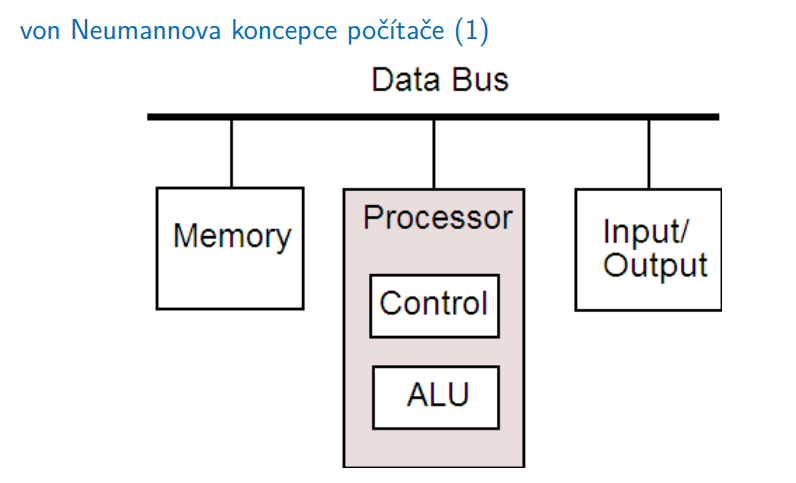
\includegraphics[scale=0.65]{img/prvni_odstavec/otazka1/von_neuman2.png}	
\end{figure}

\begin{figure} [h]
	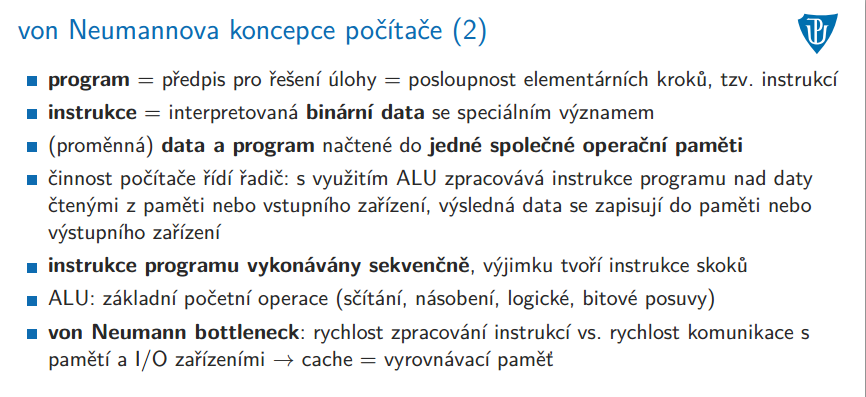
\includegraphics[scale=0.65]{img/prvni_odstavec/otazka1/von_neuman3.png}	
\end{figure}

\begin{figure} [h]
	
\includegraphics[scale=0.65]{img/prvni_odstavec/otazka1/von_neuman4.png}	
\end{figure}

\clearpage
\subsubsection{Harvardská architektura}
\begin{figure} [h]
	
\includegraphics[scale=0.65]{img/prvni_odstavec/otazka1/harvardska_koncepce.png}	
\end{figure}

%-----------------------------------otazka 2------------------------------------------

\clearpage
\subsection{Binární logika, logické operace a funkce, logické obvody}
\subsubsection{Binární logika}
\begin{figure} [h]
	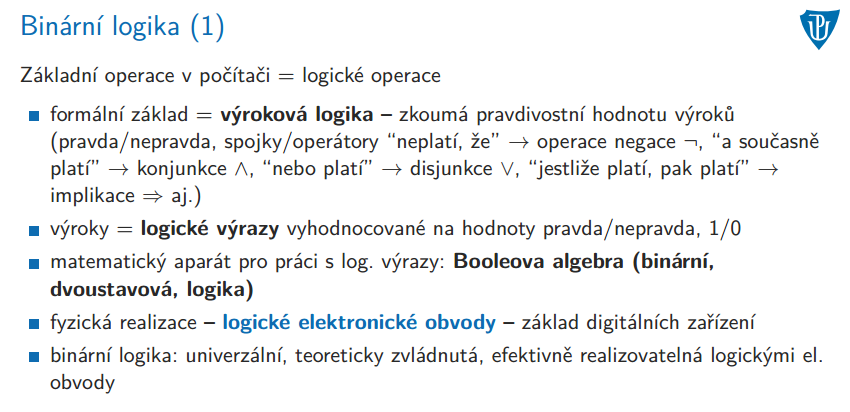
\includegraphics[scale=0.65]{img/prvni_odstavec/otazka2/binarni_logika1.png}	
\end{figure}

\begin{figure} [h]
	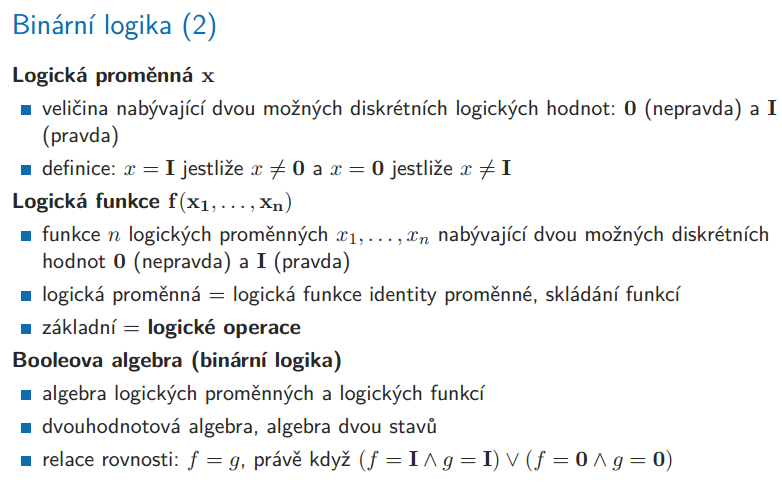
\includegraphics[scale=0.65]{img/prvni_odstavec/otazka2/binarni_logika2.png}	
\end{figure}

\clearpage
\subsubsection{Logické operace}
\begin{figure} [h]
	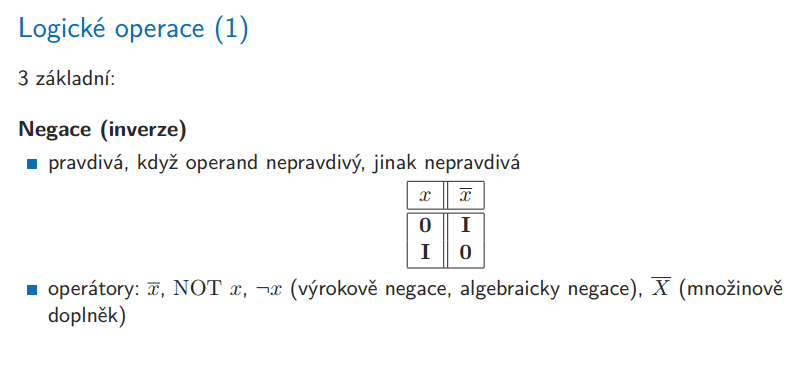
\includegraphics[scale=0.65]{img/prvni_odstavec/otazka2/logicke_operace1.png}	
\end{figure}

\begin{figure} [h]
	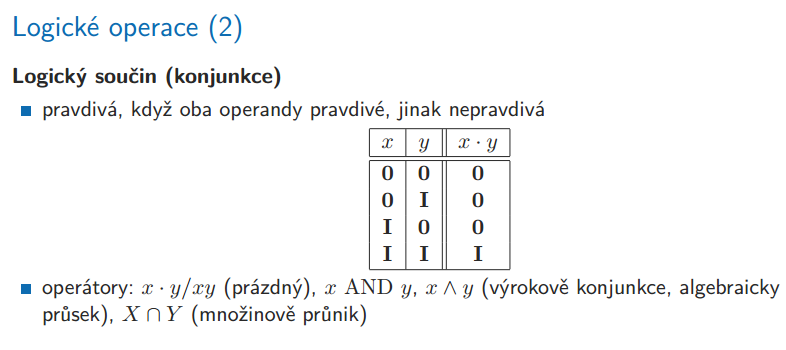
\includegraphics[scale=0.65]{img/prvni_odstavec/otazka2/logicke_operace2.png}	
\end{figure}

\begin{figure} [h]
	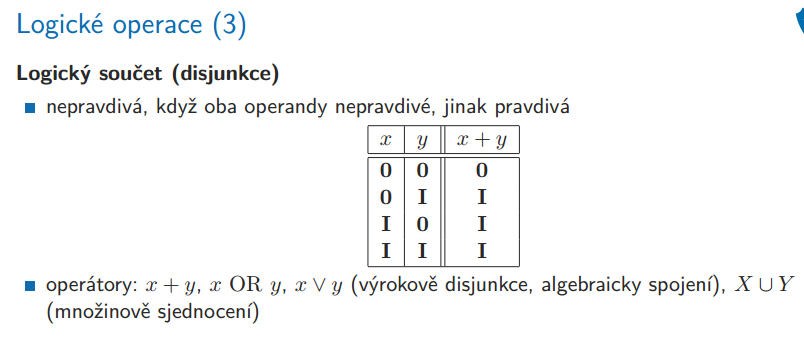
\includegraphics[scale=0.65]{img/prvni_odstavec/otazka2/logicke_operace3.png}	
\end{figure}

\begin{figure} [h]
	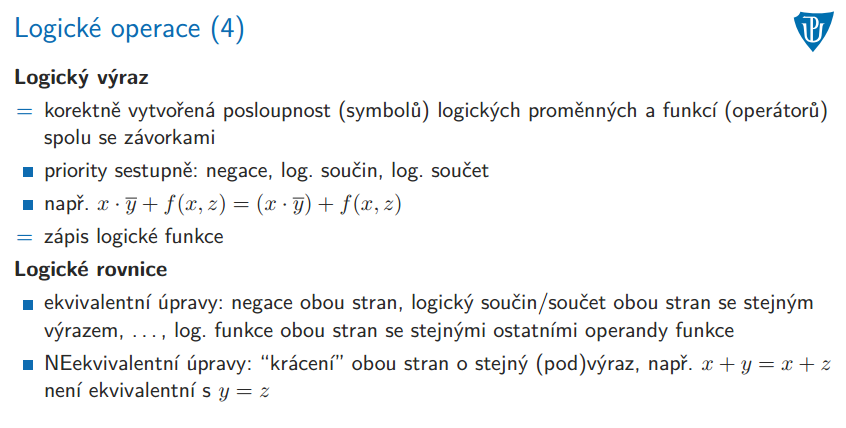
\includegraphics[scale=0.65]{img/prvni_odstavec/otazka2/logicke_operace4.png}	
\end{figure}

\begin{figure} [h]
	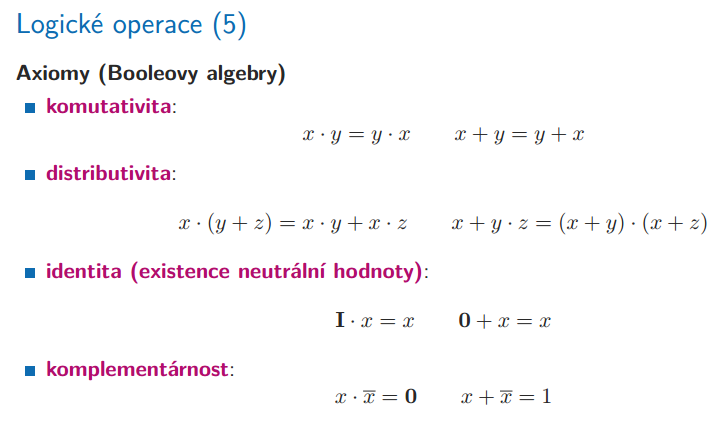
\includegraphics[scale=0.65]{img/prvni_odstavec/otazka2/logicke_operace5.png}	
\end{figure}

\begin{figure} [h]
	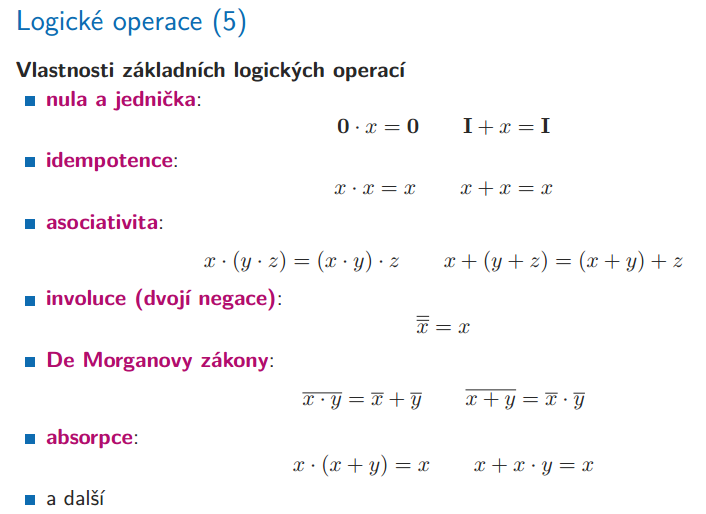
\includegraphics[scale=0.65]{img/prvni_odstavec/otazka2/logicke_operace6.png}	
\end{figure}

\begin{figure} [h]
	
\includegraphics[scale=0.65]{img/prvni_odstavec/otazka2/logicke_operace7.png}	
\end{figure}

\begin{figure} [h]
	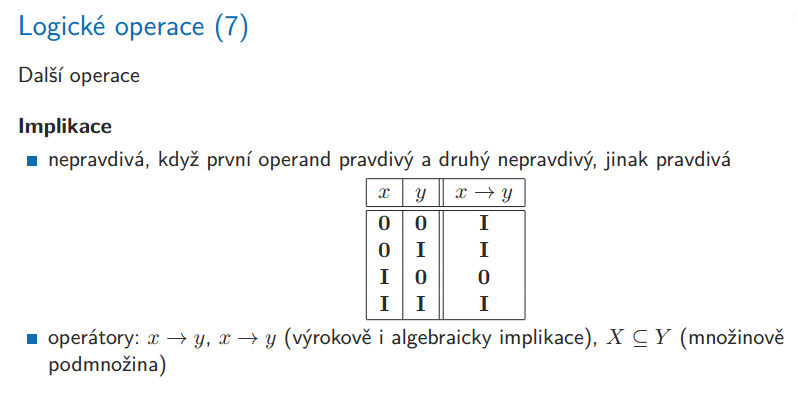
\includegraphics[scale=0.65]{img/prvni_odstavec/otazka2/logicke_operace8.png}	
\end{figure}

\begin{figure} [h]
	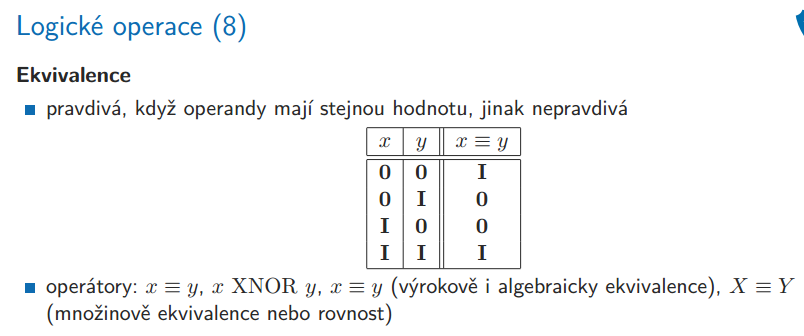
\includegraphics[scale=0.65]{img/prvni_odstavec/otazka2/logicke_operace9.png}	
\end{figure}

\begin{figure} [h]
	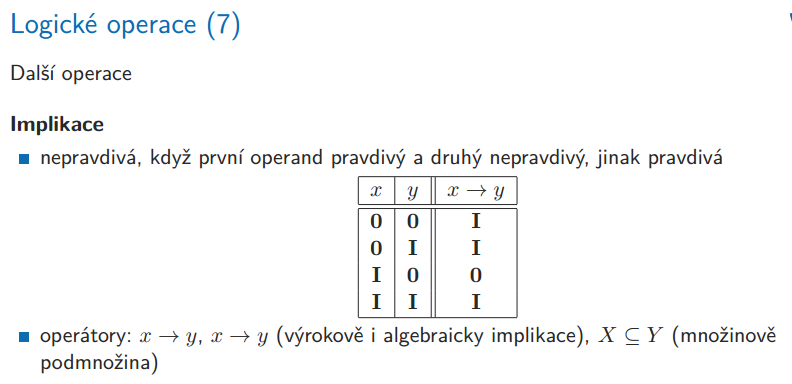
\includegraphics[scale=0.65]{img/prvni_odstavec/otazka2/logicke_operace10.png}	
\end{figure}

\begin{figure} [h]
	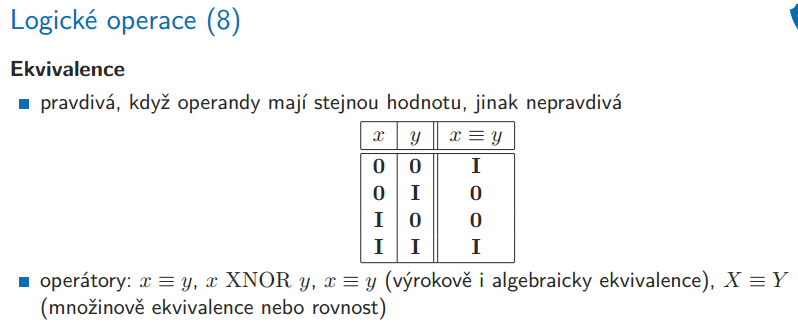
\includegraphics[scale=0.65]{img/prvni_odstavec/otazka2/logicke_operace11.png}	
\end{figure}

\begin{figure} [h]
	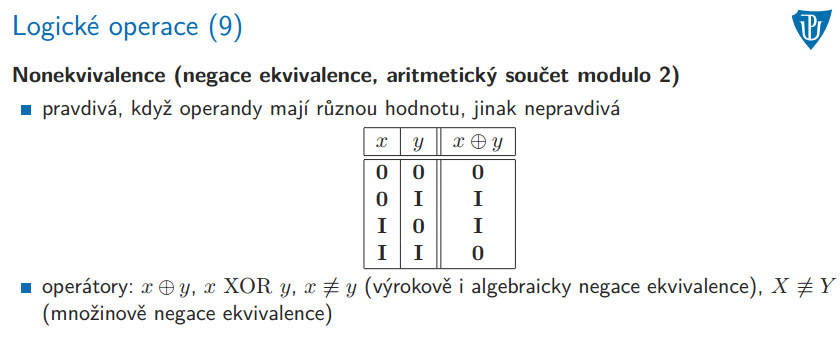
\includegraphics[scale=0.65]{img/prvni_odstavec/otazka2/logicke_operace12.png}	
\end{figure}

\begin{figure} [h]
	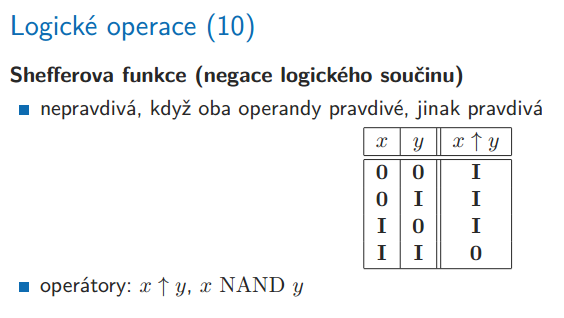
\includegraphics[scale=0.65]{img/prvni_odstavec/otazka2/logicke_operace13.png}	
\end{figure}

\begin{figure} [h]
	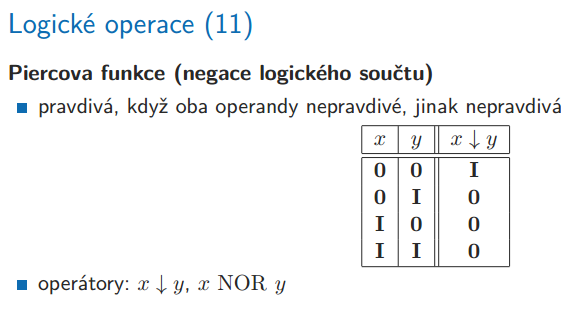
\includegraphics[scale=0.65]{img/prvni_odstavec/otazka2/logicke_operace14.png}	
\end{figure}

\clearpage
\subsubsection{Logické funkce}
\begin{figure} [h]
	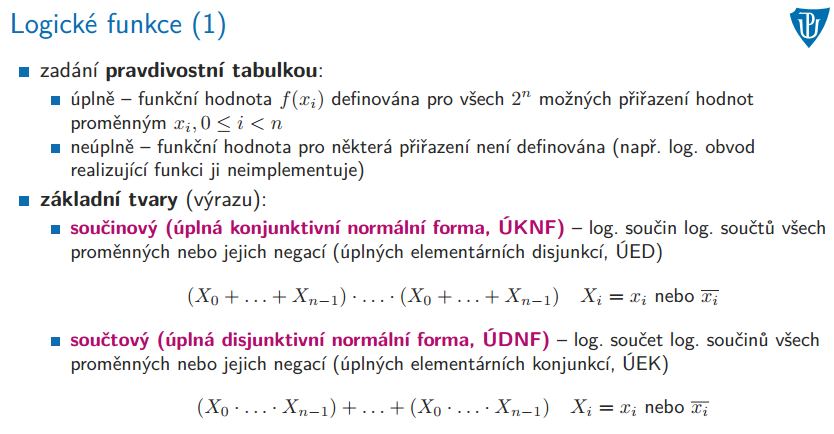
\includegraphics[scale=0.65]{img/prvni_odstavec/otazka2/logicke_funkce1.png}	
\end{figure}

\begin{figure} [h]
	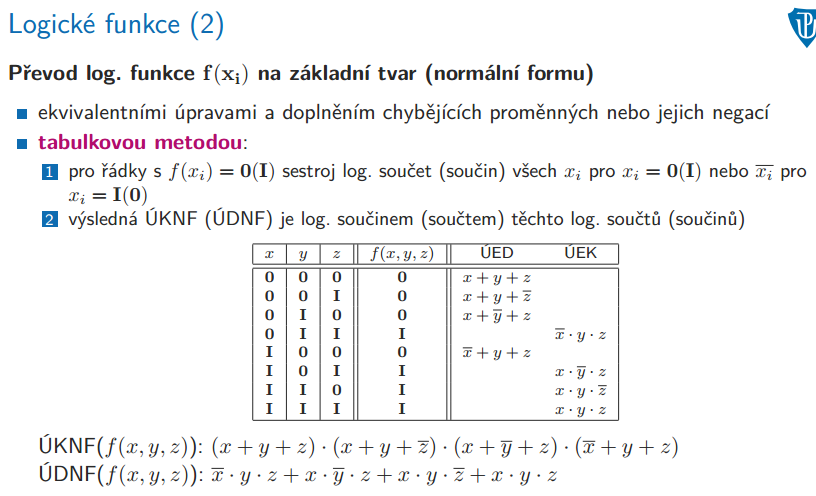
\includegraphics[scale=0.65]{img/prvni_odstavec/otazka2/logicke_funkce2.png}	
\end{figure}

\begin{figure} [h]
	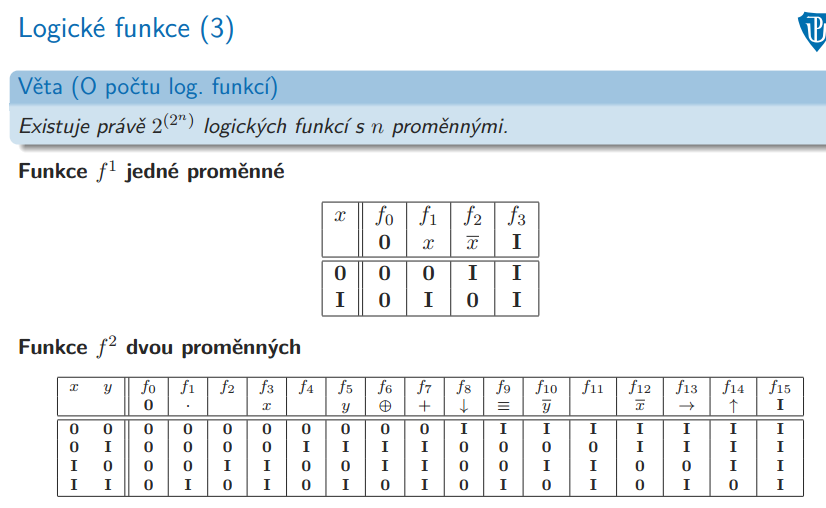
\includegraphics[scale=0.65]{img/prvni_odstavec/otazka2/logicke_funkce3.png}	
\end{figure}

\begin{figure} [h]
	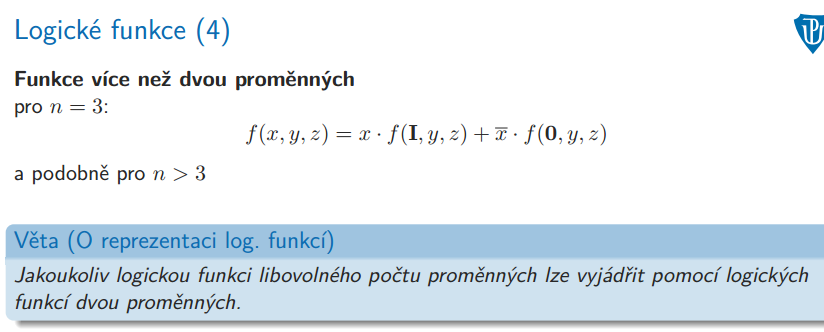
\includegraphics[scale=0.65]{img/prvni_odstavec/otazka2/logicke_funkce4.png}	
\end{figure}

\begin{figure} [h]
	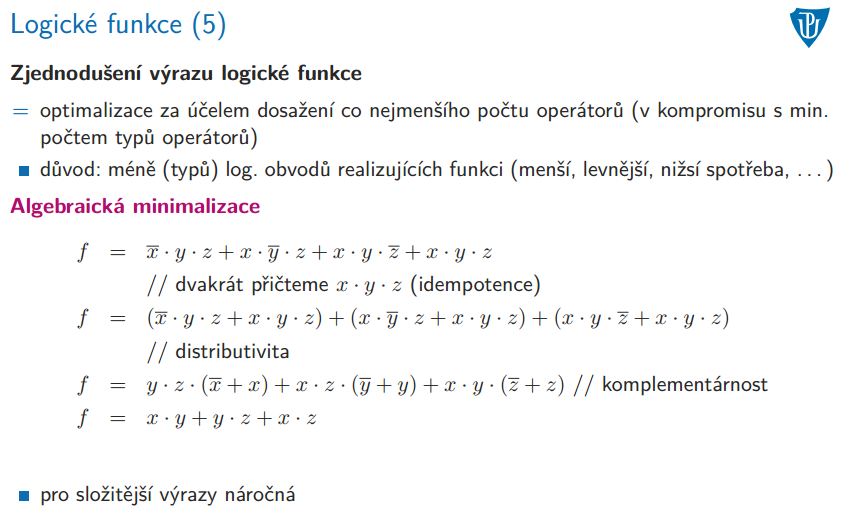
\includegraphics[scale=0.65]{img/prvni_odstavec/otazka2/logicke_funkce5.png}	
\end{figure}

\begin{figure} [h]
	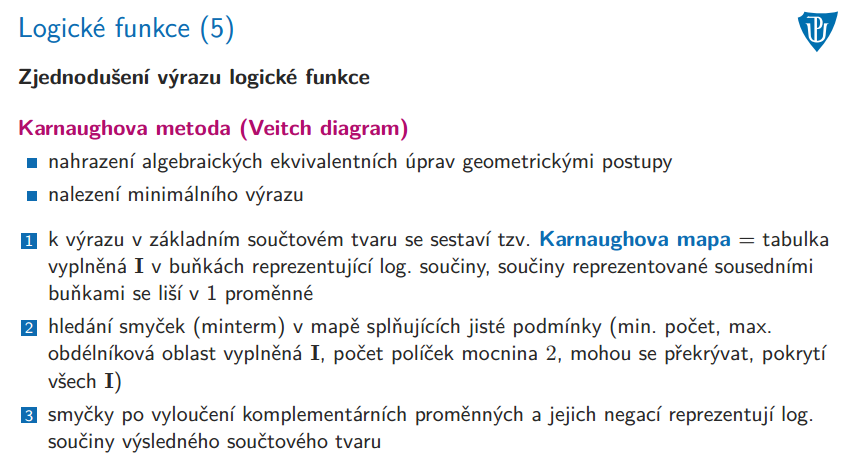
\includegraphics[scale=0.65]{img/prvni_odstavec/otazka2/logicke_funkce6.png}	
\end{figure}

\begin{figure} [h]
	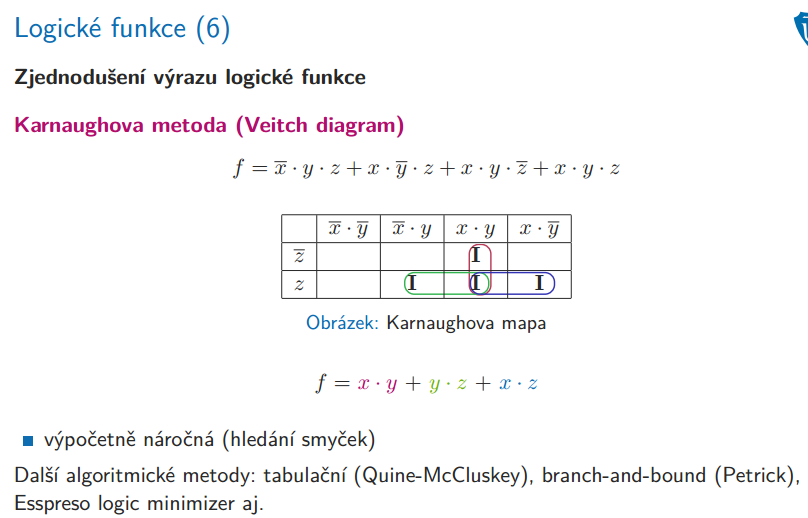
\includegraphics[scale=0.65]{img/prvni_odstavec/otazka2/logicke_funkce7.png}	
\end{figure}

\begin{figure} [h]
	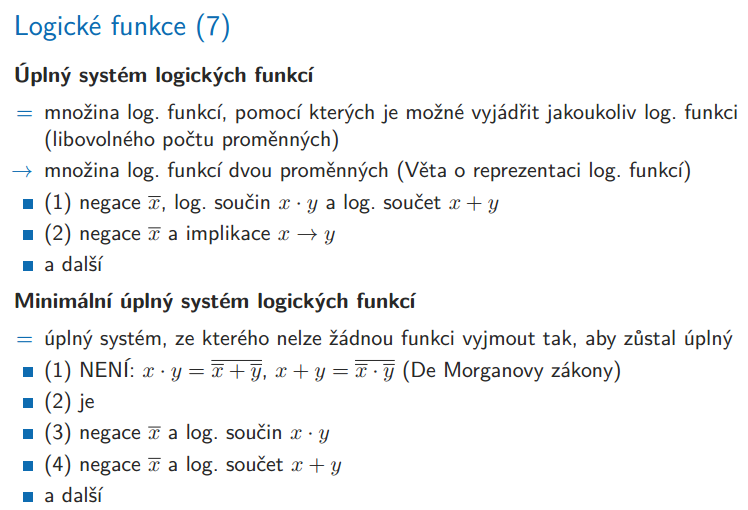
\includegraphics[scale=0.65]{img/prvni_odstavec/otazka2/logicke_funkce8.png}	
\end{figure}

\begin{figure} [h]
	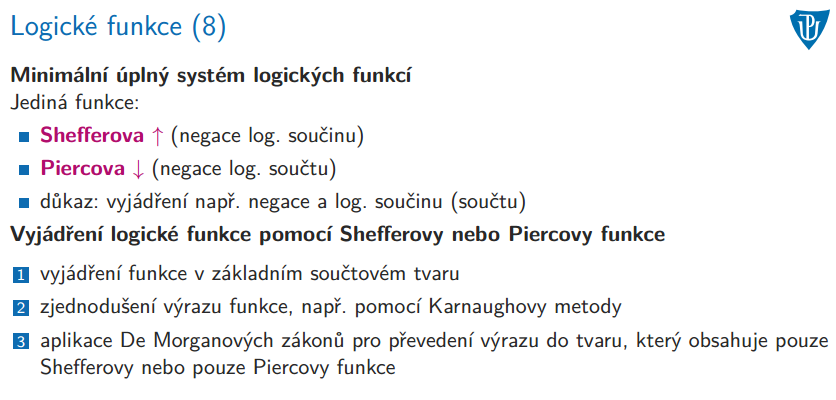
\includegraphics[scale=0.65]{img/prvni_odstavec/otazka2/logicke_funkce9.png}	
\end{figure}


\clearpage
\subsubsection{Logické obvody}
\begin{figure} [h]
	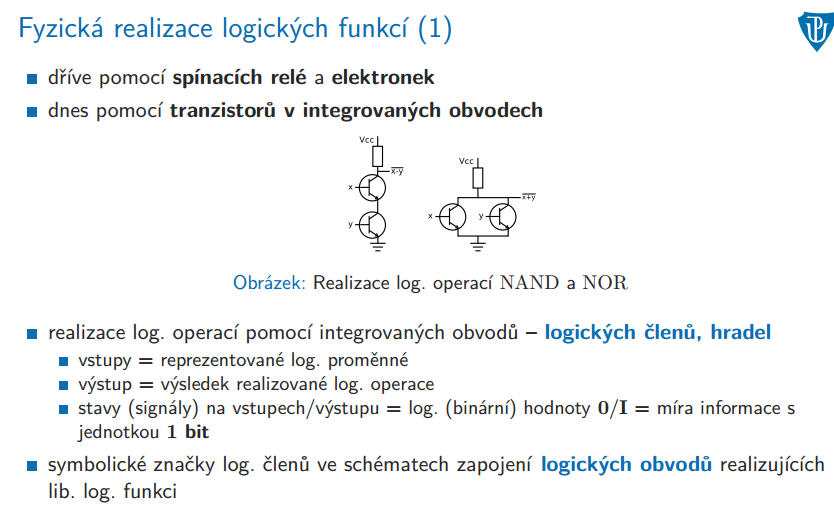
\includegraphics[scale=0.65]{img/prvni_odstavec/otazka2/fyzicka_realizace_logickych_funkci1.png}	
\end{figure}

\begin{figure} [h]
	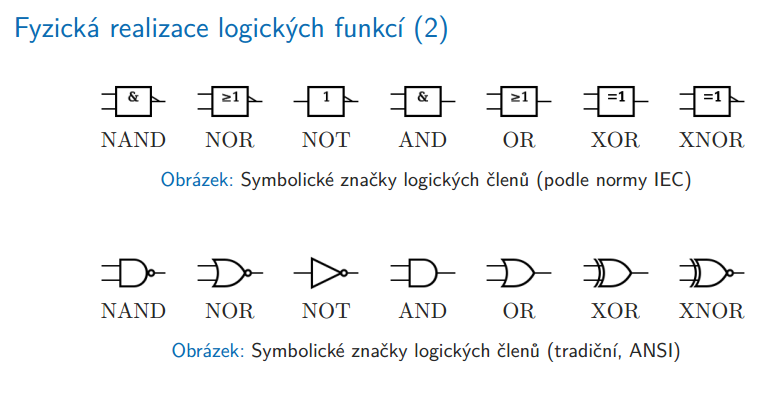
\includegraphics[scale=0.65]{img/prvni_odstavec/otazka2/fyzicka_realizace_logickych_funkci2.png}	
\end{figure}

\begin{figure} [h]
	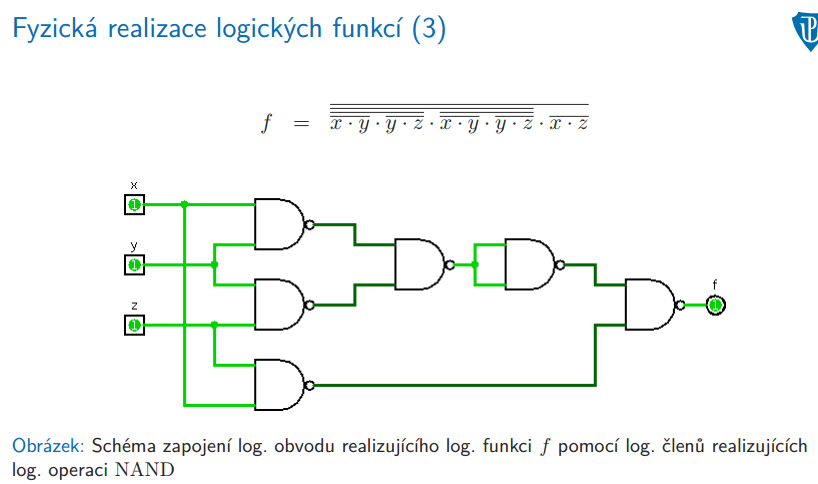
\includegraphics[scale=0.65]{img/prvni_odstavec/otazka2/fyzicka_realizace_logickych_funkci3.png}	
\end{figure}

\begin{figure} [h]
	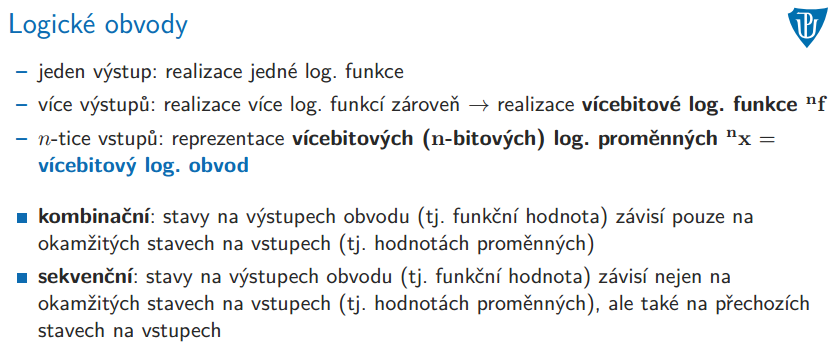
\includegraphics[scale=0.65]{img/prvni_odstavec/otazka2/logicke_obvody.png}	
\end{figure}

\begin{figure} [h]
	
\includegraphics[scale=0.65]{img/prvni_odstavec/otazka2/kombinacni_logicke_obvody1.png}	
\end{figure}

\begin{figure} [h]
	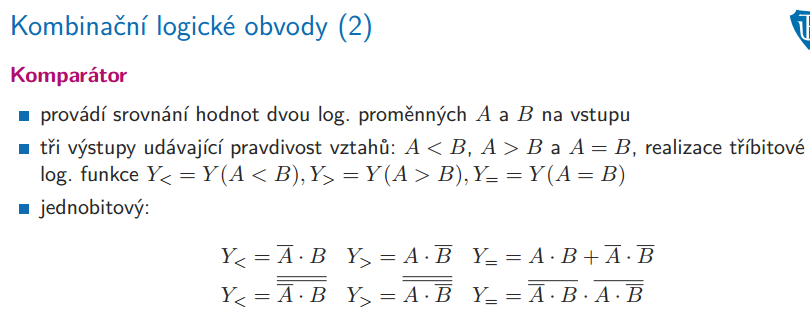
\includegraphics[scale=0.65]{img/prvni_odstavec/otazka2/kombinacni_logicke_obvody2.png}	
\end{figure}

\begin{figure} [h]
	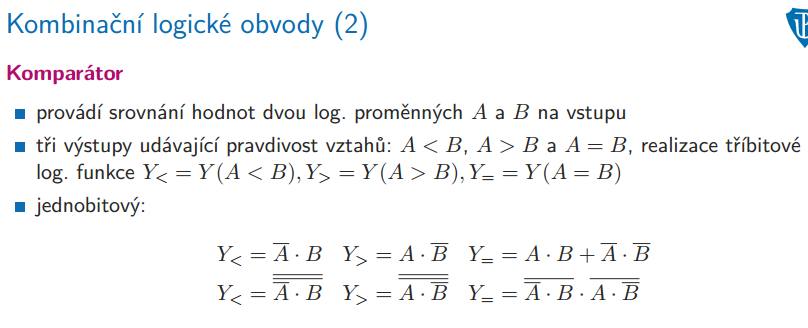
\includegraphics[scale=0.65]{img/prvni_odstavec/otazka2/kombinacni_logicke_obvody3.png}	
\end{figure}

\begin{figure} [h]
	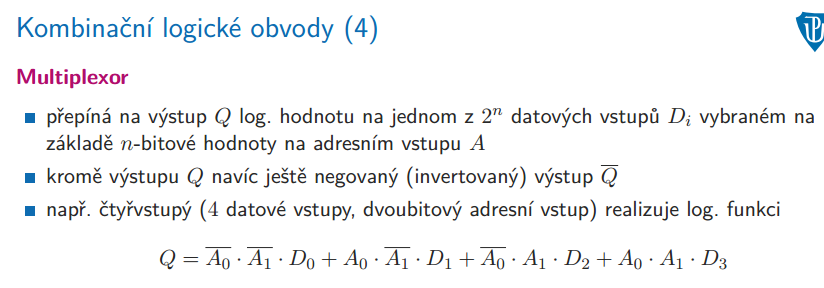
\includegraphics[scale=0.65]{img/prvni_odstavec/otazka2/kombinacni_logicke_obvody4.png}	
\end{figure}

\begin{figure} [h]
	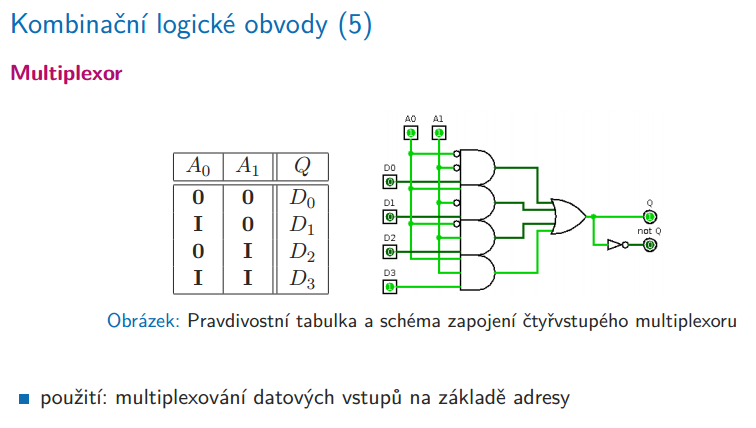
\includegraphics[scale=0.65]{img/prvni_odstavec/otazka2/kombinacni_logicke_obvody5.png}	
\end{figure}

\begin{figure} [h]
	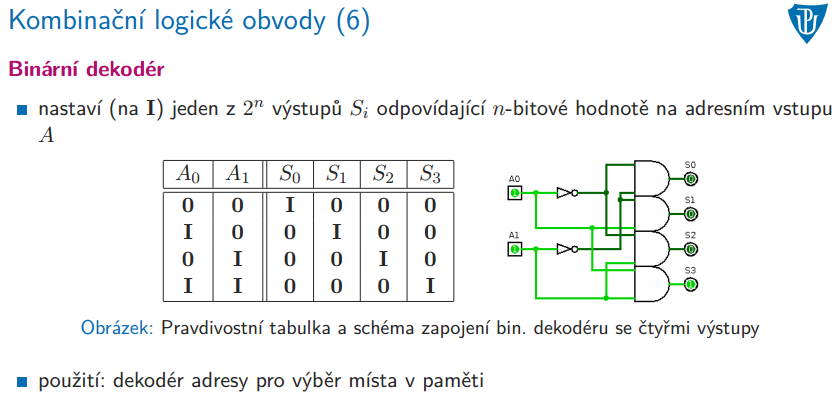
\includegraphics[scale=0.65]{img/prvni_odstavec/otazka2/kombinacni_logicke_obvody6.png}	
\end{figure}

\begin{figure} [h]
	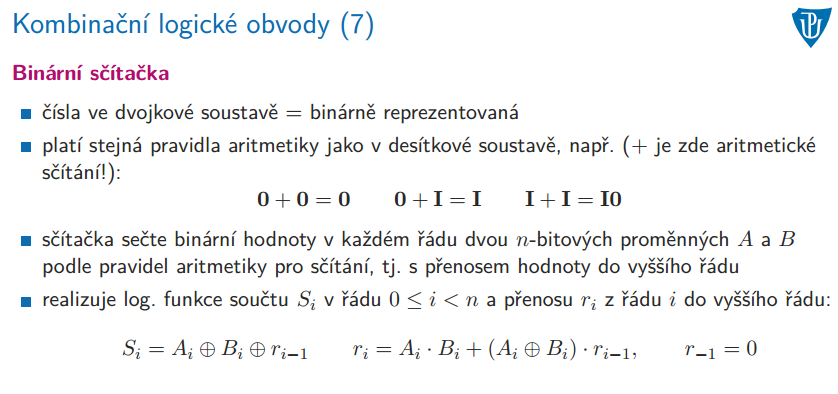
\includegraphics[scale=0.65]{img/prvni_odstavec/otazka2/kombinacni_logicke_obvody7.png}	
\end{figure}

\begin{figure} [h]
	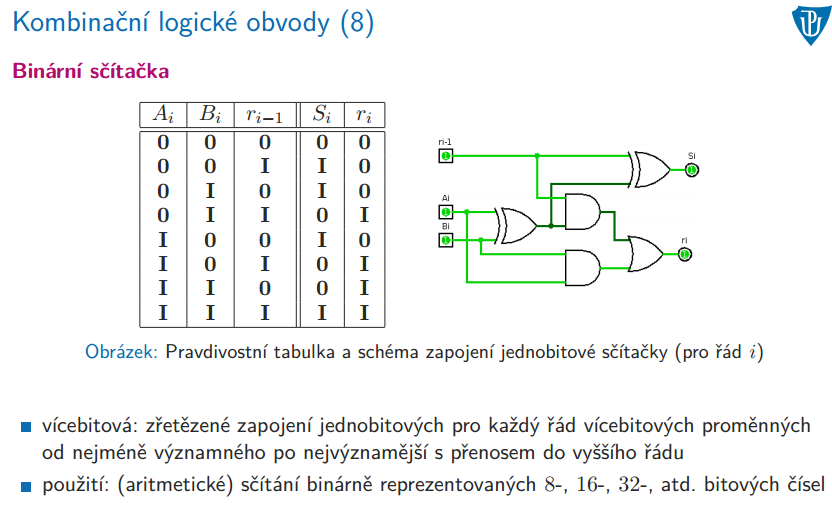
\includegraphics[scale=0.65]{img/prvni_odstavec/otazka2/kombinacni_logicke_obvody8.png}	
\end{figure}

\begin{figure} [h]
	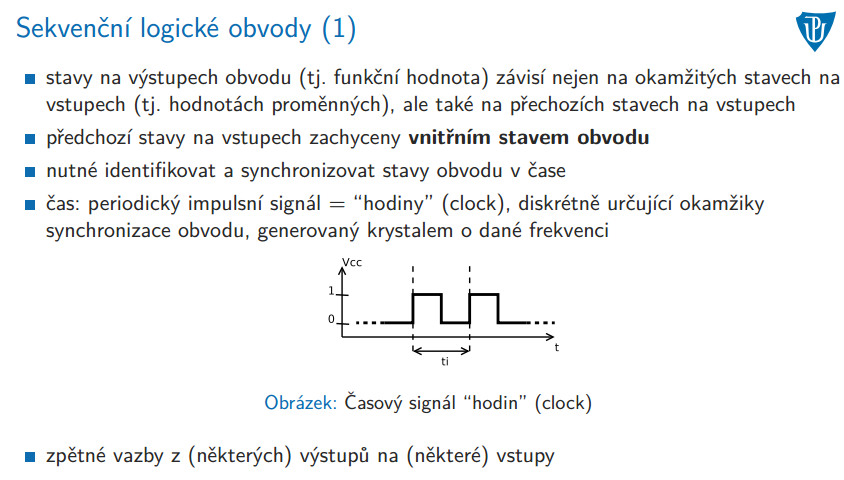
\includegraphics[scale=0.65]{img/prvni_odstavec/otazka2/sekvencni_logicke_obvody1.png}	
\end{figure}

\begin{figure} [h]
	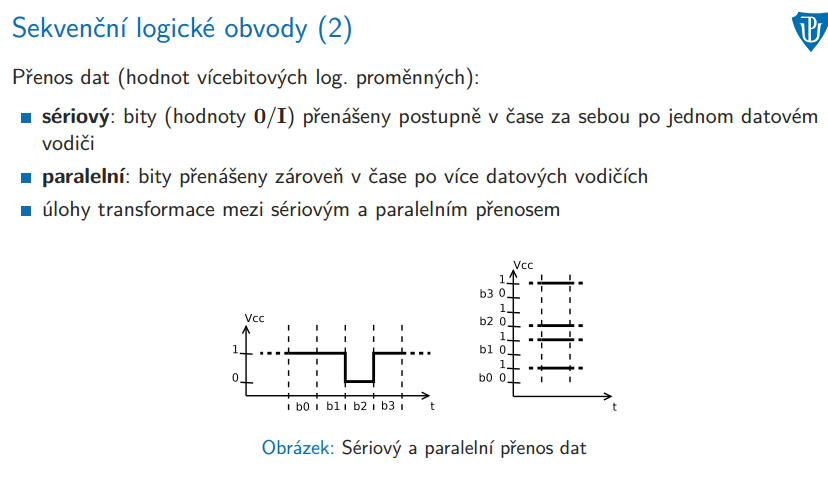
\includegraphics[scale=0.65]{img/prvni_odstavec/otazka2/sekvencni_logicke_obvody2.png}	
\end{figure}

\begin{figure} [h]
	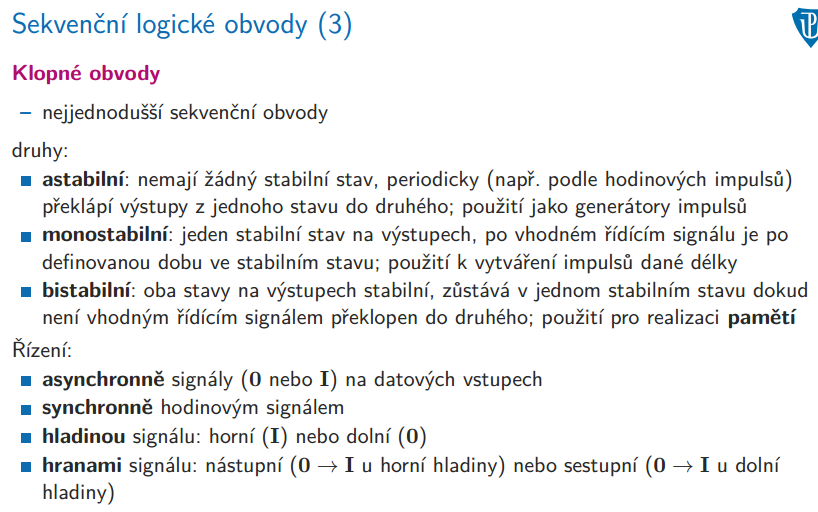
\includegraphics[scale=0.65]{img/prvni_odstavec/otazka2/sekvencni_logicke_obvody3.png}	
\end{figure}

\begin{figure} [h]
	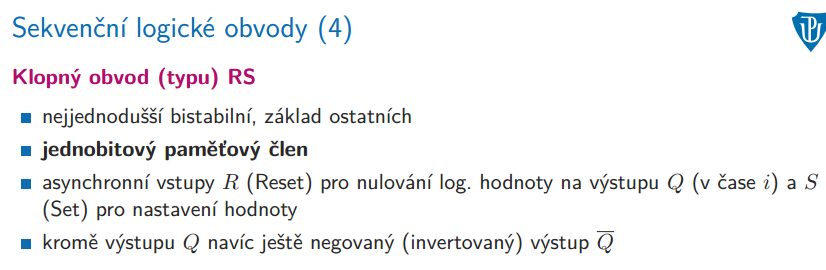
\includegraphics[scale=0.65]{img/prvni_odstavec/otazka2/sekvencni_logicke_obvody4.png}	
\end{figure}

\begin{figure} [h]
	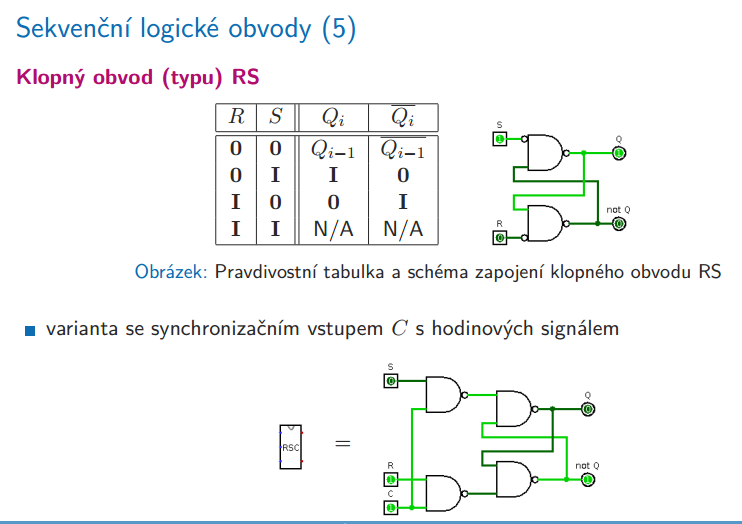
\includegraphics[scale=0.65]{img/prvni_odstavec/otazka2/sekvencni_logicke_obvody5.png}	
\end{figure}

\begin{figure} [h]
	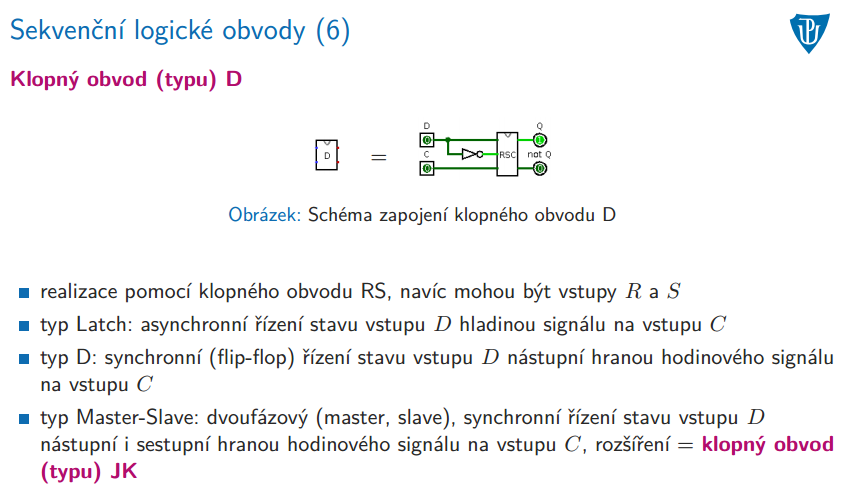
\includegraphics[scale=0.65]{img/prvni_odstavec/otazka2/sekvencni_logicke_obvody6.png}	
\end{figure}

\clearpage
\begin{figure} [h]
	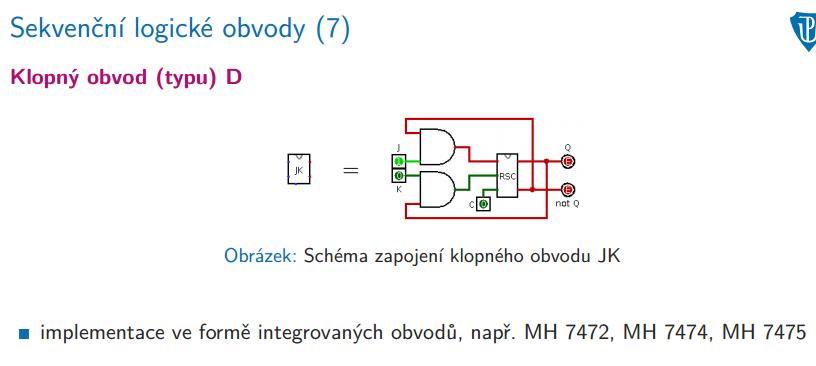
\includegraphics[scale=0.65]{img/prvni_odstavec/otazka2/sekvencni_logicke_obvody7.png}	
\end{figure}

\begin{figure} [h]
	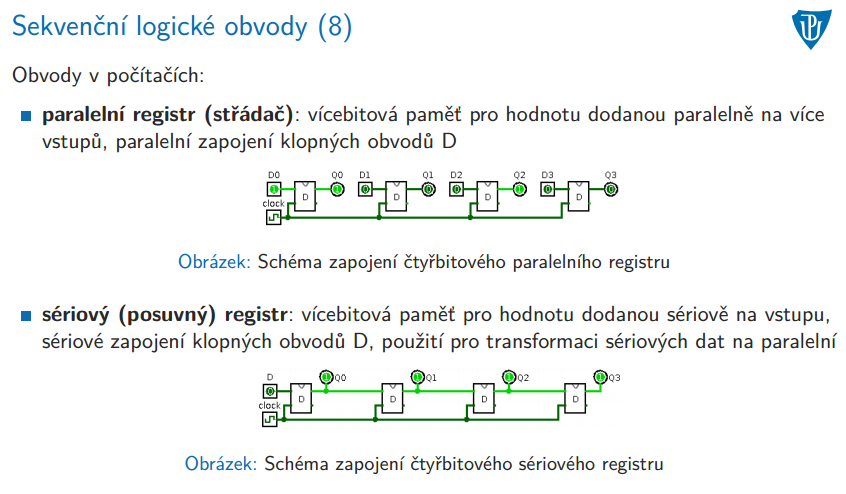
\includegraphics[scale=0.65]{img/prvni_odstavec/otazka2/sekvencni_logicke_obvody8.png}	
\end{figure}

\begin{figure} [h]
	\includegraphics[scale=0.65]{img/prvni_odstavec/otazka2/sekvencni_logicke_obvody9.png}	
\end{figure}


%-----------------------------------otazka 3------------------------------------------

\clearpage
\subsection{Reprezentace čísel a znaků v paměti počítače}
\begin{figure} [h]
	\includegraphics[scale=0.65]{img/prvni_odstavec/otazka3/kodovani_cisel.png}	
\end{figure}

\clearpage
\subsubsection{Reprezentace čísel}

\begin{figure} [h]
	\includegraphics[scale=0.65]{img/prvni_odstavec/otazka3/cela_cisla1.png}	
\end{figure}

\begin{figure} [h]
	\includegraphics[scale=0.65]{img/prvni_odstavec/otazka3/cela_cisla2.png}	
\end{figure}

\begin{figure} [h]
	\includegraphics[scale=0.65]{img/prvni_odstavec/otazka3/cela_cisla3.png}	
\end{figure}

\begin{figure} [h]
	\includegraphics[scale=0.65]{img/prvni_odstavec/otazka3/cisla_s_radovou_carkou1.png}	
\end{figure}

\begin{figure} [h]
	\includegraphics[scale=0.65]{img/prvni_odstavec/otazka3/cisla_s_radovou_carkou2.png}	
\end{figure}

\begin{figure} [h]
	\includegraphics[scale=0.65]{img/prvni_odstavec/otazka3/cisla_s_radovou_carkou3.png}	
\end{figure}

\begin{figure} [h]
	\includegraphics[scale=0.65]{img/prvni_odstavec/otazka3/cisla_s_radovou_carkou4.png}	
\end{figure}

\begin{figure} [h]
	\includegraphics[scale=0.65]{img/prvni_odstavec/otazka3/cisla_s_radovou_carkou5.png}	
\end{figure}

\begin{figure} [h]
	\includegraphics[scale=0.65]{img/prvni_odstavec/otazka3/cisla_s_radovou_carkou6.png}	
\end{figure}

\begin{figure} [h]
	\includegraphics[scale=0.65]{img/prvni_odstavec/otazka3/cisla_s_radovou_carkou7.png}	
\end{figure}

\begin{figure} [h]
	\includegraphics[scale=0.65]{img/prvni_odstavec/otazka3/cisla_s_radovou_carkou8.png}	
\end{figure}

\begin{figure} [h]
	\includegraphics[scale=0.65]{img/prvni_odstavec/otazka3/text1.png}	
\end{figure}

\begin{figure} [h]
	\includegraphics[scale=0.65]{img/prvni_odstavec/otazka3/text2.png}	
\end{figure}

\begin{figure} [h]
	\includegraphics[scale=0.65]{img/prvni_odstavec/otazka3/text3.png}	
\end{figure}

\begin{figure} [h]
	\includegraphics[scale=0.65]{img/prvni_odstavec/otazka3/text4.png}	
\end{figure}

\begin{figure} [h]
	\includegraphics[scale=0.65]{img/prvni_odstavec/otazka3/text5.png}	
\end{figure}

\begin{figure} [h]
	\includegraphics[scale=0.65]{img/prvni_odstavec/otazka3/text6.png}	
\end{figure}

\begin{figure} [h]
	\includegraphics[scale=0.65]{img/prvni_odstavec/otazka3/text7.png}	
\end{figure}

\clearpage
\begin{figure} [h]
	\includegraphics[scale=0.65]{img/prvni_odstavec/otazka3/text8.png}	
\end{figure}

\begin{figure} [h]
	\includegraphics[scale=0.65]{img/prvni_odstavec/otazka3/text9.png}	
\end{figure}

\begin{figure} [h]
	\includegraphics[scale=0.65]{img/prvni_odstavec/otazka3/text10.png}	
\end{figure}

\begin{figure} [h]
	\includegraphics[scale=0.65]{img/prvni_odstavec/otazka3/text11.png}	
\end{figure}


%-----------------------------------otazka 4------------------------------------------

\clearpage
\subsection{Osobní počítač (PC), základní deska, chipset a sběrnice (interní, externí)}
\subsubsection{Osobní počítač (PC)}
\begin{figure} [h]
	\includegraphics[scale=0.65]{img/prvni_odstavec/otazka4/osobni_pocitac.png}	
\end{figure}

\begin{figure} [h]
	\includegraphics[scale=0.65]{img/prvni_odstavec/otazka4/pocitacova_sestava.png}	
\end{figure}

\begin{figure} [h]
	\includegraphics[scale=0.65]{img/prvni_odstavec/otazka4/soucasti_pocitace1.png}	
\end{figure}

\begin{figure} [h]
	\includegraphics[scale=0.65]{img/prvni_odstavec/otazka4/soucasti_pocitace2.png}	
\end{figure}

\begin{figure} [h]
	\includegraphics[scale=0.65]{img/prvni_odstavec/otazka4/soucasti_pocitace3.png}	
\end{figure}

\clearpage
\subsubsection{Základní deska}
\begin{figure} [h]
	\includegraphics[scale=0.65]{img/prvni_odstavec/otazka4/zakladni_deska1.png}	
\end{figure}

\begin{figure} [h]
	\includegraphics[scale=0.65]{img/prvni_odstavec/otazka4/zakladni_deska2.png}	
\end{figure}

\begin{figure} [h]
	\includegraphics[scale=0.65]{img/prvni_odstavec/otazka4/zakladni_deska3.png}	
\end{figure}

\begin{figure} [h]
	\includegraphics[scale=0.65]{img/prvni_odstavec/otazka4/zakladni_deska4.png}	
\end{figure}

\begin{figure} [h]
	\includegraphics[scale=0.65]{img/prvni_odstavec/otazka4/zakladni_deska5.png}	
\end{figure}

\begin{figure} [h]
	\includegraphics[scale=0.65]{img/prvni_odstavec/otazka4/zakladni_deska6.png}	
\end{figure}

\begin{figure} [h]
	\includegraphics[scale=0.65]{img/prvni_odstavec/otazka4/zakladni_deska7.png}	
\end{figure}

\begin{figure} [h]
	\includegraphics[scale=0.65]{img/prvni_odstavec/otazka4/zakladni_deska8.png}	
\end{figure}

\begin{figure} [h]
	\includegraphics[scale=0.65]{img/prvni_odstavec/otazka4/zakladni_deska9.png}	
\end{figure}

\begin{figure} [h]
	\includegraphics[scale=0.65]{img/prvni_odstavec/otazka4/zakladni_deska10.png}	
\end{figure}

\begin{figure} [h]
	\includegraphics[scale=0.65]{img/prvni_odstavec/otazka4/zakladni_deska11.png}	
\end{figure}

\begin{figure} [h]
	\includegraphics[scale=0.65]{img/prvni_odstavec/otazka4/zakladni_deska12.png}	
\end{figure}


\clearpage
\subsubsection{Chipset a sběrnice (interní, externí)}
\begin{figure} [h]
	\includegraphics[scale=0.65]{img/prvni_odstavec/otazka4/cipova_sada1.png}	
\end{figure}

\begin{figure} [h]
	\includegraphics[scale=0.65]{img/prvni_odstavec/otazka4/cipova_sada2.png}	
\end{figure}

\begin{figure} [h]
	\includegraphics[scale=0.65]{img/prvni_odstavec/otazka4/cipova_sada3.png}	
\end{figure}

\begin{figure} [h]
	\includegraphics[scale=0.65]{img/prvni_odstavec/otazka4/rozhrani_vnitrni1.png}	
\end{figure}

\begin{figure} [h]
	\includegraphics[scale=0.65]{img/prvni_odstavec/otazka4/rozhrani_vnitrni2.png}	
\end{figure}

\begin{figure} [h]
	\includegraphics[scale=0.65]{img/prvni_odstavec/otazka4/rozhrani_vnitrni3.png}	
\end{figure}

\begin{figure} [h]
	\includegraphics[scale=0.65]{img/prvni_odstavec/otazka4/rozhrani_vnitrni4.png}	
\end{figure}

\begin{figure} [h]
	\includegraphics[scale=0.65]{img/prvni_odstavec/otazka4/rozhrani_vnitrni5.png}	
\end{figure}

\begin{figure} [h]
	\includegraphics[scale=0.65]{img/prvni_odstavec/otazka4/rozhrani_vnejsi1.png}	
\end{figure}

\begin{figure} [h]
	\includegraphics[scale=0.65]{img/prvni_odstavec/otazka4/rozhrani_vnejsi2.png}	
\end{figure}

\begin{figure} [h]
	\includegraphics[scale=0.65]{img/prvni_odstavec/otazka4/rozhrani_vnejsi3.png}	
\end{figure}

\begin{figure} [h]
	\includegraphics[scale=0.65]{img/prvni_odstavec/otazka4/rozhrani_vnejsi4.png}	
\end{figure}

\begin{figure} [h]
	\includegraphics[scale=0.65]{img/prvni_odstavec/otazka4/rozhrani_vnejsi5.png}	
\end{figure}

\begin{figure} [h]
	\includegraphics[scale=0.65]{img/prvni_odstavec/otazka4/rozhrani_vnejsi6.png}	
\end{figure}

\begin{figure} [h]
	\includegraphics[scale=0.65]{img/prvni_odstavec/otazka4/rozhrani_vnejsi7.png}	
\end{figure}


%-----------------------------------otazka 5------------------------------------------

\clearpage
\subsection{Procesor (CPU), vykonávání instrukcí, podprogramy a zásobník, přerušení}
\subsubsection{Procesor}
\begin{comment}
\begin{itemize}
	\item základní součást počítače (mozek počítače)
	\item integrovaný obvod, provádějící strojové instrukce, ze kterých je složen počítačový program umístěný v operační paměti počítače
\end{itemize}

\textbf{OBECNÁ STRUKTURA CPU}
\begin{itemize}
	\item Je to jednotka, která zpracovává instrukce
	\item Aritmeticko-logická jednotka (ALU) - provádí výpočty
	\item Řídící jednotka - řídí chod CPU
	\item Registry - slouží k uchování právě zpracovávaných dat (násobně rychlejší přístup než do paměti)
\end{itemize}

\textbf{INSTRUKČNÍ SADA}
\begin{itemize}
	\item Sada ovládající procesor (specifikovaná pro daný CPU/rodinu CPU)
	\item Instrukce a jejich operandy jsou reprezentovány jako čísla - strojový kód
	\item Každá instrukce má obvykle 0 až 3 operandy (může to být registr, konstantu nebo místo v paměti)
	\item Pro snazší porozumění, se instrukce CPU zapisují v jazyce symbolických adres (též vulgárně označován jako Assembler)
	\item Instrukce jsou zpracovávány (z důvodu větší efektivity) v několika krocích:
	\begin{enumerate}
		\item načtení instrukce do CPU (Fetch)
		\item dekódování instrukce (decode)
		\item výpočet adres operandů
		\item přesun operandů do CPU
		\item provedení operace (Execute)
		\item uložení výsledku (Write-back)
	\end{enumerate}
	\item Pipelining - umožňuje zvýšit efektivitu CPU (díky rozdělení do jednotlivých kroků je možné provádět více instrukcí zároveň)
	\item Superskalární procesor - procesor může mít víc jednotek např. pro výpočty (FPU, ALU), musíme se postarat o správnou synchronizaci
	\item Problém s podmíněnými skoky (branch prediction) - jakmile se má provést nějaký podmíněný, nevíme, která instrukce bude následovat -> může se stát, že se musí vyprázdnit instrukci z pipeline -> zpomalení
\end{itemize}

\begin{figure} [h]
		\includegraphics[scale=0.7]{img/pipelining.png}
		\caption{pipelining}	
\end{figure}
\end{comment}

\begin{figure} [h]
	\includegraphics[scale=0.65]{img/prvni_odstavec/otazka5/procesor1.png}	
\end{figure}

\begin{figure} [h]
	\includegraphics[scale=0.65]{img/prvni_odstavec/otazka5/procesor2.png}	
\end{figure}

\begin{figure} [h]
	\includegraphics[scale=0.65]{img/prvni_odstavec/otazka5/procesor3.png}	
\end{figure}

\begin{figure} [h]
	\includegraphics[scale=0.65]{img/prvni_odstavec/otazka5/procesor4.png}	
\end{figure}

\begin{figure} [h]
	\includegraphics[scale=0.65]{img/prvni_odstavec/otazka5/procesor5.png}	
\end{figure}

\begin{figure} [h]
	\includegraphics[scale=0.65]{img/prvni_odstavec/otazka5/procesor6.png}	
\end{figure}

\begin{figure} [h]
	\includegraphics[scale=0.65]{img/prvni_odstavec/otazka5/procesor7.png}	
\end{figure}

\begin{figure} [h]
	\includegraphics[scale=0.65]{img/prvni_odstavec/otazka5/procesor8.png}	
\end{figure}

\begin{figure} [h]
	\includegraphics[scale=0.65]{img/prvni_odstavec/otazka5/procesor9.png}	
\end{figure}

\clearpage
\subsubsection{Vykonávání instrukcí}
\begin{figure} [h]
	\includegraphics[scale=0.65]{img/prvni_odstavec/otazka5/vykonavani_instrukci1.png}	
\end{figure}

\begin{figure} [h]
	\includegraphics[scale=0.65]{img/prvni_odstavec/otazka5/vykonavani_instrukci2.png}	
\end{figure}

\clearpage
\subsubsection{Zásobník}
\begin{figure} [h]
	\includegraphics[scale=0.65]{img/prvni_odstavec/otazka5/zasobnik.png}	
\end{figure}

\clearpage
\subsubsection{Podprogramy}
\begin{figure} [h]
	\includegraphics[scale=0.65]{img/prvni_odstavec/otazka5/podprogramy1.png}	
\end{figure}

\begin{figure} [h]
	\includegraphics[scale=0.65]{img/prvni_odstavec/otazka5/podprogramy2.png}	
\end{figure}

\begin{figure} [h]
	\includegraphics[scale=0.65]{img/prvni_odstavec/otazka5/podprogramy3.png}	
\end{figure}

\begin{figure} [h]
	\includegraphics[scale=0.65]{img/prvni_odstavec/otazka5/podprogramy4.png}	
\end{figure}

\begin{figure} [h]
	\includegraphics[scale=0.65]{img/prvni_odstavec/otazka5/podprogramy5.png}	
\end{figure}

\begin{figure} [h]
	\includegraphics[scale=0.65]{img/prvni_odstavec/otazka5/podprogramy6.png}	
\end{figure}

\clearpage
\begin{figure} [h]
	\includegraphics[scale=0.65]{img/prvni_odstavec/otazka5/podprogramy7.png}	
\end{figure}

\clearpage
\subsubsection{Přerušení}
\begin{figure} [h]
	\includegraphics[scale=0.65]{img/prvni_odstavec/otazka5/preruseni1.png}	
\end{figure}

\begin{figure} [h]
	\includegraphics[scale=0.65]{img/prvni_odstavec/otazka5/preruseni2.png}	
\end{figure}

%-----------------------------------otazka 6------------------------------------------

\clearpage
\subsection{Paměti počítače (RAM, cache, disk, diskové pole)}

\subsubsection{Operační paměť (RAM)}
\begin{comment}
\begin{itemize}
	\item zásadní část počítače
	\item uložení kódu a dat běžících v OS
	\item přístup k zařízením (DMA) - Direct Memory Access - přístup zařízení se namapuje do
operační paměti a dá se poté přistupovat k zařízení přes operační paměť
	\item virtualní paměť umožňuje například přístup k souborovému systému
	\item z HW pohledu může byt operační paměť realizovaná různými způsoby (DRAM, SRAM,
(EEP)ROM, ale i HDD, SSD, flash paměti)
	\item přístup k CPU k paměti nemusí být přímočarý (L1, L2 a L3 cache)
	\item pro jednoduchost budeme HW stránku věci zanedbávat
\end{itemize}

\textbf{POŽADAVKY NA OPERAČNÍ PAMĚŤ}
\begin{itemize}
	\item evidence prostoru volného a přiděleného procesům
	\item přidělování a uvolňování paměti procesů
	\item přesunutí (přiděleného prostoru) - program by neměl být závislý na místě, kde se v paměti
nachází (nutně k umožňování swapování)
	\item ochrana (přiděleného prostoru) - jednotlivé procesy by měly být izolovány
	\item sdílení - pokud je to žádoucí, mělo by být možné sdílet některé části paměti mezi procesy
(2x spouštěný stejný program nebo knihovny, které jsou nahrané pouze jednou a poté jsou
používány několika procesy)
	\item logická organizace - paměť počítače (spojitý prostor, "sekvence bytů") vs. typický program
skládající se z modulů (navíc některých jen pro čtení nebo ke spouštění)
	\item fyzická organizace - paměť může mít více částí/úrovní (RAM? disk); program jako takový
se nemusí vlézt do dostupné paměti RAM
\end{itemize}

\textbf{ADRESNÍ PROSTORY (LOGICKÁ ORGANIZACE)}
\begin{itemize}
	\item v současných OS existuje několik různých nezávislých adresních prostorů, způsobů číslování
paměťových buněk
	\item každý proces by měl mít vlastní paměťový prostor (izolace)
	\item různá zařízení mají odlišné adresní prostory
	\item ve spolupráci s hardwarem dochází k mapování fyzické paměti do adresního prostoru procesu
	\item např. grafická paměť může být namapována od adresy 0xD0000000
\end{itemize}
\end{comment}

\includegraphics[scale=0.65]{img/prvni_odstavec/otazka6/pamet1.png}

\includegraphics[scale=0.65]{img/prvni_odstavec/otazka6/pamet2.png}

\includegraphics[scale=0.65]{img/prvni_odstavec/otazka6/pamet3.png}

\includegraphics[scale=0.65]{img/prvni_odstavec/otazka6/pamet4.png}

\includegraphics[scale=0.65]{img/prvni_odstavec/otazka6/pamet5.png}

\includegraphics[scale=0.65]{img/prvni_odstavec/otazka6/pamet6.png}

\includegraphics[scale=0.65]{img/prvni_odstavec/otazka6/pamet7.png}

\subsubsection{Cache}
\includegraphics[scale=0.65]{img/prvni_odstavec/otazka6/pamet8.png}

\includegraphics[scale=0.65]{img/prvni_odstavec/otazka6/pamet9.png}

\includegraphics[scale=0.65]{img/prvni_odstavec/otazka6/pamet10.png}

\subsubsection{Disk}
\includegraphics[scale=0.65]{img/prvni_odstavec/otazka6/disk1.png}

\includegraphics[scale=0.65]{img/prvni_odstavec/otazka6/disk2.png}

\includegraphics[scale=0.65]{img/prvni_odstavec/otazka6/disk3.png}

\includegraphics[scale=0.65]{img/prvni_odstavec/otazka6/disk4.png}

\subsubsection{Disková pole}
\includegraphics[scale=0.65]{img/prvni_odstavec/otazka6/disk5.png}

\includegraphics[scale=0.65]{img/prvni_odstavec/otazka6/disk6.png}

\includegraphics[scale=0.65]{img/prvni_odstavec/otazka6/disk7.png}


%-----------------------------------otazka 7------------------------------------------

\clearpage
\subsection{Přídavné karty PC, datové mechaniky a média (CD, DVD, paměťové karty), periferie.}

\subsubsection{Přídavné karty}
\includegraphics[scale=0.65]{img/prvni_odstavec/otazka7/karty1.png}

\includegraphics[scale=0.65]{img/prvni_odstavec/otazka7/karty2.png}

\includegraphics[scale=0.65]{img/prvni_odstavec/otazka7/karty3.png}

\includegraphics[scale=0.65]{img/prvni_odstavec/otazka7/karty4.png}

\includegraphics[scale=0.65]{img/prvni_odstavec/otazka7/karty5.png}

\includegraphics[scale=0.65]{img/prvni_odstavec/otazka7/karty6.png}

\includegraphics[scale=0.65]{img/prvni_odstavec/otazka7/karty7.png}

\includegraphics[scale=0.65]{img/prvni_odstavec/otazka7/karty8.png}

\includegraphics[scale=0.65]{img/prvni_odstavec/otazka7/karty9.png}

\includegraphics[scale=0.65]{img/prvni_odstavec/otazka7/karty10.png}

\includegraphics[scale=0.65]{img/prvni_odstavec/otazka7/karty11.png}

\includegraphics[scale=0.65]{img/prvni_odstavec/otazka7/karty12.png}

\includegraphics[scale=0.65]{img/prvni_odstavec/otazka7/karty13.png}

\subsubsection{Optické disky}
\includegraphics[scale=0.65]{img/prvni_odstavec/otazka7/opticke_disky1.png}

\includegraphics[scale=0.65]{img/prvni_odstavec/otazka7/opticke_disky2.png}

\includegraphics[scale=0.65]{img/prvni_odstavec/otazka7/opticke_disky3.png}

\includegraphics[scale=0.65]{img/prvni_odstavec/otazka7/opticke_disky4.png}

\includegraphics[scale=0.65]{img/prvni_odstavec/otazka7/opticke_disky5.png}


\subsubsection{Paměťové karty}
\includegraphics[scale=0.65]{img/prvni_odstavec/otazka7/pametove_karty.png}

\subsubsection{Periferie}
\includegraphics[scale=0.65]{img/prvni_odstavec/otazka7/periferie1.png}

\includegraphics[scale=0.65]{img/prvni_odstavec/otazka7/periferie2.png}

\includegraphics[scale=0.65]{img/prvni_odstavec/otazka7/periferie3.png}

\includegraphics[scale=0.65]{img/prvni_odstavec/otazka7/periferie4.png}

\includegraphics[scale=0.65]{img/prvni_odstavec/otazka7/periferie5.png}

\includegraphics[scale=0.65]{img/prvni_odstavec/otazka7/periferie6.png}

\includegraphics[scale=0.65]{img/prvni_odstavec/otazka7/periferie7.png}

\includegraphics[scale=0.65]{img/prvni_odstavec/otazka7/periferie8.png}

\includegraphics[scale=0.65]{img/prvni_odstavec/otazka7/periferie9.png}

\includegraphics[scale=0.65]{img/prvni_odstavec/otazka7/periferie10.png}

\includegraphics[scale=0.65]{img/prvni_odstavec/otazka7/periferie11.png}


\clearpage
%-----------------------------------druhy odstavec------------------------------------
\section{}
\paragraph{Operační systém, architektura, poskytovaná rozhraní. Správa procesoru: procesy a vlákna, plánování jejich
běhu, komunikace a synchronizace. Problém uváznutí, jeho detekce a metody předcházení. Správa operační pa-
měti: segmentace, stránkování, virtuální paměť. Správa diskového prostoru: oddíly, souborové systémy, zajištění
konzistence dat.}


\subsection{Operační systém, architektura, poskytovaná rozhraní}

\subsubsection{Operační systém}
\begin{itemize}
	\item Základní softwarové (programové) vybavení počítače
	\item Zaveden do paměti počítače při jeho startu a zůstává v činnosti až do jeho vypnutí
	\item Skládá se z jádra (kernel) a pomocných systémových nástrojů
	\item Rozhraní mezi hardware a ostatním software (knihovny, systémové služby, aplikace)
	\item Rozhraní mezi uživatelem a aplikacemi
	\item Běží v privilegovaném režimu (jeho funkce jsou upřednostněné)
\end{itemize}

\subsubsection{Architektura OS}
Očekáváme od něj:
\begin{itemize}
	\item správu a sdílení procesoru (možnost spouštět více procesů "současně")
	\item správu paměti (procesy jsou v paměti odděleny)
	\item komunikaci mezi procesy (IPC - Inter-Process Communication)
	\item obsluhu zařízení a organizaci dat (souborový systém, síťové rozhraní, uživatelské rozhraní)
\end{itemize}


\textbf{ARCHITEKTURA JÁDRA}
\begin{itemize}
	\item Monolitické jádro
	\begin{itemize}	
		\item vrstvená architektura
		\item moduly
		\item všechny služby pohromadě - lepší výkon
		\item problém s chybnými ovladači
		\item Linux, *BSD
		\item Nevýhoda: pokud se objeví chyba ve vrstvách jaderného režimu, může poškodit systém, musí se zajistit bezpečnost celého systému jako celku
	\end{itemize}
	\item Mikrojádro 
	\begin{itemize}	
		\item poskytuje správu adresního prostoru, procesů, IPC
		\item oddělení serverů => bezpečnost
		\item možnost restartu serverů
		\item Výhoda: lze rozdělit na menší subsystémy (na procesy se speciálními právy -> lepší bezpečnost), při chybě stačí restartovat subsystém a ne celý systém, malý systém -> jednodušší na pochopení
		\item Nevýhoda: meziprocesní komunikace je pomalá
		\item Minix, Mach
	\end{itemize}
	\item Hybridní jádro - Windows NT, MacOS X
	\item Exokernel - mikrojádro zahnaný do extrémů
\end{itemize}

\begin{figure} [h]
		\includegraphics[scale=0.8]{img/architektura_jadra.png}
		\caption{architektura jádra}	
\end{figure}

\textbf{PROBLÉMY S NÁVRHEM OS}
\begin{itemize}
	\item Vize a cíl
	\item Různé přístupy OS k datům: vše je...
	\begin{itemize}
		\item páska (Fortran)
		\item soubor (UNIX)
		\item objekt (Windows)
		\item dokument (Web)
	\end{itemize}
	\item Přenositelnost, specifikované možnosti
\end{itemize}

\textbf{PRAVĚK OS}
\begin{itemize}
	\item CP/M
	\item MS-DOS
	\begin{itemize}
		\item Jednouživatelský, jednoúlohový
		\item Omezené možnosti práce s pamětí (problém s ovladači)
	\end{itemize}
\end{itemize}

\textbf{UNIX}
\begin{itemize}
	\item MULTICS - MIT + Bell Labs + GE
	\item UNICS - obkleštěný MULTICS pro PDP-7
	\item BSD základ pro další unixy -> SUN
	\item standard POSIX - nepopisuje jádro, ale funkce standardní knihovny a funkcí (průnik funkcionality)
	\item 1987 Tanenbaum vydává MINIX - výukový OS založený na mikrokernelu
	\item 1984: Richard Stallman -> GNU is Not Unix
	\item 1991: Linus Torvalds -> Jádro Linux
\end{itemize}

\textbf{WINDOWS}
\begin{itemize}
	\item WINDOWS 1.0, 2.X - Nástavba nad MS-DOS; Kooperativní multitasking
	\item WINDOWS 3.X - přidává lepší práci s pamětí
	\item WINDOWS 9X - GUI; Preemptivní multitasking
	\item WINDOWS NT
	\begin{itemize}
		\item Vychází z OS/2
		\item Bezpečnost (armáda)
		\item Spolehlivost
		\item Kompatibilita s ostatními OS (POSIX)
		\item Hybridní jádro
	\end{itemize}
\end{itemize}

\subsubsection{Poskytovaná rozhraní}
\begin{enumerate}
	\item Hardware - přístup pouze k OS
	\item Operační systém - privilegovaný režim, přístup z vyšších vrstev pouze skrze systémové volání
	\item Standardní knihovna (libc, CRT) - alokace paměti, stará se o přidělování kousků paměti (malloc)
	\item Systémové nástroje - logování, ls, dir atd
	\item Aplikace
\end{enumerate}
\begin{itemize}
	\item Každá vrstva může volat nižší vrstvu, může přeskočit vrstvu
	\item Hranice mezi vrstvami nemusí být ostré
\end{itemize}

\begin{figure} [h]
		\includegraphics[scale=1]{img/vrstvy_HW-SW.png}
		\caption{vrstvy HW/SW}	
\end{figure}

\subsection{Správa procesoru: procesy a vlákna, plánování jejich běhu, komunikace a synchronizace}

\subsubsection{Procesy}
\begin{itemize}
	\item Neformálně: proces = běžící program (vykonává činnost)
	\item Proces charakterizuje:
	\begin{itemize}
		\item Kód programu
		\item Paměťový prostor
		\item Data – statická a dynamická (halda – jsou tam uložená data, které se alokují při běhu procesu, typicky objekty alokované malloc nebo volané přes new)
		\item Zásobník
		\item Registry
	\end{itemize}
	\item Oddělení jednotlivých úloh (abstrakce)
	\item Multiprogramování: (zdánlivě) souběžný běh více procesů
	\begin{itemize}
		\item kooperativní - proces si sám odebere procesor
		\item preemtivní - OS sám určuje, kdy odebere procesu procesor (velikost časového kvanta)
	\end{itemize}
	\item Komunikace mezi procesy, sdílení zdrojů - synchronizace
	\item Informace o procesu má OS uloženy v Process  Control Block (PCB)
	\begin{itemize}
		\item identifikace procesu
		\item informace o stavu
		\item adresu instrukce, kterou bude program pokračovat
		\item stav registrů
		\item informace k plánování procesů
		\item informace o přidělené paměti
		\item informace o používaných I/O zařízeních, otevřených souborech, atd.
	\end{itemize}
	\item potřeba plánování
\end{itemize}

\textbf{OBECNÝ ŽIVOTNÍ CYKLUS PROCESU}
\begin{itemize}
	\item Nový (new) – proces byl vytvořen
	\item Připravený (ready)- proces čeká, až mu bude přidělen CPU
	\item Běžící (running) – CPU byl přidělen a právě provádí činnost
	\item Čekající (waiting/blocked) – proces čeká na vnější událost (např. na vyřízení I/O požadavku, synchronizační primitiva)
	\item Ukončený (terminated) – proces skončil svou činnost (dobrovolně x nedobrovolně)
\end{itemize}

\begin{figure} [h]
		\includegraphics[scale=0.85]{img/stavy_procesu.png}
		\caption{stavy procesu}	
\end{figure}

\subsubsection{Plánování procesů}
\begin{itemize}
	\item Potřeba efektivně plánovat procesorový čas
	\item Časové kvantum: maximální čas přidělený procesu
	\item Samotné přepnutí procesu má režii (uložení kontextu, vyprázdnění cache) -> latence
	\item Symmetric Multi-Processing - přibývá problém, jak vybrat procesor
	\begin{itemize}
		\item oddělené plánování pro každý procesor
		\item maska affinity (definuje procesor, na kterém může proces běžet)
	\end{itemize}
\end{itemize}

\textbf{TYPY PLÁNOVÁNÍ:}
\begin{itemize}
	\item Dlouhodobé – rozhoduje, zda bude přijat k běhu (změna stavu z NEW na READY)
	\item Střednědobě – načtení/odložení procesu do sekundární paměti
	\item Krátkodobé – rozhoduje dostupné procesy ke spuštění na CPU
\end{itemize}

\textbf{RŮZNÉ TYPY ÚLOH/SYSTÉMŮ:}
\begin{itemize}
	\item Iterativní
	\item Dávkové zpracování
	\item Pracují v reálném čase
\end{itemize}

\textbf{OBECNÉ POŽADAVKY NA PLÁNOVÁNÍ PROCESŮ:}
\begin{itemize}
	\item Spravedlnost – každému procesu by v rozumné době měl být přidělen CPU
	\item Vyváženost – celý systém běží
	\item Efektivita – maximální využití CPU
	\item Maximalizace odvedené práce (throughput)
	\item Minimalizace doby odezvy
	\item Minimalizace doby průchodu systémem (turnaround) – od spuštění do konce procesu, aby byl co nejmenší časový úsek
\end{itemize}

\textbf{ALGORITMY PRO PLÁNOVÁNÍ PROCESŮ}
\begin{itemize}
	\item FIRST-COME-FIRST-SERVED
	\begin{itemize}
		\item První proces získává procesor
		\item Jednoduchý, neefektivní
		\item Nepreemptivní
	\end{itemize}
	\item SHORTEST JOB FIRST
	\begin{itemize}
		\item Vybere se takový proces, který poběží nejkratší dobu
		\item Je potřeba znát (odhadnout) čas, který proces potřebuje
		\item Nepreemptivní
	\end{itemize}
	\item SHORTEST REMAINING TIME NEXT
	\begin{itemize}
		\item Pokud aktivní proces potřebuje k dokončení činnosti méně času než aktuální, je spuštěn
		\item Preemptivní
	\end{itemize}
	\item ROUND ROBIN (CHODÍ PEŠEK OKOLO)
	\begin{itemize}
		\item Každý proces má pevně stanovené kvantum
		\item Připravené procesy jsou zařazeny ve frontě a postupně dostávají CPU
		\item Nevýhoda: přiděluje stejný čas jak systémovým, tak uživatelským procesům
	\end{itemize}
	\item VÍCEÚROŇOVÁ FRONTA
	\begin{itemize}
		\item Každý proces má definovanou prioritu
		\item Statické x dynamické nastavení priority (např. vyšší priorita pro I/O)
		\item Systém eviduje pro každou frontu (čekající procesy)
		\item Riziko vyhladovění procesů s nízkou prioritou (Rozšíření: nastavení různých velikostí kvant pro jednotlivé priority)
		\item Používán Windows NT, staršími Linuxovými jádry
	\end{itemize}
	\item SHORTEST PROCESS NEXT - Používá se odhad, podle předchozí aktivity procesu
	\item GUARANTEED SCHEDULING
	\begin{itemize}
		\item Máme-li n procesů, každý proces má získat 1/n CPU
		\item Volí se proces s nejmenším poměrem
		\item Používají novější Linuxové jádra
	\end{itemize}
	\item LOTTERY SCHEDULING - Proces dostane příděl "losů"
	\item FAIR-SHARE SCHEDULING - Plánování podle skupin procesů (např. podle uživatelů)
\end{itemize}

\subsubsection{Vlákna}
\begin{itemize}
	\item OS umožňují rozdělit procesy na víc vláken (je základní entitou)
	\item Každé vlákno má svůj zásobník + registry (přepnutí vláken v rámci procesu je rychlejší)
	\item vlákna v rámci procesu sdílí paměťový prostor, data a prostředky -> nové problémy se synchronizací 
\end{itemize}

\textbf{IMPLEMENTACE VLÁKEN:}
\begin{itemize}
	\item Jako knihovna v uživatelském prostoru (první Linuxové systémy)
	\item Součást jádra operačního systému (Windows a další Linuxové systémy)
	\item Kombinované řešení
\end{itemize}

\textbf{PROCESY A VLÁKNA V UNIXECH}
\begin{itemize}
	\item Původně základní entitou byl proces
	\item Procesy tvoří hierarchii rodič-potomek (na vrcholu je proces init)
	\item Vytvoření procesu pomocí volaní fork(), který vytvoří klon procesu
	\item Přepsání procesu pomocí exec
	\item Komunikace mezi procesy: zasílání signálů, roury, ...
	\item Možnost nastavit niceness procesu (prioritu od -20 do 20)
	\item Vlákna do Unixu přidána až později (implementace se v rámci různých OS liší)
	\item V Linuxu (pthreads) vnitřně implementovány stejně jako procesy (task), ale sdílí paměťový prostor
\end{itemize}

\textbf{PROCESY A VLÁKNA VE WINDOWS:}
\begin{itemize}
	\item Windows NT navrženy s vlákny jako základní entitou pro běh aplikace
	\item Proces sdružuje vlákna, plánování se účastní vlákno
	\item Sofistikovaný systém priorit při plánování vláken
	\item Priorita vláken je odvozena od třídy priority procesu
	\item Proměnlivá velikost kvant
	\item Priority boost - dochází k dočasnému navýšení priority
	\begin{itemize}
		\item po dokončení I/O operace
		\item po dokončení čekání na semafor
		\item vlákno již dlouho neběželo
	\end{itemize}
\end{itemize}

\subsubsection{Komunikace}
\begin{itemize}
	\item IPC – Inter-process communication
	\item Procesy oddělené, potřeba kooperace
	\item Základní kategorie
	\begin{itemize}
		\item Sdílená paměť
		\begin{itemize}
			\item Procesy sdílejí kousek paměti - nutná spolupráce se správou paměti
			\item Čtení i zápis, náhodný přístup
			\item Deklarace, že paměť je sdílená + namapování do adresního prostoru
			\item SIGNÁLY - Mechanizmus podobný přerušení (asynchronní volání)
			\item ROURY - Mechanizmus umožňující jednosměrnou komunikace mezi procesy
		\end{itemize}
		\item Zasílání zpráv
		\begin{itemize}
			\item obecný mechanizmus komunikace mezi procesy
			\item vhodný pro počítače se sdílenou paměti i pro distribuované systémy
			\item lze jeho pomocí implementovat vzájemné vyloužení (mutual excluion)
		\end{itemize}
		\item Synchronizace
		\item Vzdálené volání procedur	
	\end{itemize}
\end{itemize}

\subsubsection{Synchronizace}
\begin{itemize}
	\item procesy a vlákna přistupují ke sdíleným zdrojům (paměť, souborový systém)
	\item příklad: současné zvýšení hodnoty proměnné o 1 (díky preemtivnímu plánování tohle opravdu může nastat)
	\begin{enumerate}
		\item A: načte hodnotu proměnné X z paměti do registru (X = 1)
		\item A: zvýšení hodnotu v registru o jedna
		\item B: načte hodnotu proměnné X z paměti do registru (X = 1)
		\item A: uloží hodnotu zpět do paměti (X = 2)
		\item B: zvýší hodnotu v registru o jedna
		\item B: uloží hodnotu zpět do paměti (X = 2)
	\end{enumerate}
	\item řešení - atomické operace nebo synchronizace
	\item je potřeba zajistit, aby v průběhu manipulace s určitými zdroji nemohl manipulovat někdo jiný (vzájemné vyloužení)
\end{itemize}

\textbf{ATOMICKÝ PŘÍSTUP DO PAMĚTI}
\begin{itemize}
	\item Obecné přístupy do paměti nemusí být atomické (záležitosti CPU, překladače)
	\item Lze vynutit určité chování -> klíčové slovo volatile – často záleží na překladači
	\item Memory barriers umožňují vynutit si synchronizaci (záležitost CPU)
\end{itemize}

\textbf{ATOMICKÉ OPERACE:}
\begin{itemize}
	\item Test-and-Set (TAS): nastav proměnnou a vrať její původní hodnotu
	\item Compare-and-Swap (CAS): ověří, jestli se daná hodnota rovná požadované a pokud ano, přiřadí ji novou (CMPXCHG)
	\item Fetch-and-Add: vrátí hodnotu místa v paměti a zvýší jeho hodnotu o jedna (XADD)
	\item Load-link/Store-Conditional (LL/SS): načte hodnotu a pokud během čtení nebyla změněna, uloží do ní novou hodnotu
\end{itemize}

\textbf{SYNCHRONIZAČNÍ PRIMITIVA}
\begin{itemize}
	\item slouží k řízení přístupu ke sdíleným zdrojům
	\item Petersonův algoritmus - umožňuje implementovat vzájemné vyloučení dvou procesů pomocí běžných operací
\end{itemize}

\textbf{KRITICKÁ SEKCE}
\begin{itemize}
	\item Obecně třeba zajistit, aby se sdílenými zdroji pracoval jen jeden proces
	\item Část kódu, kdy program pracuje se sdílenými zdroji (např. pamětí)
	\item Pokud jeden proces je v kritické sekci, další proces nesmí vstoupit do své kritické sekce
	\item Každý proces před vstupem žádá o povolení vstoupit do kritické sekce
	\item Poadavky na kritickou sekci:
	\begin{itemize}
		\item Vzájemné vyloučení – maximálně jeden proces je v daný okamžik v KS
		\item Absence zbytečného čekání – není-li žádný proces v kritické sekci a proces do ní chce vstoupit, není mu bráněno
		\item Zaručený vstup – proces snažící se vstoupit do KS, do ní v konečném čase vstoupí
	\end{itemize}
	\item Řešení:
	\begin{itemize}
		\item Zablokování přerušení (použitelné v rámci jádra OS); více CPU -> neefektivní
		\item Aktivní čekání - Spinlocks – testujeme pořád dokola jednu proměnou 
		\begin{verbatim}
			Př. 1) ŠPATNÉ - Vstup do kritické sekce a její uzamknutí
			                není provedeno atomicky
			while (lock); // čekej 
			lock = 1; 
			// kritická sekce 
			lock = 0;
			
			
			Př. 2)
			Uvažujeme následující atomickou operaci 
			bool test_and_set(bool * target) {
				bool rv = *target; 
				*target = true; 
				return rv; 
			}
				
			A kód:
			while (test_and_set(&lock) == true);
			// kritická sekce 
			lock = false;
			
			
			Př. 3)
			Uvažujeme následující atomickou 
			operaci, která prohodí dvě hodnoty 
			void swap(bool *a, bool *b) {
				bool tmp = *a; 
				*a = *b; 
				*b = tmp; 
			}
			
			A kód 
			key = true;
			while(key == true) 
				swap(&lock, &key); 
			// kritická sekce 
			lock = false;
		\end{verbatim}
	\end{itemize}
\end{itemize}

\textbf{SEMAFOR}
\begin{itemize}
	\item Chráněná proměnná obsahující počítadlo s nezápornými celými čísly
	\item Operace P (proberem – zkusit): pokud je hodnota čísla nenulová sníží hodnotu o jedna, jinak čeká, až bude hodnota zvýšena (operace někdy označena i jako wait)
	\begin{verbatim}
		void P (Semaphore s) {
			while (s <= 0) { }
			s--;
		}
	\end{verbatim}
	\item Operace V (verhogen – zvýšit): zvýší hodnotu o jedna (operace označování jako signal, post)
	\begin{verbatim}
		void V (Semaphore s) {
			s++;
		}
	\end{verbatim}
	\item perace P a V se provádí atomicky - operace jsou na začátku a na konci zamykané pomocí spinlocku, protože je kód relativně krátký, tak se nečeká moc dlouho na čekání
	\item Binární semafor – může nabývat hodnot 0, 1 (mutex, implementace kritické sekce)
	\item Obecný semafor – slouží k řízení přístupu ke zdrojům, kterých je končené množství
	\item Implementace s pomocí aktivního čekání nebo OS (pasivní čekání)
	\begin{verbatim}
		struct sem {
			int value;
			struct process * list;
		};
		
		void P (struct sem * s) {
			s -> value--;
			if (s -> value < 0) {
				// přidej proces s->list;
				block(); // uspi aktuální proces
			}
		}
		
		void V(struct sem * s) {
			s-> value++;
			if (s -> value <= 0) {
				// odeber proces P z s s-> list
				wakeup(P);
			}
		}
	\end{verbatim}
	\item Operace musí být provedeny atomicky
\end{itemize}

\textbf{DALŠÍ SYNCHRONIZAČNÍ NÁSTROJE:}
\begin{itemize}
	\item Bariéry - Synchronizačních metod vyžadujících, aby se proces zastavil v daném bodě, dokud všechny procesy nedosáhnout daného bodu
	\item Read-Write zámky
	\begin{itemize}
		\item Vhodné pro situace, které čtou i zapisují do sdíleného prostředku
		\item Čtecí a zapisovací režim zámku
		\item Vhodný pokud jde rozlišit čtenáře a písaře (písařů je víc)
	\end{itemize}
	\item Monitor
	\begin{itemize}
		\item Modul nebo objekt
		\item V jeden okamžik může kteroukoliv metodu používat pouze jeden proces/vlákno
		\item Nutná podpora programovacího jazyka
		\item Java (synchronized), .NET (lock)
	\end{itemize}
\end{itemize}

\subsection{Problém uváznutí, jeho detekce a metody předcházení}

\subsubsection{Deadlock}
\begin{itemize}
	\item Uváznutí – systém se dostal do stavu, kdy nemůže dál pokračovat
	\item U množiny procesů došlo k uváznutí (deadlocku), pokud každý proces z této množiny čeká na událost, kterou pouze proces z této množiny může vyvolat.
\end{itemize}

\textbf{UŽÍVÁNÍ PROSTŘEDKŮ:}
\begin{itemize}
	\item Request – požadavek na prostředek, není-li k dispozici, proces čeká
	\item Use – vlákno s prostředkem pracuje
	\item Release – uvolnění prostředku pro další použití
\end{itemize}

\textbf{PODMÍNKY VZNIKU:}
\begin{itemize}
	\item Mutual exclusion – alespoň jeden prostředek je výlučně užíván jedním procesem
	\item Hold and wait – proces vlastní alespoň jeden prostředek a čeká na další
	\item No preemption – prostředek nelze násilně odebrat
	\item Circular wait – cyklické čekání (proces A vlastní prostředek 1, chce prostředek 2, který drží B a současně žádá o 1)
\end{itemize}

\subsubsection{Řešení deadlocku}
\begin{itemize}
	\item IGNORACE - "neřešení", v praxi často používané tzv. pštrosí algoritmus – strčí se hlava do písku a dělá se, že žádný problém není
	\item DETEKCE
	\begin{itemize}
		\item Pokud vznikne deadlock, je detekován a některý proces odstraněn
		\item K detekci se používá alokační graf prostředků a graf čekání
		\item Alokační graf:
		\begin{itemize}
			\item Orientovaný graf
			\item Dva typy uzlů – prostředek, proces
			\item Hrana proces-prostředek – proces čeká na prostředek
			\item Hrana prostředek-proces – prostředek je vlastněn procesem
		\end{itemize}
		\item Graf čekání vznikne vynecháním uzlů prostředků a přidáním hran Pn -> Pm pokud existovaly hrany Pn -> R a R ->Pm, kde Pn a Pm jsou procesy a R je prostředek
		\item Ukázka alokačního grafu a grafu čekání:
		\begin{figure} [h]
			\includegraphics[scale=0.8]{img/alokacni_graf_a_graf_cekani.png}
			\caption{alokacni graf a graf cekani}	
		\end{figure}
		\item Deadlock vznikne, pokud je v grafu čekání na cyklus
	\end{itemize}
	\item ZAMEZENÍ VZNIKU (PREVENCE)
	\begin{itemize}
		\item Snažíme se zajistit, že některá z podmínek není splněna
		\item Zamezení výlučnému vlastnění prostředků (často nelze z povahy zařízení)
		\item Zamezení držení a čekání
		\begin{itemize}
			\item Proces zažádá o všechny prostředky hned na začátku
			\item Problém s odhadem
			\item Plýtvání a hladovění
			\item Množství prostředků nemusí být známé předem
			\item Jde použít i v průběhu procesu (ale proces se musí vzdát všech prostředků)
		\end{itemize}
		\item Zavedení možnosti odejmout prostředek – vhodné tam, kde nelze odejmout prostředky tak, aby nešlo poznat, že byly odebrány
		\item Zamezení cyklickému čekání – zavedení globálního číslování prostředků a možnost žádat prostředky jen v daném pořadí
	\end{itemize}
	\item VYHÝBÁNÍ SE UVÁZNUTÍ
	\begin{itemize}
		\item Procesy žádají prostředky libovolně
		\item Systém se snaží vyhovět těm požadavkům, které nemohou vést k uváznutí
		\item Je potřeba znát předem, kolik prostředků bude vyžádáno
		\item Tomu je přizpůsobeno plánování procesů
		\item Bezpečný stav – existuje pořadí procesů, ve kterém jejich požadavky budou vyřízeny bez vzniku deadlocku
		\item Systém, který není v bezpečném stavu, nemusí být v deadlocku
		\item Systém odmítne přidělení prostředků, pokud by to znamenalo přechod do bezpečného stavu (proces musí čekat)
		\item ALGORITMUS NA BÁZI ALOKAČNÍHO GRAFU
		\begin{itemize}
			\item Vhodný, pokud existuje jen jedna instance každého prostředku
			\item Do alokačního grafu přidáme hrany (proces-prostředek) označující potenciální žádosti procesu a prostředky
			\item Žádosti a prostředek se vyhoví pouze tehdy, pokud konverze hrany na hranu typu (prostředek-je vlastněn-procesem) nepovede ke vzniku cyklu
		\end{itemize}
		\item BANKÉŘŮV ALGORITMUS
		\begin{itemize}
			\item Vhodný tam, kde je větší počet prostředků daného typu
			\item Na začátku každý proces oznámí, kolik prostředků jakého typu bude maximálně potřebovat
			\item Při žádosti o prostředky systém ověří, jestli se nedostane do nebezpečného stavu
			\item Pokud nelze vyhovět, je proces pozdržen
			\item Porovnávají se volné prostředky, s aktuálně přidělenými a maximálními
			\item Uvažujme m prostředků a n procesů
			\item Matice m x n
			\begin{itemize}
				\item Max – počet prostředků, které bude každý proces žádat
				\item Assigned – počet přiřazených prostředků jednotlivým procesům
				\item Needed – počet prostředků, které bude proces ještě potřebovat (evidentně needed = max – assigned)
			\end{itemize}
			\item Vektory velikosti m
			\begin{itemize}
				\item E – počet existujících prostředků
				\item P – počet aktuálně držených prostředků
				\item A – počet zdrojů
			\end{itemize}
			\begin{figure} [h]
				\includegraphics[scale=0.8]{img/bankeruv_algoritmus.png}
			\caption{bankéřův algoritmus}	
			\end{figure}
			\begin{enumerate}
				\item Najdi řádek i v needed takový, že needed[i] <= A, pokud takový není, systém není v bezpečném stavu
				\item Předpokládej, že proces skončil a uvolnil své zdroje; A <- A + assigned[i] a odstraň řádný i ze všech matic
				\item Opakuj body 1 a 2 dokud nejsou odstraněny všechny procesy nebo není jasné, že systém není v bezpečném stavu
			\end{enumerate}
		\end{itemize}
	\end{itemize}
\end{itemize}


\subsection{ Správa operační paměti: segmentace, stránkování, virtuální paměť.}

\subsubsection{Stránkování}
\begin{itemize}
	\item adresní (logický) prostor procesu je rozdělen na menši úseky - stránky (pages)
	\item fyzická paměť je rozdělena na úseky stejné délky - rámce (frame, page frames)
	\item provádí se mapování logický adres -> na fyzické
	\item procesy už nemusí být umístěny v souvislých blocích paměti
	\item výpočet fyzické adresy musí byt implementovaný HW (efektivita) - pokud by implementoval
OS, nemohl by ho používat
	\item CPU si udržuje stránkovací tabulku
	\item logická adresa má dvě části: pd, kde p je číslo stránky a d je offset
	\item fyzická adresa vznikne jako fd, kde f je číslo rámce v tabulce stránek příslušného stránce p
\end{itemize}

\textbf{ADRESÁŘ STRÁNEK}
\begin{itemize}
	\item velikost stránek je většinou mocnina 2 (typicky 4 KB)
	\item jednoduchý přesun na disk
	\item uvažujeme-li velikost stránky 4 KB a velikost adresního prostoru 32 bitů -> velikost adresní
tabulky je 1 milion záznamů
	\item nepraktické udržovat tak velkou tabulku (obzvlášť pro každý proces)
	\item používá se víceúrovňová tabulka
	\item část logické adresy udává tabulku, další část index v tabulce a další část offset
	\item např. pro 4 KB stránky může byt toto rozložení 10-10-12 bit.
	\item tzn. systém k adresaci používá 1024 tabulek po 1024 záznamech
	\item značnou výhodou: nevyužité tabulky mohou být prázdné -> nemusí se evidovat
	\item v praxi se používají i tří a čtyřúrovňové tabulky
\end{itemize}

\textbf{Translation Lookaside Buffer (TLB)}
\begin{itemize}
	\item cache procesoru obsahující hodně používané části stránkovacích tabulek
	\item pro danou stránku uchovává adresu rámce z důvodů efektivity
	\item pokud je adresa v cache (cache hit) je hodnota vrácena velice rychle (cca 1 hodinový cyklus)
	\item pokud hodnota není v cache (cache miss) načtení adresy trvá delší dobu (10 - 100 cykl.),
typicky miss rate <1\% ! průměrný přístup k zjištěni rámce je 1.5 hodinového cyklu
	\item princip lokality - je vhodné programovat tak, aby data ke kterému se přistupuje byly na
jednom místě (lokální proměnné na zásobníku, ne globální, které jsou rozesety po paměti
programu)
\end{itemize}

\textbf{VLASTNOSTI STRÁNEK}
\begin{itemize}
	\item Rezervovaná stránka
	\begin{itemize}
		\item existují v adresním prostoru, ale nezapisovalo se do ní
		\item každá stránka je nejdřív rezervovaná
		\item vhodná pro velké pole, ke kterým se přistupuje postupně
	\end{itemize}
	\item Komitovaná stránka (Commited)
	\begin{itemize}
		\item stránka má rámec v primární nebo sekundární paměti
		\item musí řešit jádro
		\item paměť je často současně komitovaná i rezervovaná
	\end{itemize}
	\item dirty bit - 0 pokud má stránka přesnou kopii v sekundární paměti; 1 nastaveno při změně
(nutná podpora HW)
\end{itemize}

\textbf{VÝMĚNA STRÁNEK}
\begin{itemize}
	\item page fault
	\item pokud není stránka v primární paměti, načte stránku do ní
	\item není-li volný rámec v primární paměti, je potřeba odsunout nějakou stránku do sekundární
paměti
	\begin{itemize}
		\item získáme volný rámec v sekundární paměti (pokud není volný rámec v sekundární paměti,
najde se takový, který má kopii v primární paměti, nastaví se dirty bit a daný rámec
se použije)
		\item vybere se "oběť" - stránka v primární paměti, která bude uvolněna
		\item pokud má stránka nastavený dirty bit, překopíruje se obsah rámce do sekundární paměti
		\item načte se do primární paměti stránka ze sekundární
	\end{itemize}
	\item zopakuje instrukci, která vyvolala page fault
	\item některé stránky je možné zamknout, aby nebyly odswapovány (nutné pro jádro, rámce sdílené
s HW)
\end{itemize}

\textbf{VÝBĚR OBĚTI}
\begin{itemize}
	\item hledáme stránku, která nebude v budoucnu použitá (případně v co nejvzdálenější budouc-
nosti)
	\item FIFO
	\begin{itemize}
		\item velice jedodnoduchý algoritmus
		\item stačí udržovat frontu stránek
		\item při načtení nové stránky je stránka zařazena na konec fronty
		\item pokud je potřeba uvolnit stránku bere se první z fronty
		\item nevýhoda - odstraní i často užívané stránky
	\end{itemize}
	\item Lest Frequently Used (LFU)
	\begin{itemize}
		\item málo používané stránky -> nebudou potřeba
		\item problém se stránkami, které byly nějaký čas intenzivně využívány (např. inicializace)
	\end{itemize}
	\item Most Frequently Used (MFU)
	\begin{itemize}
		\item práva načtené stránky mají malý počet přístupů
	\end{itemize}
	\item Least Recently Used (LRU)
	\begin{itemize}
		\item jako oběť je zvolená stránka, která nebyla nejdýl používaná
		\item je potřeba evidovat, kdy bylo ke stránce naposledy přistoupeno
		\item počítadlo v procesoru, inkrementované při každém přístupu a ukládané do tabulky
stránek
	\end{itemize}
	\item LRU (přibližná varianta)
	\begin{itemize}
		\item každá stránka má přístupový bit (reference bit) nastavený na 1, pokud se ke stránce přistupovalo
		\item na počátku se nastaví reference bit na 0
		\item v případě hledání oběti je možné určit, které stránky se nepoužívaly
	\end{itemize}
\end{itemize}

\textbf{TRASHING}
\begin{itemize}
	\item systém je ve stavu, kdy odvádí spoustu práce, ale bez rozumného efektu
	\item ideální je, aby měl proces tolik rámců, kolik potřebuje
	\item řešení:
	\begin{itemize}
		\item Pracovní množina rámců(working-set)
		\begin{itemize}
			\item má-li proces tolik rámců, kolik jich v nedávné době (lokalitě) použil -> OK
			\item má-li jich více -> neefektivní využití
			\item má-li jich méně ! hrozí trashing a je lepší celý proces odsunout z primární paměti
		\end{itemize}
		\item Frekvence výpadků stránek
		\begin{itemize}
			\item sledujeme, jak často dochází u procesu k výpadku stránky
			\item pokud proces je mimo tyto meze -> přidat/ubrat rámce
		\end{itemize}
	\end{itemize}
\end{itemize}

\subsubsection{Segmentace}
\begin{itemize}
	\item paměť je rozdělena na několik segmentů (například kód, data, zásobník)
	\item speciální případ přidělování souvislých bloků paměti
	\item stránkování je obvykle pro programátora nerozeznatelné
	\item naproti tomu segmentace umožňuje rozdělit program do logických
celků (kód, data)
	\item při použití segmentace a stránkování programy nepracují přímo s
lineární adresou
	\item používají adresu ve tvaru segment + offset a ta se až převádí na
fyzickou adresu pomocí stránkování
	\item ochrana paměti přes začátek a délku segmentu + oprávnění
\end{itemize}

\textbf{i386: SEGMENTACE}
\begin{itemize}
	\item pro každý segment lze nastavit oprávnění (ochrana paměti)
	\item segmenty jsou popsány pomocí deskriptorů 8 B záznam
	\begin{itemize}
		\item báze
		\item limit (velikost segmentu)
		\item požadované oprávnění (ring 0-4)
	\end{itemize}
	\item deskriptory segmentů uloženy v:
	\begin{itemize}
		\item Global Descriptor Table (GDT) - sdílená všemi procesy
		\item Local Descriptor Table (LDT) - každý proces má vlastní
	\end{itemize}
	\item každá může mít až 8192 záznamů
	\item přístupné přes registry GDTR, LDTR
	\item první záznam v GDT "null" deskriptor
\end{itemize}

\textbf{i386: PŘEKLAD ADRES I. (SEGMENTACE)}
\begin{itemize}
	\item logická adresa -> lineární adresa (segmentace)
	\item ověří se oprávnění a limit (přístup za hranici segmentu) -> neoprávněný přístup
	\item báze segmentu je načtena s offsetem -> lineární
	\item lineární adresa -> fyzická adresa
	\item standardní stránka/rámec: 4 KB
\end{itemize}
\begin{figure} [h]
	\includegraphics[scale=0.8]{img/segmentace.png}
	\caption{segmentace}	
\end{figure}

\textbf{i386: PŘEKLAD ADRES II. (STRÁNKOVÁNÍ)}
\begin{figure} [h]
	\includegraphics[scale=0.8]{img/strankovani.png}
	\caption{strankovaní}	
\end{figure}

\subsubsection{Virtuální paměť}
\textbf{MOTIVACE}
\begin{itemize}
	\item paměť RAM je relativně drahá -> nemusí vždy dostačovat
	\item aktualně používaná data (například instrukce) musí byt v RAM, nepoužívaná data nemusí (velké
programy -> nepoužívané funkce)
	\item je vhodné rozšířit primární paměť (RAM) o sekundární (např.: HDD)
	\item zvětšením dostupné paměti je možné zjednodušit vývoj aplikací (není potřeba se omezovat
v množství použité paměti)
	\item sekundární paměť bývá řádově pomalejší
	\item k efektivní implementaci je potřeba spolupráce HW (MMU) a OS
	\item z pohledu aplikace musí být přístup k paměti transparentní
	\item virtuální paměť (VM) je součástí soudobých OS (swapování)
	\begin{itemize}
		\item Windows NT - stránkovací soubor (pagefile.sys)
		\item Linux - swap partition (ale může být i soubor)
	\end{itemize}
	\item bezpečnost dat v sekundární paměti? (např.: po vypnuti počítače, řeší se např. kódováním)
	\begin{figure} [h]
		\includegraphics[scale=1]{img/virtualni_pamet.png}
		\caption{virtuální paměť}	
	\end{figure}
\end{itemize}

\textbf{VIRTUÁLNÍ PAMĚŤ}
\begin{itemize}
	\item způsob správy operační paměti počítače
	\item umožňuje předložit běžícímu procesu adresní prostor paměti, který je uspořádán jinak nebo je dokonce větší, než je fyzicky připojená operační paměť RAM
	\item virtuální adresy - pracují s nimi strojové instrukce, resp. běžící proces
	\item fyzické adresy - odkazují na konkrétní adresové buňky paměti RAM
	\item převod mezi virtuální a fyzickou adresou je zajišťován samotným procesorem
	\item virtuální paměť je implementována pomocí stránkování paměti spolu se stránkováním na disk, které rozšiřuje operační paměť o prostor na pevném disku
\end{itemize}


\subsection{ Správa diskového prostoru: oddíly, souborové systémy, zajištění konzistence dat}

\subsubsection{Souborové systémy}
\begin{itemize}
	\item způsob organizace dat ve formě souborů (a většinou i adresářů) tak, aby k nim bylo možné snadno přistupovat
	\item souborové systémy jsou uloženy na vhodném typu elektronické paměti, která je umístěna přímo v počítači (pevný disk nebo CD,…)
\end{itemize}

\textbf{MOTIVACE}
\begin{itemize}
	\item potřeba uchovávat větší množství dat (primární paměť nemusí dostačovat)
	\item data musí být perzistentní (musí přežít ukončení procesu)
	\item k souborům musí být umožněn souběžný přístup
	\item řešení v podobě ukládání dat na vnější paměť (např.: disk)
	\item data ukládána do souborů tvořících souborový systém (File System/FS)
	\item soubor jako proud bytů (doprovázen doplňujícími informacemi)
	\item souborový systém jako abstrakce (odstínění od implementačních detailů)
	\item zajímavý problém: pojmenování objektů (souborů) a jejich organizace
\end{itemize}

\textbf{OPERACE SE SOUBORY}
\begin{itemize}
	\item create - vytvoření souboru
	\item write/append - zápis do souboru (na konec, popř. přepis); souvislý blok vs. postupný zápis
	\item read - čtení ze souboru (do přichystaného bufferu)
	\item seek - změna pozice
	\item erase - odstranění souboru (uvolnění místa); link a unlink
	\item truncate - zkrátí daný soubor na požadovanou velikost
	\item open - otevře soubor, aby s nim šlo manipulovat přes popisovač (file descriptor, file handle)
	\item close - uzavře soubor
	\item "soubory" nemusí mít jméno
	\item jeden soubor může byt otevřen vícekrát (vice ukazatelů na pozici v souboru)
\end{itemize}

\textbf{ORGANIZACE SOUBORŮ}
\begin{itemize}
	\item soubory jsou rozlišované podle názvů (často specifikované pro daný OS nebo FS)
	\item rozlišování velkých a malých písmen (Unix vs. MS-DOS a Windows)
	\item MS-DOS: požadavek na jméno souboru ve tvaru 8+3: jméno + přípona (zůstalo zachováno
ve FAT)
	\item typicky se soubory organizuji do adresáře (složek)
	\item každý adresář může obsahovat běžné (popř. speciální) soubory i další adresáře -> stromová
struktura
	\item k přístupu k souboru se používají:
	\begin{itemize}
		\item absolutní cesty: /foo/bar/baz.dat
		\item relativní cesty: foo/bar.dat -> každý proces má aktuální adresář
	\end{itemize}
	\item operace s adresáři: Create, Delete, OpenDir, CloseDir, ReadDir, Rename
	\item struktura nemusí být hierarchická -> obecný graf (acyklický, cyklický)
	\begin{itemize}
		\item hardlink - ukazatel na soubor (jeho tělo/obsah) (výhoda - transparentnos, nevýhoda
- odkaz pouze v jednom FS)
		\item symlink - soubor jako ukazatel na jiný soubor (specifikovaný cestou) (lze používat
odkaz na jiný FS, ale nejsou plně transparentní - může vzniknout odkaz na neexistující
soubor)
	\end{itemize}
\end{itemize}

\subsubsection{Oddíly}
\textbf{DĚLENÍ DISKU}
\begin{itemize}
	\item každý fyzický disk se skládá z jedné nebo více logických částí (partition, oddíl); popsané
pomocí partition table daného disku
	\item v každém partition může existovat souborový system (označovaný jako svazek)
	\item v Unixech je každý svazek připojen (mounted) jako adresář (samostatný svaze pro /, /home,
/usr)
	\item ve Windows jednotlivé svazky označeny (a:, b:, c:, . . . ); ale funguje i mountovani (preferovaný
jeden svazek pro vše)
	\item Virtual File System (VFS)
	\begin{itemize}
		\item využití abstrakce =) umožňující kombinovat různé FS do jednoho VFS
		\item možnost připojit běžný soubor jako svazek (i svazek jako soubor)
		\item síťové disky (NFS, CIFS)
	\end{itemize}
\end{itemize}

\textbf{STRUKTURA SOUBORŮ}
\begin{itemize}
	\item často je soubor chápán jako proud bytů
	\item sekvenční vs. náhodný přístup
	\item společně s daty jsou k souboru připojena metadata (atributy)
	\begin{itemize}
		\item vlastník souboru
		\item přístupová práva
		\item velikost souboru
		\item příznaky (skrytý, archivace, spustitelný, systémový)
	\end{itemize}
\end{itemize}


\subsubsection{Souborové systémy - implementace}
\textbf{OČEKÁVÁME:}
\begin{itemize}
	\item (budeme předpokládat souborové systémy pro práci s disky s rotujícími částmi)
	\item schopnost pracovat se soubory a disky adekvátní velikosti
	\item efektivní práce s místem (evidence volného místa, nízká fragmentace)
	\item rychlý přístup k datům
	\item eliminace roztroušení dat na disku
	\item odolnost proti poškození při pádu systému (výpadku napájení) -> rychlé zotavení
	\item snapshoty - obraz disku v jednom okamžiku ke kterému jsme schopni se vrátit
	\item komprese dat
	\item možnost zvětšovat/zmenšovat FS za běhu
	\item kontrolní součty
	\item defragmentace za běhu
	\item správa oprávnění
\end{itemize}

\textbf{STRUKTURA DISKU}
\begin{itemize}
	\item pro jednoduchost předpokládáme, že struktura disku je lineární
	\item MBR - master boot record: informace o rozdělení disku na svazky + zavaděč
	\item sektor disku - obvykle velikost 512 B
	\item pracuje se s většími bloky 1 - 32 kB (často 4 kB nebo 8 kB)
	\item jednotlivé svazky obsahují souborový systém (vlastní organizace dat)
\end{itemize}

\textbf{FAT}
\begin{itemize}
	\item souborový system pro MS-DOS (přežil až do Windows ME)
	\item jednoduchý design
	\item soubory se jmény ve tvaru 8+3, nepodporuje oprávnění
	\item nemá metody proti poškození dat
	\item disk rozdělený na bloky (clustery)
	\item soubory popsány pomocí File Allocation Table (FAT) - spojový seznam
	\item disk (oddíl) rozdělen na 4 části:
	\begin{itemize}
		\item bootsector (rezervovaná oblast) + informace o svazku
		\item 2x FAT
		\item kořenový adresář
		\item data
	\end{itemize}
	\item adresáře jako soubory, kořenový svazek je vytvořen hned na začátku
	\item původní FAT nepodporoval adresáře
	\item FAT12, 16, 32: podle velikosti clusteru (max. kapacity - 32 MB, 2 GB, 8 TB)
	\item Virtual FAT
	\begin{itemize}
		\item s Windows 95
		\item podpora dlouhých jmen (LFN)
		\item až 256 znaků
		\item soubor má dvě jména - dlouhé a ve tvaru 8+3
	\end{itemize}
	\item exFAT
	\begin{itemize}
		\item určen pro flash paměti
		\item podpora větších disků (512 TB, 64 ZB)
		\item podpora v novějších Windows (původně Windows CE 6)
	\end{itemize}
\end{itemize}

\textbf{UFS: UNIX FILE SYSTEM}
\begin{itemize}
	\item v různých variantách přítomných v unixových OS - BSD, Solaris, System V, Linux (ext[2,3,4])
	\item disk se skládá:
	\begin{itemize}
		\item bootblock - místo pro zavaděč OS
		\item superblock - informace o souborovém systému
		\item místo pro inody
		\item místo pro data
	\end{itemize}
	\textbf{INODY}
	\begin{itemize}
		\item struktura popisující soubor
		\item informace o souboru
		\begin{itemize}
			\item typ souboru, vlastníka (UID, GID), oprávnění (rwx)
			\item časy (vytvoření, přístup)
			\item počet ukazatelů, počet otevřených popisovačů
		\end{itemize}
		\item informace o uložení dat
		\item struktura inody umožňuje mít řídké soubory
		\item adresář je soubor obsahující sekvenci dvojic (jméno souboru, číslo inody)
		\item k evidenci volného místa a inod se používají bitmapy
		\begin{figure} [h]
			\includegraphics[scale=0.9]{img/inode.png}
			\caption{inode}	
		\end{figure}
	\end{itemize}
\end{itemize}

\textbf{FS V LINUXU}
\begin{itemize}
	\item Linux nemá jeden hlavní FS
	\item nejčastěji se používá: Ext2/3/4
	\item název souboru může mít až 256 znaků
	\item vychází z UFS
	\item ext2: maximální velikost souboru 16 GB - 2 TB, disku: 2 TB - 16 TB
	\item ext3: přidává žurnál (3. úrovně - journal, ordered, unordered), binárně kompatibilní s ext2
	\item ext4: maximální velikost souboru 16 GB - 2 TB, disku 1 EB; optimalizace alokací
\end{itemize}

\textbf{NTFS}
\begin{itemize}
	\item hlavní souborový systém Windows NT
	\item kořeny v OS/2 a jeho HPFS (vyvíjen od roku 1993)
	\item velikost clusteru podle velikosti svazku (512 B - 4 KB) <- max. velikost disku 256 TB, max.
velikost souboru 16 TB
	\item oproti FAT (souborovému systému W9x) ochrana před poškozením + práva
	\item žurnálování a transakce
	\item dlouhé názvy (255 znaků) + unicode
	\item podpora standartu POSIX; hardlinky, symlinky
	\item adresáře
	\begin{itemize}
		\item opět technicky soubory
		\item jména v B+ stromech
		\item části metadat jsou součástí adresáře, část metadat je součástí souborů
	\end{itemize}
	\item \textbf{STRUKTURA DISKU}
	\begin{itemize}
		\item na začátku disku: boot sector
		\item 12\% MFT (Maste File Table), 88\% data souborů
		\item MFT je soubor popisující všechny soubory na FS (MFT je taky soubor)
		\item MFT se skládá ze záznamů o velikosti 1 KB
		\item každý soubor je popsán tímto záznamem
		\item informace o souborech včetně jména, časů, atd. uloženy jako záznam v MFT jako dvojice
atribut-hodnota
		\item tělo souboru je taky atribut ( uniformní přístup, možnost uložit malé soubory přímo do
MFT
		\item v případě potřeby může jeden soubor zabrat vice záznamů v MFT
		\item případně lze použít místo mimo MFT (rezidentní a nerezidentní atributy)
	\end{itemize}
\end{itemize}


\subsubsection{Zajištění konzistence dat}

\textbf{TRANSAKČNÍ PAMĚŤ}
\begin{itemize}
	\item rozdělení programu na části, které jsou provedeny "atomicky" (ACI)
	\begin{verbatim}
		void transfer(Account a1, Account a2, int amount) {
			atomic {
				a1.balance += amount;
				a2.balance -= amount;
			}
		}
	\end{verbatim}
	\item změny se neprovádí přímo, ale ukládají se do logu, v případě "commitu" se ověří, jestli došlo
ke kolizi
	\item zjednodušení vývoje - na úkor režie
	\item omezení: transakci musí být možné provést vícekrát
	\begin{verbatim}
		void transfer(Account a1, Account a2, int amount) {
			atomic {
				a1.balance += amount;
				a2.balance -= amount;
				launchTheMissiles();
			}
		}
	\end{verbatim}
	\item podpora jako knihovny /rozšíření Javy/C\# /C++
\end{itemize}

\textbf{ŽURNÁLOVÁNÍ}
\begin{itemize}
	\item data se zapisují v transakcích (přesun FS z jednoho konzistentního stavu do druhého)
	\item nejdříve se transakce zapíše do žurnálu (logu)
	\item po zapsání do žurnálu je záznam označen speciální značkou a data se můžou zapsat na disk
	\item po zapsání na disk je zápis z žurnálu odstraněn
	\item při připojení FS se kontroluje stavu žurnálu
	\begin{itemize}
		\item zápis záznamu do žurnálu nebyl dokončen (transakce se neprovede)
		\item případně, transakce se provede podle informací ze žurnálu
	\end{itemize}
	\item často se žurnálují jen metada - v případu výpadku můžeme ztratit data, ale není narušena
bezpečnost a není potřeba obnovovat strukturu FS
	\item žurnál je cyklický; při zaplnění se zapíší/uvolní ty na začátku
	\item pro transakce je potřeba atomických zápisů na disk
	\item cache a buffery komplikují implementaci atomických zápisů na disk
\end{itemize}

\textbf{Copy-on-Write (COW)}
\begin{itemize}
	\item může být užitečné sdílet paměť (komunikace, úspora místa)
	\item dva stejné programy/knihovny v paměti
	\item stránky více procesů jsou navázány na jeden rámec
	\item daná stránka má nastavený příznak CoW
	\item dojde-li k pokusu o zápis, vznikne výjimka a procesu je vytvořena kopie rámce
	\item bude-li na rámec s příznakem CoW odkazovat jenom jedna stránka, příznak se odstraní
	\item fork() - vytvoří identickou kopii procesu; data jsou sice izolovaná, ale je možné sdílet kód
	\item úspora místa; úspora strojového času (není potřeba vytvářet kopie stránek/rámců); nízká
penalizace pokud stránky přepíšeme
	\item virtuální paměť umožňuje další optimalizace (mapování souborů do paměti, atd.)
\end{itemize}

\textbf{ZAJIŠTĚNÍ KONZISTENCE DAT}
\begin{itemize}
	\item používání blokového zařízení: RAID (Redundant Array of Independent Disk)
	\begin{itemize}
		\item RAID-0 (stripping) - nepomůže konzistenci
		\item RAID-1 (mirroring)
		\item RAID-2 Hammingův kód - dělí data po bitech, disk pro paritu
		\item RAID-3 dělí data po bytech, XOR, disk pro paritu
		\item RAID-4 podobné jako RAID-3, používá paritní bloky
		\item RAID-5 podobné jako RAID-4, paritní bloky jsou distribuovány
		\item RAID-6 podobné jako RAID-5, Reed-Solomon kód, dva paritní bloky
	\end{itemize}
	\item u dat jsou evidovány kontrolní součty ( ochrana proti tichému poškození (chyba HW i SW)
	\item konzistence založena na metodě Copy-on-Write
	\item používaná data nikdy nejsou přepsána ( nejdřív jsou zapsána data a pak jsou (automaticky)
změněna metadata
	\begin{figure} [h]
		\includegraphics[scale=0.8]{img/konzistence.png}
		\caption{zachování konzistence}	
	\end{figure}
	\item infrastruktura pro vytváření snapshotů/klonů souborového systému
	\item výhodné slučovat operace do transakcí
\end{itemize}






\newpage
%-----------------------------------treti odstavec------------------------------------
\section{}
\paragraph{Klasifikace (LAN/MAN/WAN) a služby počítačových sítí. Síťová architektura TCP/IP a referenční model
ISO OSI. Strukturovaná kabeláž, přepínaný Ethernet a WLAN. Protokol IP, adresa a maska, směrování, IP
multicast. Protokoly TCP a UDP, správa spojení a řízení toku dat. Systém DNS, překlad jména (na IP adresu,
reverzní), protokol. Služby WWW, elektronické pošty, přenosu souborů a vzdáleného přihlášení.}
\paragraph{POZOR!} packet = jakákoliv naformátovaná zpráva jako packet vs. datagram = packet nespolehlivého přenosu dat.
\subsection{Klasifikace (LAN/MAN/WAN)}
Klasifikace sítí podle různých kritérií: rozlehlost, rychlost přenosu (klasické, vysokorychlostní), forma aplikace, dělení podle postavení uzlů (perr-to-peer, klient-server), podle druhu přenášení signálů (analog vs. digital) aj.
\subsubsection{Dělení podle rozlehlosti}
\begin{itemize}
	\item \textbf{PAN (Personal Area Network)}: Sítě s nejmenší rozlehlostí. Propojení mobilů, PDA, atd. Požadavky na odolnost vůči rušení, nízká spotřeba energie, snadná implementace.Ppřenosová rychlost není prioritou (zpravidla jen několik Mb/s). Dosah pouze několik metrů. Typické technologie Bluetooth, IrDA, Wifi.
	\item \textbf{LAN (Local Area Network)}: Sítě propojující koncové uzly typu počítač, tiskárna, server. V soukromé správě, dosah jednotky km (v rámci budovy/komplexu budov). Přenosové rychlosti 10Mb/s až 1Gb/s. Sdílené využití přenosového média. Ethernet, Wifi.
	\item \textbf{MAN (Metropolitan Area Network)}: Propojení několika LAN (účelem přenosové sítě, charakterem lokální). V rámci města (desítky km). Přenosové rychlosti jak vyšší (několik Gb/s), tak i nižší (<1Gb/s) ve srovnání s LAN.
	\item \textbf{WAN (Wide Area Network)}: Rozsáhlé sítě spojující LAN/MAN (páteřní sítě, telekomunikační - broadband). Velké vzdálenosti (prakticky neomezené). Mohou být soukromé i veřejné. Vysoké přenosové rychlosti (až stovky Gb/s). Příklad GPRS, xDSL, aj. Pronájem kapacity sítě = vyhrazené nesdílené využití přenosového média.
\end{itemize}
\subsubsection{Dělení podle topologie}
Topologie počítačové sítě říká, jak jsou vlastně prvky v této síti uspořádány.
\paragraph{Kruhová topologie (RING)}
Každý počítač je propojen přímo s předchozím a následujícím počítačem v kruhu. V LAN je používána velmi málo, používá se v průmyslových sítí nebo sítích MAN. \\ Výhody:
\begin{itemize}
	\item lehce rozšiřitelná struktura
	\item malý počet spojů
	\item snadné vysílání, zprávy v kruhu od stanice ke stanici
\end{itemize}
Nevýhody:
\begin{itemize}
	\item výpadek libovolné stanice zapříčiní výpadek celé sítě, úplný výpadek sítě při přerušení kabelu v  libovolném místě
	\item poměrně veliké nebezpeční odposlechu síťové komunikace, která prochází přes spojovací počítače
\end{itemize}
Problém výpadku se řešil tzv. dvojitým kruhem, ve kterém byly stanice propojeny dvěma kruhy, každý v opačné směru.
\paragraph{Sběrnicová topologie (BUS)}
Tato topologie patří k nejstarším, všechny stanice jsou připojeny na pasivní společné médium, které sdílejí. Dnes už se tato topologie příliš nepoužívá, ale na začátku devadesátých let byla dominantní. Tím společným médiem byl koaxiální kabel, pomocí kterého se jednotlivé počítače připojily do sítě. \\
Výhody:
\begin{itemize}
	\item nezávislost stanic na výpadku libovolné jiné stanice
	\item levné náklady takového řešení
	\item neexistence aktivních prvků
	\item snadné všesměrové vysílání
\end{itemize}
Nevýhody:
\begin{itemize}
	\item úplný výpadek sítě při přerušení kabelu v libovolném místě
	\item nutnost vyřešení přístupu stanic k médiu (kdo bude vysílat)
\end{itemize}
Výhody a nevýhody jsou relativní a poplatné době. To, že se v dobách používání této topologie v sítích LAN, považovala absence aktivních prvků za výhodu, bychom v dnešní době řadili spíše k nevýhodě.
\paragraph{Hvězdicová topologie}
Tato topologie je dnes jednoznačně nejpoužívanější topologií v sítích LAN. Myšlenka spočívá v tom, že existuje centrální prvek, který spojuje všechny prvky. Dříve tím centrálním prvkem býval počítač, dnes je aktivní prvek (HUB nebo SWITCH). \\
Výhody:
\begin{itemize}
	\item lehce rozšiřitelná struktura
	\item výpadek libovolné stanice neznamená výpadek celé sítě
	\item větší možnosti zabezpečení, při použití aktivních prvků typu SWITCH je většina síťové komunikace skryta před ostatními účastníky sítě
\end{itemize}
Nevýhody:
\begin{itemize}
	\item nutnost použití hubu nebo switche
	\item vyžaduje veliké množství kabelů a je tak náročná na montáž
\end{itemize}
\paragraph{Páteřní topologie}
Páteřní topologií rozumíme situaci, kdy pomocí určité topologie propojujeme celé sítě LAN. Páteřní topologie může být zapojena jako sběrnice, hvězda i kruh, často se používá zapojení typu kruh. Jejím základem je vytvoření nezávislé hlavní části, která propojuje důležité celky. Na ni se naopak připojují různé subsítě nebo segmenty. V případě výpadku libovolného segmentu zůstává provoz na páteři neohrožen. Páteř může mít vyšší přenosovou rychlost.
\subsubsection{Služby počítačových sítí}
\begin{itemize}
	\item připojení k síti
	\item vzdálený přístup, sdílení výpočetních prostředků a přenos dat (sdílené databáze, perr-to-peer sítě, sdílené soubory)
	\item sdílení technických prostředků (tiskárny, faxy, disky, apod.)
	\item adresářové služby (jednotný přístup do informačního systému a k informacím z centrální databáze, např. LDAP, Active Directory)
	\item elektronická pošta a výměna dokumentů (objednávky, faktury, atd.)
	\item online komunikace/multimedia (např. IRC, VoIP, straming, hry) - vysoké nároky na síť
	\item informační služby, internetové aplikace (WWW, business a desktopové aplikace)
	\item monitorování a vzdálená administrace sítě
\end{itemize}
Komunikace uzlů a propojovacích prvků sítě na různých úrovních:
\begin{itemize}
	\item nižší - přenos bloků dat, většinou nespolehlivý (bez potvrzení a opakování přenosu), nespojová komunikace
	\begin{itemize}
		\item \textbf{unicast}: dvoubodová, základní
		\item \textbf{multicast}: bod-skupina, např. straming, virtuální sítě
		\item \textbf{broadcast}: bod-všichni, např. konfigurace a zapojení do sítě
	\end{itemize}
	\item vyšší - komunikace aplikací, většinou spolehlivá (s potvrzením doručení, popř. opakování přenosu), spojově orientovaná (vytvořeno spojení mezi aplikacemi)
	\begin{itemize}
		\item \textbf{peer-to-peer}: zpravidla rovnocenná výměna dat
		\item \textbf{klient-server}: hiearchická, forma požadavek-odpověď
	\end{itemize}
\end{itemize}
Typy koncových uzlů:
\begin{itemize}
	\item \textbf{pracovní stanice} (work station, klient): převážně využívá služeb sítě
	\begin{itemize}
		\item \textbf{tenký klient}: znakový/grafický HW terminál, pouze zprostředkování vstupu a výstupu pro vzdálený server, nemůže pracovat samostatně
		\item \textbf{tlustý klient}: osobní počítač - klientské části síťových služeb i lokální úlohy, může (do určité míry) fungovat samostatně
	\end{itemize}
	\item \textbf{server}: převážně poskytuje služby v síti \\ souborový (FTP, NFS, SMB), databázový/adresářový (SŘBD, LDAP), poštovní (IMAP, POP3, SMTP), terminálový (telnet, SSH), informační/WWW (HTTP), komunikační (IM, VoIP), tiskový, aj.
\end{itemize}




\subsection{Síťová architektura TCP/IP a referenční model ISO OSI.}
Snaha o vytvoření univerzálního konceptu sítě (topologie, formy a pravidlakomunikace, poskytování služeb atd.). Požadavky: decentralizace služeb, rozumná adresace uzlů, data zasílána v nezávislých blocích, směrování bloků, zabezpečení, kontrola a řízení přenosu aj. Dříve proprietární uzavřená řešení, následně standatdizace s koncepcí komunikace nezávislé na implementaci. \\
\textbf{Komunikace ve vrstvách}
\begin{itemize}
	\item definované službami poskytované vyšším vrstvám a využívající služby nižších vrstev, implementace skryté okolním vrstvám
	\item samostatné vrstvy s funkcemi podobnými v rámci vrstvy a odlišnými v různých vrstvách, nezávislé na implementaci
\end{itemize}
Komunikace mezi vrstvami pomocí \textbf{mezivrstvových protokolů} - na každé komunikující straně zvlášť; skrze \textbf{programová rozhraní}; prostřednictvím přístupových bodů; využívající tzv. služební primitiva.
\paragraph{Obecná služební primitiva}
\begin{itemize}
	\item žádost o službu (request)
	\item oznámení poskytovatele o přijetí žádosti (indication) - nepovinné
	\item odezva poskytovatele (response), příp. vytvoření spojení
	\item potvrzení odezvy žadatelem (confirmation) - nepovinné
\end{itemize}
Komunikace ve stejných vrstvách mezi entitami (zařízeními) pomocí \textbf{vrstvových protokolů}.
\subsubsection{Protokol}
= souhrn pravidel (norem a doporučení) a procedur pro komunikaci (výměnu dat). Obsahuje syntaktická a sémantická pravidla výměny protokolových datových jednotek.\\
\textbf{Protokolové datové jednotky} = režijní informace a data (rámce, pakety, segmenty). Komunikace zprostředkována sousední nižší vrstvou. Na straně odesílatele \textbf{zapouzdřování} od nejvyšší po nejnižší vrstvu. Na straně příjemce \textbf{rozbalování} dat v opačném směru.
\paragraph{Síťová (protokolová) architektura} = definice vrstev, služeb funkcí, protokolů a forem komunikace. Normalizované (OSI, TCP/IP) a firemní proprietární (Novell NetWare, SMB, Apple Appletalk aj.)
\paragraph{Abstraktní referenční síťový model} Abstrakce konkrétních síťových architektur - nemusí podporovat všechny funkce modelu (např. průmyslové sítě nepodporují směrování, propojení pomocí mostů a bran).
\subsubsection{Referenční model ISO/OSI}
\includegraphics[width=8cm]{img/modely.png} \\
Propojení otevřených systémů = zařízení podporující příslušné normy. Deinovány koncové uzly (koncová datová zařízení) a mezilehlé uzly (propojovací prvky). \\
Každá ze sedmi vrstev vykonává skupinu jasně definovaných funkcí potřebných pro komunikaci. Pro svou činnost využívá služeb své sousední nižší vrstvy. Své služby pak poskytuje sousední vyšší vrstvě. Podle referenčního modelu není dovoleno vynechávat vrstvy, ale některá vrstva nemusí být aktivní. Takové vrstvě se říká nulová, nebo transparentní. \\
Na počátku vznikne požadavek některého procesu v aplikační vrstvě. Příslušný podsystém požádá o vytvoření spojení prezentační vrstvu. V rámci aplikační vrstvy je komunikace s protějším systémem řízena aplikačním protokolem. Podsystémy v prezentační vrstvě se dorozumívají prezentačním protokolem. Takto se postupuje stále níže až k fyzické vrstvě, kde se použije pro spojení přenosové prostředí. Současně se při přechodu z vyšší vrstvy k nižší přidávají k uživatelským (aplikačním) datům záhlaví jednotlivých vrstev. Tak dochází k postupnému zapouzdřování původní informace. U příjemce se postupně zpracovávají řídící informace jednotlivých vrstev a vykonávají jejich funkce.
\paragraph{Fyzická vrstva} Specifikuje fyzickou komunikaci. Aktivuje, udržuje a deaktivuje fyzické spoje mezi koncovými systémy. Definuje všechny elektrické a fyzikální vlastnosti zařízení (tvary konektorů; typy médií = kroucená dvojlinka, optické vlákno, mikrovlny; přenosové rychlosti). Obsahuje rozložení pinů, napěťové úrovně a specifikuje vlastnosti kabelů. \\
Funkce poskytované fyzickou vrstvou:
\begin{itemize}
	\item Navazování a ukončování spojení s komunikačním médiem.
	\item Spolupráce na efektivním rozložení všech zdrojů mezi všechny uživatele.
	\item Modulace neboli konverze digitálních dat na signály používané přenosovým médiem (a zpět) (A/D, D/A převodníky).
\end{itemize}
HW zařízení: HUB, opakovač.
\paragraph{Linková vrstva} Poskytuje spojení mezi dvěma sousedními systémy. Uspořádává data z fyzické vrstvy do logických celků = \textbf{rámce (frames)}: záhlaví s linkovou adresou příjemce a odesílatele (např. MAC) + data + zápatí s kontrolním součtem (CRC) celého rámce. Stará se o nastavení parametrů přenosu linky, oznamuje neopravitelné chyby. Formátuje fyzické rámce, opatřuje je fyzickou adresou a poskytuje synchronizaci pro fyzickou vrstvu. Příkladem je MAC u Ethernetu. Poskytuje propojení pouze mezi místně připojenými zařízeními a tak vytváří doménu na druhé vrstvě pro směrové a všesměrové vysílání. \\
HW zařízení: most, přepínač, síťová karta, přístupový bod.
\paragraph{Síťová vrstva} Stará se o směrování v síti a síťové adresování. Poskytuje spojení mezi systémy, které spolu přímo nesousedí. Poskytuje funkce k zajištění přenosu dat různé délky od zdroje k příjemci skrze jednu případně několik vzájemně propojených sítí při zachování kvality služby, kterou požaduje přenosová vrstva. Síťová vrstva poskytuje směrovací funkce a také reportuje o problémech při doručování dat. Jednotkou přenosu je \textbf{síťový packet}: záhlaví se síťovou adresou příjemce a odesílatele (např. IP) + data + zápatí jen výjimečně. \\
Funkce poskytované síťovou vrstvou:
\begin{itemize}
	\item abstrakce různých linkových technologií
	\item správa linkových spojení, multiplexování síťových spojení do linkových (více datových toků kombinováno do jednoho)
	\item formátování dat do packetů
	\item směrování packetů
	\item zjišťování a oprava chyb
	\item vytváření podsítí
\end{itemize}
HW zařízení: směrovač, brána.
\paragraph{Transportní vrstva} Zajišťuje přenos dat mezi koncovými uzly. Jejím účelem je poskytnout takovou kvalitu přenosu, jakou požadují vyšší vrstvy. Vrstva nabízí spojově (TCP) a nespojově orientované (UDP) protokoly. Jednotkou přenosu je \textbf{transportní packet}: záhlaví s transportní adresou příjemce a odesílatele + data. \\
\textbf{TCP}: Protokol garantuje spolehlivé doručování a doručování ve správném pořadí. TCP také umožňuje rozlišovat a rozdělovat data pro více aplikací (například webový server a emailový server) běžících na stejném počítači. TCP využívá mnoho populárních aplikačních protokolů a aplikací na internetu, včetně WWW, e-mailu a SSH. \\
\textbf{UDP}: Na rozdíl od protokolu TCP nezaručuje, zda se přenášený datagram neztratí, zda se nezmění pořadí doručených datagramů, nebo zda některý datagram nebude doručen vícekrát. UDP je vhodný pro nasazení, které vyžaduje jednoduchost nebo pro aplikace pracující systémem otázka-odpověď (např. DNS, sdílení souborů v LAN). \\
Funkce poskytované transportní vrstvou:
\begin{itemize}
	\item adresování (transportní na síťové)
	\item správa síťových spojení
	\item multiplexování a větvení
	\item rozdělení dat na datagramy, segmentace, formátování
	\item řízení proudu dat (správné pořadí datagramů), optimalizace služeb
	\item koncová detekce a oprava chyb
\end{itemize}
Umožňuje \textbf{duplexní přenos} (= přenos oběma směry).
\paragraph{Relační vrstva} Smyslem vrstvy je organizovat a synchronizovat dialog mezi spolupracujícími relačními vrstvami obou systémů a řídit výměnu dat mezi nimi (např. sdílení síťového disku). Umožňuje vytvoření a ukončení relačního spojení, synchronizaci a obnovení spojení, oznamovaní výjimečných stavů. Jednotka přenosu je \textbf{relační packet}: poze data. \\
Funkce poskytované relační vrstvou:
\begin{itemize}
	\item organizace a synchronizcae dialogu výměny dat (pomocí kontrolních bodů)
	\item zobrazení relačních spojení do transportních
	\item správa transportních spojení
\end{itemize}
\paragraph{Prezentační vrstva} Funkcí vrstvy je transformovat data do tvaru, který používají aplikace (šifrování, konvertování, komprimace). Formát dat (datové struktury) se může lišit na obou komunikujících systémech, navíc dochází k transformaci pro účel přenosu dat nižšími vrstvami. Vrstva se zabývá jen strukturou dat, ale ne jejich významem, který je znám jen vrstvě aplikační. \\
Funkce poskytované prezentační vrstvou:
\begin{itemize}
	\item transformace a výběr reprezentace dat
	\item formátování, komprese, zabezpečení (šifrování), integrita dat
	\item transparentní přenos zpráv (nezná jejich význam
\end{itemize}
\paragraph{Aplikační vrstva} Účelem vrstvy je poskytnout aplikacím přístup ke komunikačnímu systému a umožnit tak jejich spolupráci. \\
Funkce poskytované aplikační vrstvou:
\begin{itemize}
	\item zprostředkování funkcionality sítě
	\item přenos zpráv, určení kvality, synchronizace
	\item identifikace, stanovení pověření
	\item dohoda o ochraně, o opravách chyb
\end{itemize}
Protokoly: SMTP, SSH, Telnet, POP3, DHCP, FTP, DNS aj.
\paragraph{Funkce společné více  vrstvám}
Komunikace \textbf{se spojením} má 3 fáze: navázání spojení, přenos dat, ukončení spojení. Dohoda na parametrech, použití potvrzování přijetí/nepříjetí (spolehlivost), stejné pořadí dat na vstupu i výstupu. \\
Komunikace \textbf{bez spojení}: při každém přenosu všechny parametry, nezávislý přenos datových jednotek, různé pořadí na vstupu a výstupu, spolehlivost i nespolehlivost. \\
Dále se může mezi těmito typy konvertovat. Transportní služby musí být se spojením.
\subsubsection{TCP/IP}
použití v síti Internet, nejpoužívanější síťová architektura. Síť tvořena směrovači, specializovanými bránami (bezpečnostní, aplikační, telekomunikační), lokálními sítěmi a koncovými zařízeními. Vlastní protokoly.
\paragraph{Vrstva síťového rozhraní} Nejnižší vrstva umožňuje přístup k fyzickému přenosovému médiu. Je specifická pro každou síť v závislosti na její implementaci.
\paragraph{Síťová vrstva} Vrstva zajišťuje především síťovou adresaci, směrování a předávání datagramů.
\paragraph{Transportní vrstva} je implementována až v koncových zařízeních (počítačích) a umožňuje proto přizpůsobit chování sítě potřebám aplikace. Poskytuje transportní služby kontrolovaným spojením spolehlivým protokolem TCP nebo nekontrolovaným spojením nespolehlivým protokolem UDP.
\paragraph{Aplikační vrstva} Vrstva aplikací. To jsou programy (procesy), které využívají přenosu dat po síti ke konkrétním službám pro uživatele. \\
Aplikační protokoly používají vždy jednu ze dvou základních služeb transportní vrstvy: TCP nebo UDP, případně obě dvě (např. DNS). Pro rozlišení aplikačních protokolů se používají tzv. porty, což jsou domluvená číselná označení aplikací. Každé síťové spojení aplikace je jednoznačně určeno číslem portu a transportním protokolem (a samozřejmě adresou počítače).
\subsubsection{Bezpečnost}
Obecné metody ochrany:
\begin{itemize}
	\item omezování přenosu dat a přístupu k síti: blokace, filtrace
	\item autorizace přístupu: jméno a heslo, vícefaktorové, speciální protokoly
	\item zabezpečení kanálu: šifrování, výměna klíčů
	\item autenticita zpráv: digitální podpis, certifikáty
\end{itemize}
\paragraph{TCP/IP} původně žádné zabezpečení, ponecháno na aplikaci. \\
Útoky:
\begin{itemize}
	\item falešná adresace (spoofing)
	\item analýza hesla, trojský kůň
	\item odposlech
	\item odmítnutí služby (DoS, zahlcení, vyčerpání zdrojů)
	\item zneužití chyb aplikací
	\item ...
\end{itemize}
Ochrana:
\begin{itemize}
	\item firewall (oddělení vnitřní sítě od vnější)
	\item překlad adres (NAT) - vlastní skrytá adresace
	\item aplikační brány (proxy)
	\item autentizace komunikujících stran
	\item zabezpečení komunikace (šifrování)
	\item opatření proti zahlcení
	\item ...
\end{itemize}




\subsection{Strukturovaná kabeláž, přepínaný ethernet a WLAN}
\subsubsection{Strukturovaná kabeláž}
Obecný pojem pro metalické a optické prvky, které umožňují propojení.
\paragraph{Telekomunikační přípojky} Slouží pro připojení koncových uživatelských zařízení - např. stolní počítač, notebook, analogový nebo ISDN telefon, VoIP telefon či síťová tiskárna. Telekomunikační zásuvky bývají umístěny přímo v pracovních prostorách (např. kancelářích) každé budovy, a to buď přímo ve zdi, v parapetních žlabech, případně podlahových systémech tak, aby byly lehce dostupné.
\paragraph{Patch panely} Na rozdíl od běžně dostupných zásuvek jsou patch panely umístěny v rozvaděčích v telekomunikační místnosti a nejsou tedy pro běžné uživatele přístupné. Patch panely slouží správci sítě k připojení jednotlivých uživatelů do aktivních zařízení jako jsou switche nebo telefonní ústředny. Pro připojení vodičů do zářezových konektorů se používá narážecí nástroj.
\paragraph{Horizontální kabely, Patch kabely} Měděné kabely obsahující čtyři kroucené páry, které vzájemně propojují telekomunikační zásuvky a patch panely.
\paragraph{Koaxiální kabel} se dnes už nepoužívá. Vnější (stínění) a vnitřní (jádro) vodič. BNC konektor. Maximálně 500m.
\paragraph{Kroucená dvojlinka} je tvořena páry vodičů, které jsou po své délce pravidelným způsobem zkrouceny a následně jsou do sebe zakrouceny i samy výsledné páry. Oba vodiče jsou v rovnocenné pozici (i v tom smyslu, že žádný z nich není spojován se zemí či s kostrou), a proto kroucená dvojlinka patří mezi tzv. symetrická vedení. Maximálně 100m. Nestíněná (UTP) vs. stíněná (STP). Konektor RJ-45. \\ \\
Jednou ze základních odlišností kroucené dvojlinky od koaxiálního kabelu je skutečnost, že na kroucené dvojlince není možné dělat odbočky. Kroucená dvojlinka je proto použitelná jen pro vytváření dvoubodových spojů. Nemožnost vytvářet odbočky pak ale nutně znamená, že prostřednictvím kroucené dvojlinky nelze vytvořit sběrnicovou topologii sítě.
\paragraph{Optická vlákna} Vlákna imunní vůči elektromagnetickému rušení. Dvě vrstvy skla (obal a jádro). Vícevidové vlákno - odraz od rozhraní skel. Jednovidové vlákno - buzení laserem. Různé optické konektory (FC, LC, ST) nutné navařit. Vlákno simplexní, pro duplexní přenos dvojice vláken.
\subsubsection{WLAN}
= bezdrátové lokální sítě. Důvodem pro WLAN je rozšiřitelnost, nižší náklady, mobilita, snadná použitelnost, roaming (vysílače si klienta předávají). Připojení od poskytovatele i v rámci LAN. Norma IEEE 802.11.
\paragraph{Konfigurace}
\begin{itemize}
	\item peer-to-peer/ad-hoc: přímá komunikace mezi stanicemi (do 10ti stanic)
	\item AP (access point): propojení WLAN a LAN, bezpečnostní prvky (autorizace, filtrace, šifrování, atd.)
	\item s více AP (roaming): AP propojeny pevnou sítí, klient se připojuje k zařízení s nejsilnějším signálem
	\item point-to-point: připojení pomocí dvou AP
\end{itemize}
\paragraph{}Přenosové medium jsou radiové vlny (2,4 GHz - 802.11b/g/n nebo 5GHz - 802.11a/n) Není třeba licence, vzájemné rušení. \\
\textbf{antény}: omezení výkonu normou ČTÚ na 100 mW \\
\paragraph{Bezpečnost}
\begin{itemize}
	\item obtížná ochrana proti odposlechu na fyzické vrstvě
	\item SSID: označení AP (název sítě), AP jej nemusí vysílat
	\item WEP: Autentizace stanic vůči AP (40 bitů heslo společně s MAC adresou), lze v krátkém čase prolomit
	\item WPA, WPA2: silná šifra AES, autentizace (heslo, EAP)
\end{itemize}
\subsubsection{přepínaný Ethernet}
Norma IEEE 802.1: Propojení sítí na úrovni MAC, tvorva VLAN. Propojení LAN pomocí přepínačů a mostů, propojení WAN pomocí směrovačů.
\paragraph{podvrstva LLC} je podvrstvou linkové vrstvy. Funguje jako rozhraní mezi síťovou vrstvou a podvrstvou Media Access Control (MAC). V dnešních protokolech linkové vrstvy plní často jen funkci multiplexování. LLC hlavička říká linkové vrstvě, co má provést s paketem, když je přijat datový rámec.
\paragraph{Ethernet} Rámce se šíří segmentem po sdíleném mediu nezávisle na sobě, stanice (síťové rozhraní) "vidí" všechny, ale přijímá jen ty adresované jí nebo všeobecné. \textbf{Promiskuitní režim} (přijímá všechny rámce). Uzly rovnocenné, jen jeden v daný čas využívá sdílené medium pro vysílání rámců (= half duplex). 10Gbit režim už bez sdíleného media (= full duplex).
\paragraph{Protokol CSMA/CD} Kolizní přístup ke sdílenému médiu: Stanice naslouchá (Carrier) a vysílá, až nevysílá nikdo jiný. Když takto začne vysílat více stanic najednou, dojde ke kolizi. První stanice detekující kolizi vyšle \textbf{signal JAM} a všechny stanice se na náhodný čas odmlčí (čas odvozený od MAC adresy).
\paragraph{Přepínaný Ethernet} využívá místo opakovače most. Normy IEEE 802.1d a 802.1q. \\
\textbf{Přepínač (Switch)} je multiportový most, který zpracovává příchozí rámce na svých rozhraních paralelně a vytváří souběžné virtuální linkové segmenty (dvojbodové plně duplexní spoje) propojující odesílatele s adresátem. Virtuální linkové segmenty jsou bezkolizní, kolize nastávají pouze u různých odesílatelů se shodným adresátem. Pro přepínání používá \textbf{přepínací matici}. Dokáže spojit sítě s různými rychlostmi (má vyrovnávací paměť, store-and-forward) a může hned po načtení hlavičky rámce načítat další (cut-trough).
\paragraph{Ethernet II} předepsaný pro lokální sítě připojené přímo do internetu.
\paragraph{MAC adresy:}
\begin{itemize}
	\item globální (první tři bajty udávají výrobce), "zadrátované" v trvalé paměti síťové karty
	\item skupinová (nejnižší bit prvního bytu = 1)
	\item všesměrová (samé 1)
\end{itemize}




\subsection{Protokol IP, adresa a maska, směrování, IP multicast}
\subsubsection{Protokol IP}
Poskytuje nespolehlivou nespojovou službu (nevytváří spojení , nepotvrzuje příjem packetů). Spojuje lokální sítě do globální sítě Internet. Tvořen několika dílčími protokoly: vlastní protokol IP, ICMP (diagnostika a signalizace mimořádných stavů), IGMP (skupinové adresování), ARP a RARP (zjištění linkové adresy k IP adrese a opačně). Síťové rozhraní uzlu má alespoŇ jednu IP adresu. \\
IP protokol byl původně vyvinut pro potřeby komunikace v Internetu. IP adresa musí být v dané síti jednoznačná (jedno rozhraní může mít více IP adres, ale stejná IP adresa nemůže být na více rozhraních), avšak lze používat NAT a privátní IP adresy.
\paragraph{IP packet} záhlaví 20B povinných položek + volitelné položky, data, maximální délka 64kB
\paragraph{Fragmentace}
Linkové rámce mají omezenou velikost (max. jednotky kB). Maximální velikost = \textbf{MTU (Maximum Transfer Unit)}. IP packet může mít až 64kB -> fragmentace. Pokud je zakázána (DF), je packet zahozen (odesílateli signalizováno pomocí ICMP). Zvyšuje nároky režie, OS se snaží vytvářet packety menší než je MTU, aby k fragmentaci nedocházelo. \\
Fragmentace = dělení IP packetu na fragmenty o celkové délce menší, než MTU. \textbf{Freagment} = samostatný IP packet se stejnou hlavičkou, jako původní. Skládání fragmentů do původního packetu provádí pouze příjemce. Lze fragmentovat fragmenty.
\paragraph{Složení hlavičky packetu:} bity označující verzi (IPv4 vs IPv6), typ služby = ToS (nepoužíváno, v současnosti QoS), délka packetu, tag pomáhající k rekonstrukci packetu z více fragmentů, příznak DF (zakázání fragmentace) a MF (indikace dalších fragmentů), TTL (Time To Live - přes kolik routerů může projít, než bude zničen), bity označující protokol (ICMP, UDP, TCP, ...), kontrolní součet, zdrojová a cílová IP.
\paragraph{doba života TTL} zamezení nekonečného "toulání" packetu. Každý směrovač snižuje alespoň o 1 (a musí tedy přepsat kontrolní součet v záhlaví). Při 0 se packet zahodí a odesílateli je to signalizováno pomocí ICMP.
\subsubsection{IP adresa} Každé síťové rozhraní může mít jednu či více IP adres (jednozačných). Přidělení IP adresy staticky síťovému rozhraní pomocí ipconfig (MS Windows) nebo ifconfig/ip (UNIX, GNU/Linux).
\paragraph{IPv4}
Číslo o délce 4B. Notace v desítkovém tvaru oddělené tečkou po každém bytu (např. 127.0.0.1). \\
\textbf{Struktura adresy} Adresa se dělí na: adresu sítě, adresu podsítě a adresu počítače. Adresu sítě pro danou koncovou síť přiděluje poskytovatel připojení (oficiálně ji přiděluje lokální registrátor, ale tím bývá právě poskytovatel). Je třeba o ni požádat prostřednictvím standardních formulářů. Strukturu lokální části adresy – zda bude rozdělena na podsítě a jaká její část bude případně věnována adrese podsítě a jaká adrese počítače – určuje správce dotyčné sítě. Ten také přiděluje adresy. \\
\textbf{Třídy sítě} Historická záležitost, třídy A-E (rozdělení podle toho jaká část IP adresy určuje síť a jaká část počítač) \\
\begin{tabular}{| l | l | l | l | l |}
\hline
třída & 1. bajt & minimum & maximum& maska podstítě \\ \hline
A & 0–127 & 0.0.0.0 & 127.255.255.255 & 255.0.0.0 \\ \hline
B & 128–191 & 128.0.0.0 & 191.255.255.255 & 255.255.0.0 \\ \hline
C & 192–223 & 192.0.0.0 & 223.255.255.255 & 255.255.255.0 \\ \hline
D & 224–239 & 224.0.0.0 & 239.255.255.255 & 255.255.255.255 \\ \hline
E & 240–255 & 240.0.0.0 & 255.255.255.255 & — \\ \hline
\end{tabular} \\
Například síť třídy A je taková síť, kde první číslo čtyřčíselné IP adresy označuje síť a zbylá tři čísla označují adresu hostitele. Třída B používá první dvě pro označení síťové adresy a zbývající dvě pro hostitele a síť třídy C používá první tři čísla pro označení sítě a poslední pro označení hostitele. \\
Postupem času se však i toto rozdělení ukazovalo jako velice nepružné a s rostoucím nedostatkem adres se hledaly způsoby na vylepšení původního systému.
\paragraph{Síťová maska} Maska sítě zapsaná v binárním tvaru má zleva samé jedničky až do místa, kde končí číslo sítě a na místě části pro číslo síťového rozhraní jsou samé nuly. Maska sítě je v IPv4 zapisována stejně jako IP adresa – čtyřmi desítkovými čísly oddělenými tečkami, z nichž každé odpovídá jednomu oktetu v 32bitové adrese. Někdy se udává maska sítě zkrácenou formou zápisu, kterou označujeme CIDR (Classless Inter-Domain Routing, beztřídní mezidoménové směrování), ve kterém je možno v IP adrese hranici mezi číslem sítě a číslem počítače umisťovat libovolně (mezi dva libovolné bity). Adresa síťového rozhraní je pak zapisována pomocí IP adresy a délky prefixu (místo prefixu, který určuje délku čísla sítě v bitech lze použít i desítkový zápis masky sítě) (192.168.24.0/21 nebo 192.168.24.0/255.255.248.0). Protože má maska sítě na místě čísla sítě samé jedničky, můžeme z libovolné IP adresy určit číslo sítě pomocí logického součinu IP adresy a masky sítě. Pokud známe číslo sítě a masku, můžeme spočítat rozsah IP adres, které se v této podsíti nacházejí a tím i počet IP adres, které je možné použít pro síťová rozhraní v této podsíti. \\
Speciální adresy:
\begin{itemize}
	\item celá adresa samé 0: tento uzel (loopback bez přidělené adresy)
	\item uzel 0: adresa sítě
	\item síť 0: uzel v síti (nepoužívá se)
	\item uzel samé 1: všesměrová adresa sítě (network broadcast)
	\item celá adresa samé 1: všesměrová adresa lokální sítě (local broadcast), nesměřuje se
	\item 127.cokoliv: smyčka (loopback), většinou 127.0.0.1, odesílaný packet "ihned přijde"
\end{itemize}
\paragraph{IPv6} adresa má délku 128 bitů. Zpisuje se jako osm skupin po čtyřech hexadecimálních číslicích (např. 2001:0718:1c01:0016:0214:22ff:fec9:0ca5). Úvodní nuly v každé skupině lze ze zápisu vynechat. Pokud adresa obsahuje několik po sobě jdoucích nulových skupin, lze místo nich zapsat jen "::". Tato zkratka smí být v adrese pouze jedna (např. loopback je ::1).\\
Tři typy adres:
\begin{itemize}
	\item Individuální (unicast) která identifikují právě jedno síťové rozhraní.
	\item Skupinové (multicast) označují skupinu síťových rozhraní, jejímž členům se mají data dopravit. Skupinově adresovaný datagram se doručuje všem členům skupiny.
	\item Výběrové (anycast) označují také skupinu síťových rozhraní, data se však doručují jen jejímu nejbližšímu členovi.
\end{itemize}
IPv6 neobsahuje všesměrové (broadcast) adresy. Byly nahrazeny obecnějším modelem skupinových adres a pro potřeby doručení dat všem zařízením připojeným k určité síti slouží speciální skupinové adresy (např. ff02::1 označuje všechny uzly na dané lince). Zavádí se také koncepce dosahu (scope) adres. Adresa je jednoznačná vždy jen v rámci svého dosahu. Nejčastější dosah je pochopitelně globální, kdy adresa je jednoznačná v celém Internetu. Kromě toho se často používá dosah linkový, definující jednoznačnou adresu v rámci jedné linky (lokální sítě, např. Ethernetu).
\paragraph{DHCP} Používá se pro automatickou konfiguraci počítačů připojených do počítačové sítě. DHCP server přiděluje počítačům pomocí DHCP protokolu zejména IP adresu, masku sítě, implicitní bránu a adresu DNS serveru. Platnost přidělených údajů je omezená, proto je na počítači spuštěn DHCP klient, který jejich platnost prodlužuje.
\paragraph{Směrování} Chce-li počítač vyslat IP datagram, musí nejprve zjistit, do které sítě zadaná IP adresa náleží. Tuto činnost označujeme jako směrování IP datagramů. \textbf{Směrování (routing)} = odeslání packetů na další směrovač nebo cílový uzel (next hop). \textbf{Předávání (forwarding)} = předávání packetu v rámci směrovače mezi jeho síťovými rozhraními. Packety mohou být \textbf{filtorvány} nastavením filtračních pravidel v OS, na základě IP záhlaví, TCP/UDP záhlaví nebo aplikačního protokolu\\
Směrování probíhá podle směrovací tabulky, ve které je na každém řádku definována jedna síť (pomocí čísla sítě a masky). Tabulku vytváří administrátor \textbf{ručně} nebo vzniká \textbf{dynamicky} pomocí směrovacích protokolů. Tabulka je setříděna podle jednotlivých masek sítí tak, že záznamy s nejdelší maskou (tj. nejkonkrétnější) jsou ve směrovací tabulce umístěny nejdříve, což umožňuje ve směrovací tabulce vytvářet výjimky (z větší sítě vyjmout jako speciální případ menší podsíť).
Zjišťování příslušnosti cílové IP adresy k síti (definované v řádku směrovací tabulky) probíhá tak, že se postupně pro každý řádek ve směrovací tabulce provede logický součin cílové IP adresy s maskou definované sítě a porovná se výsledek s definovaným číslem sítě. Pokud dojde ke shodě, patří IP adresa do sítě definované na řádku, kde ke shodě došlo. \\
\paragraph{IP multicast} je metoda přeposílání IP datagramů z jednoho zdroje skupině více koncových stanic. Místo odesílání jednotlivých datagramů ke každému cíli je odeslán jediný datagram. K identifikaci jednotlivých multicastových skupin se používají IP adresy třídy D. Aby cílová stanice mohla přijímat multicastová data, musí být přihlášena alespoň do jedné skupiny a samozřejmě router sítě musí multicasting podporovat, udržovat tedy v sobě tabulku skupin, které má odchytávat. Router, který přijímá informace z multicastových skupin, se od uzlů snaží zjistit, které skupiny mají být vysílány uzlům do bezprostředně připojené sítě. Tuto službu nám zajišťuje IGMP protokol, díky kterému se uzly mohou přidávat do skupin. \\
\textbf{IGMP protokol} dynamicky registruje jednotlivé hostitele, patřící do skupiny adres D. Hostitel identifikuje členství ve skupině odesláním zpráv protokolu IGMP a data zasílá vždy všem členům skupiny. Směrovače používající protokol IGMP pravidelně naslouchají zprávám protokolu IGMP a systematicky odesílají dotazy s cílem zjistit, které skupiny jsou v síti LAN aktivní. \\
Každá IP adresa se v síti musí překládat na MAC adresu tedy i multicastová, právě díky této adrese se přenáší multicastová data v lokální síti. Zde však nastává problém v možné nejednoznačnosti, protože 48 bitová MAC adresa musí mít pro multicast prefix 01:00:5e následovaný nulovým bitem a zbylých 23 bitů MAC adresy je vyplněno posledními 23 bity IP adresy. Více stejně končícím IP adresám je tak přiřazena stejná multicastová MAC adresa. Tento problém se někdy nazývá 32-to-1 overlapping, protože právě 32 multicastových IP adres je mapováno na jedinou multicastovou MAC adresu.




\subsection{Protokoly TCP a UDP}
\paragraph{Opakování:}
\begin{itemize}
	\item \textbf{spojová služba} - mezi aplikacemi navázáno spojení s plně duplexní výměnou dat, spolehlivá služba (ztracená a poškozená data znova vyžádána), integrita dat zajištěna kontrolním součtem, zpracovává souvislý prud/tok (uspořádaných) dat od vyšší vrstvy (stream)
	\item \textbf{nespojová služba} - nenavazuje spojení, nespolehlivá služba (nezaručuje pořadí doručených dat, znovuzaslání poškozených/ztracených), zpracovává nesouvislé části dat od vyšší vrstvy
\end{itemize}
\paragraph{Port} = indentifikátor aplikace (aplikace jich mlže používat víc), transportní adresa, je to číslo o délce 2B (0 až 65535). \\
Rozdělení na:
\begin{itemize}
	\item privilegované - může je používat pouze privilegovaná aplikace, rozsah 0 - 1023
	\item neprivilegované - může je použít kdokoliv, pokud je volný
\end{itemize}
Pro běžné služby jsou známá "standarní" čísla portů.

\subsubsection{Transmission Control Protocol (TCP)}
TCP je spojově orientovaný protokol pro přenos toku bajtů na transportní vrstvě se spolehlivým doručováním. TCP využívá mnoho populárních aplikačních protokolů a aplikací na internetu, včetně WWW, e-mailu a SSH.
\paragraph{TCP segment}
Aplikace posílá proud (stream) bajtů TCP protokolu k doručení sítí, TCP rozděluje proud bajtů do přiměřeně velkých segmentů. (Velikost segmentů je určena parametrem \textbf{MTU (maximum transmission unit)} linkové vrstvy sítě, ke které je počítač připojen.) TCP pak předá takto vzniklé pakety IP protokolu k přepravě internetem do TCP modulu na druhé straně TCP spojení. TCP ověří, že se pakety neztratily tím, že každému paketu přidělil \textbf{pořadové číslo}, které se také použije k ověření, že data byla přijata ve správném pořadí. TCP modul na straně příjemce posílá zpět potvrzení pro pakety které byly úspěšně přijaty. Pokud by se odesilateli potvrzení nevrátilo do rozumné doby (dané obousměrným zpožděním, anglicky round-trip time, \textbf{RTT}), vypršel by odesilatelův časovač a (pravděpodobně ztracená) data by vyslal znovu. TCP protokol ověřuje, zda přenesená data nebyla poškozena šumem tím, že před odesláním spočte \textbf{kontrolní součet}, uloží jej do odesílaného paketu a příjemce kontrolní součet vypočte znovu a ověří, že se shodují. \\
Příznaky:
\begin{itemize}
	\item CWR, ECN - pro oznámení zahlcení sítě
	\item URG - segment nese urgentní data, která mají být zpracována přednostně
	\item ACK - signalizace správného pořadového čísla přijímaného bytu
	\item RST - odmítnutí navazovaného TCP spojení
	\item SYN - nová sekvence číslování odesílaných bytů, pořadové číslo odesílaného bytu je číslo 1. bytu toku dat, nastaven u 1. segmentu při navazování spojení
	\item FIN - ukončení odesílání dat, ukončení spojení pro daný směr přenosu dat
\end{itemize}
\textbf{Délka okna} je počet bytů, které je příjemce schopen přijmout - předcházení zahlcení sítě. \\
Protože TCP je spojovaná transportní služba, musí se před odesíláním dat navázat spojení mezi klientem a serverem. K tomu slouží trojcestný handshaking (three-way handshake). Obě strany otevřou port (pomocí socketu), klient v \textbf{aktivním režimu}, server \textbf{pasivní režim} (očekávání spojení). V průběhu navazování spojení se obě strany dohodnou na číslu sekvence a potvrzovacím čísle. Pro navázání spojení se odesílají datagramy s nastavenými příznaky SYN a ACK.
\paragraph{Navazování spojení:}
\begin{itemize}
	\item Klient odešle na server datagram s nastaveným příznakem SYN a náhodně vygenerovaným číslem sekvence ISN (x), potvrzovací číslo=0, maximální délka přijímaných segmentů (MSS).
	\item Server odešle klientovi datagram s nastavenými příznaky SYN a ACK, potvrzovací číslo=x+1, číslo sekvence ISN je náhodně vygenerované (y), navrhnutá MSS směrem od serveru.
	\item Klient odešle datagram s nastaveným příznakem ACK, číslo sekvence=x+1, číslo odpovědi=y+1.
\end{itemize}
Navrhované MSS je menší, než MTU, aby se zamezilo IP fragmentaci. \\
Obě strany si pamatují číslo sekvence své i protistrany. Používají se totiž i pro další komunikaci a určují pořadí paketů. Když úspěšně proběhne trojcestný handshaking, je spojení navázáno a zůstane tak až do ukončení spojení. To se může zneužít na SYN flood útok.
\paragraph{Ukončování spojení:} probíhá podobně jako jeho navázání. Používá se k tomu příznaků FIN a ACK:
\begin{itemize}
	\item Klient odešle datagram s nastaveným příznakem FIN
	\item Server odpoví datagramem s nastaveným příznakem ACK
	\item Server odešle datagram s nastaveným příznakem FIN
	\item Klient odpoví s nastaveným příznakem ACK
\end{itemize}
Teprve po těchto čtyřech krocích je spojení ukončeno.
\paragraph{Odmítnutí spojení:}
Pokud cílový port na straně příjemce není otevřen (např. segmenty jsou zahazovány firewallem nebo neběží aplikace serveru), klient, bez odpovědi serveru, po čase opakuje požadavek na navázání spojení do vypršení celkového času nebo počtu pokusů = časová prodleva. Odmítnutí nastává kdykoliv po zaslání segmentu s příznakem RST. Například u neúspěšného navázání šifrovaného spojení SSL/TLS.

\subsubsection{Řízení toku dat}
\paragraph{Ztráta segmentu}
\begin{itemize}
	\item Odesílatel: Má definovaný časový interval pro příjem potvrzovacího segmentu od příjemce (retransmission timeout). Při ztrátě nebo poškození segmentu po vypršení intervalu nebo příjmu tří opakovaných stejných potvrzení od příjemce \textbf{opakuje odesílání segmentu}. Hodnota intervalu se dynamicky mění podle stavu sítě na základě předpokládané doby odezvy (vypočítané z RTT).
	\item Příjemce: Má definovaný časový interval pro příjem následujícího segmentu v toku dat (dle pořadových čísel). Při neobdržení následujícího segmentu po vypršení časového intervalu nebo obdržení segmentu s dalšími daty mimo pořadí \textbf{opakuje potvrzení přijetí} předchozích dat. Ukládá si data obdržené mimo pořadí do bufferu a po obdržení chybějícího segmentu \textbf{potvrdí příjem všech dat}.
\end{itemize}
\paragraph{Zpoždění odpovědi} je výhodné u interaktivních (konzolových) aplikací (Telnet, SSH, příkazový kanál FTP) vyměňujících malé segmenty. Ilustrační situace: Uživatel stiskne klávesu, klient odešle znak serveru (v segmentu IP packetu v linkovém rámci), server potvrdí příjem, zpracuje znak a odešle ho klientovi ke zobrazení, klient potvrdí příjem a zobrazí -> velká režie. \\
Zpoždění je tedy potvrzení příjmu dat se zpožděním a ne hned, kdy se mohou data k odeslání nahromadit. \textbf{Delayed ACK} je odesílání v intervalech (např. 200 ms (< jak 500 ms)). \textbf{Nagleův algoritmus}: odeslání dat až po obdržení dalších dat od druhé strany nebo až objem dat k odeslání překročí MSS. Lze vypnout pomocí síťového API OS příznakem TCP\_NODELAY.
\paragraph{Posuvné okno (Sliding windows)} Využití při odesílání většího množství dat, zamezení zahlcení sítě. Segmenty se posílají bez potvrzování každého až do počtu odeslaných bytů rovno délce posuvného okna. Délka okna udává, kolik bytů je příjemce schopen přijmout či zpracovat. Při navazování spojení příjemce navrhne délku posuvného okna spolu s MSS (typicky 6-8x MSS) a pak ji může v potvrzovacích segmentech měnit nebo vynulovat (zakázat odesílateli odesílat další data, když "nestíhá"). Potvrzováním příjmu dat se okno posouvá a mění velikost = řízení toku dat.
\paragraph{Zahlcení sítě} Posuvné okno udává množství dat akceptované příjemcem. Pokud je příliš velké a síť na straně příjemce plně využita nebo pomalá, odesílatel může síť zahltit a ta začne data zahazovat. Řešením je \textbf{okno zahlcení} na straně odesílatele, které udává množství nepotvrzených dat, které je možné odeslat, aniž by došlo k zahlcení sítě (cíl je samozřejmě největší možné). Odesílatel pak odesílá data do menší z velikostí posuvného okna a okna zahlcení. \\
Dvě fáze určení velikosti okna zahlcení:
\begin{itemize}
	\item \textbf{Pomalý start}: Od navázání spojení se velikost okna zahlcení s každým potvrzovacím segmentem zdvojnásobuje až do ztráty segmentu nebo dosáhnutí velikosti posuvného okna nebo parametru SSTHRESH (hranice pravděpodobnosti zahlcení sítě - typicky 64kB). Po třech stejných potvrzeních předchozího segmentu se okno zahlcení zmenší na polovinu a stejně nastaví SSTHRESH (ta však musí být minimálně 2xMSS). Po neobdržení potvrzení se okno zahlcení nastaví na MSS, SSTHRESH se nastaví na 2xMSS a začne se znovu.
	\item \textbf{Předcházení/vyhýbání se zahlcení}: Následuje po pomalém startu, kdy se s každým potvrzením navyšuje. Algoritmy vyhýbání se zahlcení: Reno, New Reno, BIC, CUBIC, aj. SACK = selective ACK (selektivní potvrzování) je potvrzování segmentů i mimo pořadí pomocí volitelných položek záhlaví.
\end{itemize}
Pro každé spojení uživatel udržuje velikost MSS, posuvného okna, okna zahlcení a parametru SSTHRESH. SSTRESH se ukládá do směrovací tabulky a používá se jako výchozí hodnota pro nová spojení v témže směru.\\
Při ztrátě segmntu:
\begin{itemize}
	\item po třetím stejném potvrzení se nastaví SSTHRESH na polovinu aktuálního okna zahlcení (minimálně 2xMSS), zopakuje se segment, nastaví se okno o něco výšší, než SSTHRESH a při opakovaných potvrzeních se zvyšuje o MSS
	\item po potvrzení ztraceného segmentu se nastaví okno na původní SSTHRESH a opět probíhá pomalé zvětšování
	\item po neobdržení potvrzení znovu pomalý start (okno = MSS, SSTRESH = 2xMSS)
\end{itemize}

\subsubsection{User Datagram Protocol (UDP)}
Poskytuje nespojovou nespolehlivou službu: nezaručuje se doručení ani znovuzasílání ztracených nebo poškozených dat. Vyšší výkon a rychlost než u TCP za cenu nespolehlivosti. Využití u streamování multimediálního obsahu.\\
Vlastní číslování portů (nezávisle na TCP). Velikost datagramu menží, než MTU aby se zamezilo fragmentaci. Oproti TCP může mýt příjemcem skupina uzlů (všesměrová či multicast=skupinová). Záhlaví obsahuje informaci o délce dat a kontrolní součet. Protože UDP je bezestavový a odesilatel nemusí vyžadovat odpověď, zdrojový port je volitelný. Pokud není použit, zdrojový port by měl být nastaven na nulu. \\
Kvůli chybějícím zárukám se UDP aplikace musí smířit s nějakými ztrátami, chybami nebo duplikacemi. Některé aplikace mohou podle potřeby přidávat jednoduchý mechanismus spolehlivosti do aplikační vrstvy. Aplikace používající UDP nejčastěji opravný mechanismus nepotřebují, a dokonce jím mohou být zdržovány. Pokud aplikace vyžaduje vysoký stupeň spolehlivosti, může se místo něj použít TCP nebo opravné kódy. \\
Protože UDP postrádá mechanizmus předcházení a regulace zahlcení sítě, je nutné nadbytečné UDP datagramy na routerech zahazovat. Ačkoliv je celkové množství UDP provozu na typické síti jen v řádu procent, je UDP používán řadou klíčových služeb včetně DNS, SNMP, DHCP a RIP (směrovací protokol). \\
\paragraph{Rozdíl mezi TCP a UDP}
\begin{itemize}
	\item TCP je spojově orientovaný protokol což znamená, že k navázání "end-to-end" komunikace potřebuje, aby proběhl mezi klientem a serverem tzv. "handshaking". Poté, co bylo spojení navázáno, data mohou být posíláná oběma směry.\\
	Charakteristické vlastnosti TCP:
	\begin{itemize}
		\item spolehlivost – TCP používá potvrzování o přijetí, opětovné posílání a překročení časového limitu. Pokud se jakákoliv data ztratí po cestě, server si je opětovně vyžádá. U TCP nejsou žádná ztracená data, jen pokud několikrát po sobě vyprší časový limit, tak je celé spojení ukončeno.
		\item zachování pořadí – Pokud pakety dorazí ve špatném pořadí, TCP vrstva příjemce se postará o to, aby se některá data pozdržela a finálně je předala správně seřazená.
		\item vyšší režie – TCP protokol potřebuje např. tři pakety pro otevření spojení, umožňuje to však zaručit spolehlivost celého spojení.
	\end{itemize}
	\item UDP je jednodušší protokol založený na odesílání nezávislých zpráv. \\
	Charakteristika:
	\begin{itemize}
		\item bez záruky – Protokol neumožňuje ověřit, jestli data došla zamýšlenému příjemci. Datagram se může po cestě ztratit. UDP nemá žádné potvrzování, přeposílání ani časové limity. V případě potřeby musí uvedené problémy řešit vyšší vrstva.
		\item nezachovává pořadí – Při odeslání dvou zpráv jednomu příjemci nelze předvídat, v jakém pořadí budou doručeny.
		\item jednoduchost – Nižší režie než u TCP (není zde řazení, žádné sledování spojení atd.).
	\end{itemize}
\end{itemize}
\subsubsection{Bezpečnost TCP a UDP}
\paragraph{TCP} Útoky: převzetí spojení (connection hijacking, autentizováno a dále nezabezpečeno), odepření služby (Denial of Service - vyčerpání zdrojů systému pro spojení), port scanning (zjišťování otevřených portů), aj. \\
Řešení: šifrování, vytvoření tunelů na jiných portech, omezení počtu spojení za daný čas, sledování skenování portů, aj.
\paragraph{UDP} na směrovačích povolený porty 53/udp a 53/tcp pro DNS, vyplnění kontrolního součtu je nepovinné, jinak lze přepočítat.
\paragraph{firewall} = filtrace packetů a segmentů/datagramů na základě TCP/UDP záhlaví.
\paragraph{překlad adres (NAT)} překlad IP adresy z vnitřní sítě na IP adresu hraničního směrovače vnější sítě. \textbf{maškaráda} = překlad adresy a zdrojového portu spojení/přenosu na zdrojový port nového spojení/přenosu ze směrovače. Zasahuje i do aplikační vrstvy.




\subsection{Systém DNS, překlad jména, protokol}
\subsubsection{Domain Name System (DNS)}
hlavním úkolem a příčinou vzniku jsou vzájemné převody doménových jmen a IP adres uzlů sítě. Později ale přibral další funkce (např. pro elektronickou poštu či IP telefonii) a slouží dnes de fakto jako distribuovaná databáze síťových informací. Protokol používá porty TCP/53 i UDP/53. Servery DNS jsou organizovány hierarchicky, stejně jako jsou hierarchicky tvořeny názvy domén. Systém DNS umožňuje efektivně udržovat decentralizované databáze doménových jmen a jejich překlad na IP adresy. Stejně tak zajišťuje zpětný překlad IP adresy na doménové jméno. \\
Protože je používání názvů pro člověka daleko příjemnější než používání číselných adres, vznikla už v dobách ARPANETu potřeba takový převod realizovat. Původně byl na všechny počítače distribuován jediný soubor (v Unixu /etc/hosts). Tato koncepce přestala velmi rychle vyhovovat potřebám a především nárokům na rychlou aktualizaci. Přesto se tento soubor dodnes používá, v závislosti na konfiguraci systému je možné jej použít buď prioritně před dotazem na DNS nebo v případě, že DNS neodpovídá. Je možné jej také použít k uložení vlastních přezdívek pro často navštěvované servery, případně také pro blokování reklam a podobně. \\
Prostor doménových jmen tvoří strom s jedním kořenem. Každý uzel tohoto stromu obsahuje informace o části jména (doméně), které je mu přiděleno a odkazy na své podřízené domény. Kořenem stromu je tzv. kořenová doména, která se zapisuje jako samotná tečka. Pod ní se v hierarchii nacházejí tzv. domény nejvyšší úrovně (Top-Level Domain, TLD). Ty jsou buď tematické (com pro komerci, edu pro vzdělávací instituce atd.) nebo státní (cz pro Českou republiku, sk pro Slovensko, jo pro Jordánsko atd.). \\
Strom lze administrativně rozdělit do zón, které spravují jednotliví správci (organizace nebo i soukromé osoby), přičemž taková zóna obsahuje autoritativní informace o spravovaných doménách. Tyto informace jsou poskytovány autoritativním DNS serverem. \\
Výhoda tohoto uspořádání spočívá v možnosti zónu rozdělit a správu její části svěřit někomu dalšímu. Nově vzniklá zóna se tak stane autoritativní pro přidělený jmenný prostor. Právě možnost delegování pravomocí a distribuovaná správa tvoří klíčové vlastnosti DNS a jsou velmi podstatné pro jeho úspěch. Ve vyšších patrech doménové hierarchie platí, že zóna typicky obsahuje jednu doménu. Koncové zóny přidělené organizacím připojeným k Internetu pak někdy obsahují několik domén – například doména kdesi.cz a její poddomény vyroba.kdesi.cz, marketing.kdesi.cz a obchod.kdesi.cz mohou být obsaženy v jedné zóně a obhospodařovány stejným serverem. \\
\paragraph{Složení doménového jména} Celé jméno se skládá z několika částí oddělených tečkami. Na jeho konci se nacházejí domény nejobecnější, směrem doleva se postupně konkretizuje.
\begin{itemize}
	\item část nejvíce vpravo je doména nejvyšší úrovně, např. wikipedia.org má TLD org.
	\item jednotlivé části (subdomény) mohou mít až 63 znaků a skládat se mohou až do celkové délky doménového jména 255 znaků. Doména může mít až 127 úrovní.
\end{itemize}
\paragraph{DNS servery} DNS server může hrát vůči doméně (přesněji zóně, ale ve většině případů jsou tyto pojmy zaměnitelné) jednu ze dvou rolí:
\begin{itemize}
	\item \textbf{Autoritativní server} je ten, na němž jsou trvale uloženy záznamy k dané doméně/zóně. Autoritativních serverů je obvykle více (minimálně dva - primární a sekundární, ale běžně i více) a až na velmi speciální případy se na všech udržují totožné záznamy, tzn. každou změnu v záznamech je potřeba propagovat na všechny autoritativní servery. Autoritativní DNS servery jsou obvykle provozovány registrátorem domény nebo poskytovatelem webhostingu.
	\item \textbf{Rekurzivní (caching only) server} je server, na který se se svými dotazy obracejí klientská zařízení (počítač, mobil aj.). Server pro ně příslušný záznam získá rekurzivními dotazy u autoritativních DNS serverů a po stanovenou dobu (definovanou pomocí parametru TTL) je má uloženy v cache, aby mohl odpovídat klientům rychleji a šetřil zatížení serverů autoritativních. Na tomto serveru nejsou žádné zóny uloženy trvale. Informaci o DNS serverech na dané síti klient zjišťuje nejčastěji přes protokol DHCP, na IPv6 přes NDP (DHCPv6 tuto informaci neposkytuje).
\end{itemize}
\paragraph{typy jmenných serverů:}
\begin{itemize}
	\item \textbf{primární} - jediný hlavní autoritativní server pro doménu/zónu, poskytuje autoritativní odpověď pro autoritativní záznamy ze své zóny a neautoritativní odpověď pro záznamy z cache
	\item \textbf{sekundární} - autoritativní pro svoji doménu/zónu, pravidelně kopíruje záznamy zóny (zone transfer) z primárního serveru, poskytuje stejné odpovědi jako primární server
	\item \textbf{caching only} - neautoritativní server pro doménu nebo zónu, poskytuje pouze neautoritativní odpovědi
	\item \textbf{kořenový} - primární server pro kořenovou doménu/zónu, je jich víc
	\item \textbf{forwarder} - server provádějící překlad pro jiný server (v roli klienta)
\end{itemize}
\paragraph{Root servery} Kořenové jmenné servery (root name servers) představují zásadní část technické infrastruktury Internetu, na které závisí spolehlivost, správnost a bezpečnost operací na internetu. Tyto servery poskytují kořenový zónový soubor (root zone file) ostatním DNS serverům. Jsou součástí DNS, celosvětově distribuované databáze, která slouží k překladu unikátních doménových jmen na ostatní identifikátory. Kořenový zónový soubor popisuje, kde se nacházejí autoritativní servery pro domény nejvyšší úrovně. Tento kořenový zónový soubor je relativně velmi malý a často se nemění – operátoři root serverů ho pouze zpřístupňují, samotný soubor je vytvářen a měněn organizací IANA. Pojem root server je všeobecně používán pro 13 kořenových jmenných serverů. Root servery se nacházejí ve 34 zemích světa, na více než 80 místech. Root servery jsou spravovány organizacemi, které vybírá IANA.

\subsubsection{Překlad jména}
Každý koncový počítač má ve své konfiguraci síťových parametrů obsaženu i adresu lokálního DNS serveru, na nějž se má obracet s dotazy. V operačních systémech odvozených od Unixu je obsažena v souboru /etc/resolv.conf, v MS Windows ji najdete ve vlastnostech protokolu TCP/IP (případně můžete z příkazového řádku v XP zadat textový příkaz ipconfig /all). Adresu lokálního serveru počítač typicky obdrží prostřednictvím DHCP. \\
Pokud počítač hledá určitou informaci v DNS (např. IP adresu k danému jménu), obrátí se s dotazem na tento lokální server. Každý DNS server má ve své konfiguraci uvedeny IP adresy kořenových serverů (autoritativních serverů pro kořenovou doménu). Obrátí se tedy s dotazem na některý z nich. \\
Kořenové servery mají autoritativní informace o kořenové doméně. Konkrétně znají všechny existující domény nejvyšší úrovně a jejich autoritativní servery. Dotaz je tedy následně směrován na některý z autoritativních serverů domény nejvyšší úrovně, v níž se nachází cílové jméno. Ten je opět schopen poskytnout informace o své doméně a posunout řešení o jedno patro dolů v doménovém stromě. Tímto způsobem řešení postupuje po jednotlivých patrech doménové hierarchie směrem k cíli, až se dostane k serveru autoritativnímu pro hledané jméno, který pošle definitivní odpověď. \\
Získávání informací z takového systému probíhá rekurzí. Resolver (program zajišťující překlad) postupuje od kořene postupně stromem směrem dolů dokud nenalezne autoritativní záznam o hledané doméně. Jednotlivé DNS servery jej postupně odkazují na autoritativní DNS pro jednotlivé části jména. \\
Může se ale stát, že některý z oslovených serverů má hledanou informaci ve své vyrovnávací paměti, protože odpovídající dotaz nedávno řešil. V takovém případě poskytne neautoritativní odpověď z vyrovnávací paměti a další dotazování odpadá. Ve vyrovnávací paměti mohou být i mezivýsledky - například lokální DNS server v ní skoro jistě bude mít informaci o autoritativních serverech pro doménu org, protože v ní pravděpodobně hledá každou chvíli. Lokální server by se s dotazem rovnou obrátil na některý z autoritativních serverů domény org.\\
\paragraph{Dva odlišné druhy chování} Při \textbf{rekurzivním řešení dotazu} se server chopí vyřízení dotazu, najde odpověď a pošle ji tazateli. Rekurzivní přístup server zatěžuje (musí sledovat postup řešení, ukládat si mezivýsledky apod.), ale projde jím odpověď a tu si může uložit do vyrovnávací paměti. Typicky se tak chovají lokální servery, aby si plnily vyrovnávací paměti a mohly dalším tazatelům poskytovat odpovědi rovnou. Při \textbf{nerekurzivním řešení dotazu} server dotaz neřeší, pouze poskytne tazateli adresy dalších serverů, jichž se má ptát dál. Takto se chovají servery ve vyšších patrech doménové hierarchie (kořenové a autoritativní servery TLD), které by rekurzivní chování kapacitně nezvládaly.

\subsubsection{Reverzní dotazy}
Nejběžnějším úkolem DNS je poskytnout informace (nejčastěji IP adresu) pro zadané doménové jméno. Dovede ale i opak – sdělit jméno, pod kterým je daná IP adresa zaregistrována. Při vkládání dat pro zpětné dotazy bylo ale třeba vyřešit problém s opačným uspořádáním IP adresy a doménového jména. Zatímco IP adresa má na začátku obecné informace (adresu sítě), které se směrem doprava zpřesňují až k adrese počítače, doménové jméno má pořadí přesně opačné. Instituce připojená k Internetu typicky má přidělen začátek svých IP adres a konec svých doménových jmen. \\
Tento nesoulad řeší DNS tak, že při reverzních dotazech obrací pořadí bajtů v adrese. K obrácené adrese pak připojí doménu in-addr.arpa a výsledné „jméno“ pak vyhledává standardním postupem. Hledá-li například jméno k IP adrese 145.97.39.155, vytvoří dotaz na 155.39.97.145.in-addr.arpa. Obrácení IP adresy umožňuje delegovat správu reverzních domén odpovídajících sítím a podsítím správcům dotyčných sítí a podsítí. V příkladu použitou síť 145.97.0.0/16 spravuje nizozemský SURFnet a ten má také ve správě jí odpovídající doménu 97.145.in-addr.arpa. Kdykoli zavede do sítě nový počítač, může zároveň upravit data v reverzní doméně, aby odpovídala skutečné situaci. \\
Je dobré mít na paměti, že na data z reverzních domén nelze zcela spoléhat. Do reverzní domény se v principu dají zapsat téměř libovolná jména. Nikdo například nemůže zabránit SURFnetu, aby o počítači 145.97.1.1 prohlásil v reverzní zóně, že se jedná třeba o www.seznam.cz. Pokud na tom záleží, je záhodno si poskytnutou informaci ověřit normálním dotazem (zde nalézt IP adresu k www.seznam.cz a porovnat ji s 145.97.1.1). Jestliže odpovědí na něj bude původní IP adresa, jsou data důvěryhodná – správce klasické i reverzní domény tvrdí totéž. Pokud se liší, znamená to, že data v reverzní doméně jsou nekorektní.
\paragraph{DNS v praxi} Téměř každý DNS server funguje zároveň jako DNS cache. Při opakovaných dotazech pak nedochází k rekurzivnímu prohledávání stromu, ale odpověď je získána lokálně. V DNS záznamech je totiž uložena i informace jak dlouho lze záznam používat (TTL) a lze také zjistit, zda byl záznam změněn. Po vypršení platnosti je záznam z DNS cache odstraněn. Problém s uložením záznamů v cache nastává v případě změny záznamu. Pokud administrátor nastaví TTL na 6 hodin, a poté provede změnu záznamu, nastane situace, že někteří uživatelé sítě dostanou informaci již novou a někteří ještě starou. Tato situace bude trvat právě oněch 6 hodin, v závislosti na nastavení ostatních serverů a také v závislosti na době která uplynula od jejich posledního dotazu. Je proto nutné zvolit správný poměr mezi rychlostí šíření změn a ušetřeným výkonem a přenosovým pásmem DNS serveru. Pokud se změny provádí často, je vhodné zvolit kratší TTL v řádu jednotek hodin, pokud se změny téměř neprovádějí, může být TTL ve dnech. \\
Obsah zóny (domény či několika domén) je uložen v tzv. zónovém souboru. Skládá se z jednotlivých záznamů (přesný název zní zdrojové záznamy, resource records, RR) obsahujících dílčí informace. Formát textového zápisu zónového souboru se liší v závislosti na použitém serveru, zde použijeme nejrozšířenější BIND. Záznamy v něm mají tvar 'jméno životnost třída typ parametry'. \\
\textbf{jméno} je doménové jméno, pro něž záznam vytváříte. Zpravidla patří do aktuálně definované domény, pak se píše jen samotné jméno bez tečky na konci a bude k němu doplněna aktuální doména. Pokud jméno ukončíte tečkou, nic se k němu nedoplňuje a bere se jako kompletní. Nemusí být uvedeno, pak se přebírá z předchozího záznamu. \\
\textbf{životnost} určuje dobu platnosti záznamu v sekundách. Většinou se neuvádí a záznamům se ponechává implicitní životnost. Umožňuje vám však udělat výjimku. \\
\textbf{třída} určuje rodinu protokolů, k níž se záznam vztahuje. DNS lze teoreticky používat i pro jiné síťové architektury, v praxi však třída vždy bývá IN, což znamená Internet. \\
\textbf{typ} určuje typ definovaného záznamu (viz níže). \\
\textbf{parametry} se vztahují k typu záznamu, poskytují mu potřebná data. Obsahem parametrů často bývají doménová jména. Je třeba zdůraznit, že v parametrech se smí vyskytovat jen skutečná jména, nikoli přezdívky zavedené pomocí CNAME. \\
Zónový soubor vždy musí začínat záznamem typu SOA.\\
\paragraph{Typy záznamů:}
\begin{itemize}
	\item \textbf{A} (address record) obsahuje IPv4 adresu přiřazenou danému jménu, například když jménu cosi.kdesi.cz náleží IP adresa 1.2.3.4, bude zónový soubor pro doménu kdesi.cz obsahovat záznam \textbf{cosi IN A 1.2.3.4}
	\item \textbf{AAAA} (IPv6 address record) obsahuje IPv6 adresu. Zmíněnému stroji bychom IPv6 adresu 2001:718:1c01:1:02e0:7dff:fe96:daa8 přiřadili záznamem \textbf{cosi IN AAAA 2001:718:1c01:1:02e0:7dff:fe96:daa8}
	\item \textbf{CNAME} (canonical name record) je alias - jiné jméno pro jméno již zavedené. Typicky se používá pro servery známých služeb, jako je například WWW. Jeho definice pomocí přezdívky umožňuje jej později snadno přestěhovat na jiný počítač. Pokud náš cosi.kdesi.cz má sloužit zároveň jako www.kdesi.cz, vložíme do zónového souboru \textbf{www IN CNAME cosi}
	\item \textbf{NS} (name server record) ohlašuje jméno autoritativního DNS serveru pro danou doménu. Bude-li mít doména kdesi.cz poddoménu obchod.kdesi.cz, jejímiž servery budou ns.kdesi.cz (primární) a ns.jinde.cz (sekundární), bude zónový soubor pro kdesi.cz obsahovat \textbf{obchod IN NS ns} a \textbf{IN NS ns.jinde.cz.}
	\item \textbf{PTR} je speciální typ záznamu pro reverzní zóny. Obsahuje na pravé straně jméno počítače přidělené adrese na straně levé (adresa je transformována na doménu výše popsaným postupem). Držme se našeho příkladu pro záznam typu A - v souladu s ním by zónový soubor pro doménu 3.2.1.in-addr.arpa měl obsahovat (zónový soubor definuje reverzní doménu, proto je třeba psát na pravé straně kompletní jméno s tečkou, jinak by za ně připojil reverzní doménu) \textbf{4 IN PTR cosi.kdesi.cz.}
	\item \textbf{SOA} (start of authority record) je zahajující záznam zónového souboru. Obsahuje jméno primárního serveru, adresu elektronické pošty jejího správce (zavináč je v ní ale nahrazen tečkou) a následující údaje:
	\begin{itemize}
		\item Serial — sériové číslo, které je třeba zvětšit s každou změnou v záznamu. Podle něj sekundární server pozná, že v doméně došlo ke změně. Pokud jej zapomenete zvětšit, rozejde se obsah sekundárních serverů s primárním, což rozhodně není dobré. Pro přehlednost často ve formátu YYYYMMDDHH.
		\item Refresh — jak často se má sekundární server dotazovat na novou verzi zóny (v sekundách).
		\item Retry — v jakých intervalech má sekundární server opakovat své pokusy, pokud se mu nedaří spojit s primárním.
		\item Expire — čas po kterém označí sekundární servery své záznamy za neaktuální, pokud se jim nedaří kontaktovat primární server.
		\item TTL — implicitní doba platnosti záznamů.
	\end{itemize}
	Časové údaje jsou v sekundách. Novější implementace umožní pro vyšší pohodlí používat k číslům přípony 'M','H','D' a 'W' (minuta, hodina, den, týden) – například 8h znamená 8 hodin, čili totéž co hodnota 28800.
\end{itemize}

\subsubsection{Protokol DNS}
Aplikační protokol pracující na bázi dotaz-odpověď poskytující službu typu klient-server (klient pošle dotaz, server odpoví). Základní operace \textbf{DNS Query} pro získání informací z DNS databáze na serveru. Používá TCP i UDP, pro oba port 53 (stejný pro dotaz i odpověď). Pro běžné dotazy typu překlad adres používá UDP (kvůli režii TCP), odpověď případně zkrácena na 512B kvůli fragmentaci. Kompletní odpověď nebo zone transfer pomocí TCP. Protokol není zcela spolehlivý (kvůli využívání UDP). Pro různé DNS operace různé DNS packety (neobsahují kontrolní součet - přenechán na UDP datagram).
\paragraph{DNS Query} = základní operace protokolu DNS: dotaz (klienta) a odpověď (serveru) s informacemi (záznamy) podle požadavků v dotazu nebo negativní (záznam podle požadavků neexistuje). Stejný formát DNS packetu pro žádost i odpověď. Packet obsahuje záhlaví (povinné), dotazy, odpovědi, autoritativní jmenné servery a doplňující informace.
\begin{itemize}
	\item \textbf{záhlaví (HEADER)} v dotazu i odpovědi
	\begin{itemize}
		\item ID - itentifikátor stejný v dotazu i odpovědi pro spárování
		\item QR - 0 pro dotaz, 1 pro odpověď
		\item Opcode - typ dotazu
		\item AA - 1 pro autoritativní odpověď
		\item TC - pro zkrácenou odpověď (na 512B)
		\item RD, RA - možnosti rekurzivního překladu
		\item AD - zabezpečená odpověď
		\item Rcode - kód odpovědi (0 bez chyby, 1 chyba foprmátu dotazu, 2 neschopnost odpovědi, 3 negativní odpověď, 5 odmítnutí odpovědi, atd.)
	\end{itemize}
	\item \textbf{dotazy (QUESTION)} - většinou jeden záznam, v dotazu i odpovědi (zopakovaný)
	\item \textbf{ANSWER} - odpověď s požadovanými záznamy
	\item \textbf{AUTHORITY} - seznam autoritativních serverů
	\item \textbf{ADDITIONAL}
\end{itemize}
\paragraph{Komprese DNS packetu} další výskyty (části) doménového jména v packetu jsou nahrazeny odkazem na první výskyt.
\paragraph{Inverzní dotaz} (Opcode = 1): jako reverzní, ale pro odpověď se místo záznamu typu PTR používají záznamy typu A, nemusí být servery podporován.

\subsubsection{Zabezpečení DNS}
\paragraph{DNSsec} = zabezpečení záznamů na jmenných serverech a v DNS packetech, použití el. podpisu (soukromým klíčem subdomény/zóny podepsány všechny její záznamy), RRSIG pro ověření integrity DNS packetu. Ověření el. podpisů (veřejný klíč DNSKEY, podepsaný soukromým klíčem nadřízené domény). Možnost uložit certifikáty pro aplikace jako záznam CERT. \textbf{Nevýhody:} Je třeba podepsat každý packet.
\paragraph{TSIG (Transaction Signatures)} = autorizace komunikace DNS serverů. MD5 hash přenášených záznamů a sdíleného tajemství v záznamu typu TSIG. Použití u DNS Update - může jen autorizovaný server.
\paragraph{Registrace domény}
Internet Corporation for Assigned Names and Numbers (ICANN) je organizace, která má na starost přidělování a správu doménových jmen a IP adres. Zastřešuje také další regionální organizace, které působí na jednotlivých kontinentech. Každý stát má potom určeného správce zóny, který se stará o příslušnou TLD. Správce buď může domény registrovat sám nebo prostřednictvím tzv. doménových registrátorů, kteří mají náležitá oprávnění. ICANN zveřejňuje kompletní seznam všech TLD správců. Informace o vlastnících domén jsou udržovány v online databázi, která je dostupná přes službu WHOIS. Doménové registry obsahují informace o více než 240 národních a generických doménách (ccTLD, gTLD). Např. v ČR se o doménu .cz stará CZ.NIC z.s.p.o.. \textbf{Doména musí být volná}.




\subsection{Služby WWW, elektronické pošty, přenosu souborů a vzdáleného přihlášení}
\subsubsection{DHCP}
DHCP protokol umožňuje prostřednictvím DHCP serveru nastavovat stanicím v počítačové síti sadu parametrů nutných pro komunikaci pomocí IP protokolu (tj. využívat rodinu protokolů TCP/IP). Umožňuje předávat i doplňující a uživatelsky definované parametry.[1] Významným způsobem tak zjednodušuje a centralizuje správu počítačové sítě (například při přidávání nových stanic, hromadné změně parametrů[2] nebo pro skrytí technických detailů před uživateli). DHCP servery mohou být sdruženy do skupin, aby bylo přidělování adres odolné vůči výpadkům. Pokud klient některým parametrům nerozumí, ignoruje je. \\
Typicky se pomocí DHCP nastavují tyto parametry:
\begin{itemize}
	\item IP adresa
	\item maska sítě
	\item implicitní brána (default gateway)
	\item DNS server
	\item další údaje např. pro NTP, WINS,...
\end{itemize}
\paragraph{Princip činnosti}
Klienti žádají server o IP adresu, ten u každého klienta eviduje půjčenou IP adresu a čas, do kdy ji klient smí používat (doba zapůjčení, anglicky lease time). Poté co vyprší, smí server adresu přidělovat jiným klientům. \\
Klient komunikuje na UDP portu 68, server naslouchá na UDP portu 67. Po připojení do sítě klient vyšle broadcastem DHCPDISCOVER paket. Na ten odpoví DHCP server paketem DHCPOFFER s nabídkou IP adresy. Klient si z (teoreticky několika) nabídek vybere jednu IP adresu a o tu požádá paketem DHCPREQUEST. Server mu ji vzápětí potvrdí odpovědí DHCPACK. Jakmile klient obdrží DHCPACK, může už IP adresu a zbylá nastavení používat. Klient musí před uplynutím doby zapůjčení z DHCPACK obnovit svou IP adresu. Pokud lhůta uplyne aniž by dostal nové potvrzení, klient musí IP adresu přestat používat. \\
Protokol definuje roli i tzv. DHCP relay agenta. Používá se v situaci, kdy existují dvě nebo více sítí oddělené směrovačem a jen jedna síť obsahuje DHCP server. V takovém případě správce na směrovači zapne relay agenta a nastaví jej tak, aby všesměrové (broadcast) DHCP dotazy ze sítí bez DHCP serveru přeposílal DHCP serveru. Agent k přeposílanému dotazu přidá číslo sítě a masku sítě, na které klienta zaslechl, aby DHCP server poznal, ze kterého adresního rozsahu má klientovi adresu přiřadit. \\
IP adresa může být stanici přidělena několika způsoby:
\begin{itemize}
	\item Ruční nastavení - nevyužívá se DHCP serveru a konfigurace se zapisuje ručně do stanic
	\item Statická alokace - DHCP server obsahuje seznam MAC adres a k nim příslušným IP adres. Pokud je žádající stanice v seznamu, dostane vždy přidělenu stejnou pevně definovanou IP adresu
	\item Dynamická alokace - Správce sítě na DHCP serveru vymezí rozsah adres, které budou přidělovány stanicím, které nejsou registrovány. Časové omezení pronájmu IP adresy dovoluje DHCP serveru již nepoužívané adresy přidělovat jiným stanicím. Registrace dříve pronajatých IP adres umožňuje DHCP serveru při příštím pronájmu přidělit stejnou IP adresu.
\end{itemize}

\subsubsection{Elektornická pošta}
je způsob odesílání, doručování a přijímání zpráv přes elektronické komunikační systémy. Termín e-mail se používá jak pro internetový systém elektronické pošty založený na protokolu SMTP (Simple Mail Transfer Protocol), tak i pro intranetové systémy, které dovolují posílat si vzájemně zprávy uživatelům uvnitř jedné společnosti nebo organizace (tyto systémy často používají nestandardní protokoly, mívají ovšem bránu, která jim dovoluje posílat a přijímat e-maily z internetu). K širokému rozšíření e-mailu přispěl zejména internet.
Pro e-mail je definován přenos 7bitové ASCII informace. Přesto je většina e-mailových přenosů 8bitových, kde ale nelze zaručit bezproblémovost. Z toho důvodu byla elektronická pošta rozšířena o standard MIME, aby bylo umožněno kódování vkládaných HTML a binárních příloh, obrázků, zvuků a videí.
\paragraph{Komunikační protokoly} Mezi počítači na internetu se vyměňují zprávy pomocí Simple Mail Transfer Protocol a softwaru typu MTA jako např. Sendmail. \\
Uživatelé mívají na svém počítači nainstalován program, který se nazývá e-mailový klient. Ten stahuje zprávy z poštovního serveru použitím protokolů POP nebo IMAP, avšak v prostředí velkých společností se stále vyskytuje použití některého komerčního protokolu jako např. Lotus Notes nebo Microsoft Exchange Server. \\
Je možné ukládat e-maily buď na straně serveru, nebo na straně klienta. Standardní formáty pro mailové schránky jsou např. Maildir a mbox. Několik e-mailových klientů používá vlastní formát a na konverzi mezi těmito formáty je potřebný speciální program. \\
Někteří uživatelé nepoužívají e-mailového klienta, ale přistupují ke zprávám umístěným na poštovním serveru přes webové rozhraní. Tento postup se často používá zejména u freemailových (bezplatných) služeb.
\paragraph{Doručování}
Při posílání pošty přes internet má být zaručen spolehlivý přenos zprávy i v případě dočasného výpadku cílového serveru. Zpráva se obvykle píše v prostředí programu typu e-mailového klienta nebo v obdobném formuláři webového rozhraní. Klient pomocí Simple Mail Transfer Protocol (SMTP) pošle zprávu programu Mail Transfer Agent (MTA), například smtp.a.org, který může běžet buď na samostatném smtp poštovním serveru, nebo i přímo na počítači odesílatele. Program MTA zjistí z uvedených cílových adres název domény (část adresy za zavináčem) a tyto domény vyhledá v Domain Name System (DNS), aby zjistil mail exchange servery přijímající poštu pro danou doménu. DNS server domény b.org, tedy ns.b.org, odpoví MX záznamem, kde uvede mail exchange server pro danou doménu. MTA server (např. smtp.a.org) odešle zprávu na mail exchange server (např. mx.b.org) pomocí protokolu SMTP. Domény obvykle mají záložní (backup) mail exchange server, takže můžou pokračovat v přijímaní pošty, i když je právě nedostupný hlavní mail exchange server. Když není možné zprávu doručit, MTA příjemce o tom musí odeslat zpět odesílateli zprávu (bounce message), ve které ukazuje na problém. Mail exchange server zprávu doručí do schránky adresáta. Ze schránky adresáta si zprávu stáhne pomocí protokolu POP (POP3) nebo IMAP nebo ji adresátovi umožní prohlédnout poštovní klient příjemce nebo webová služba. Bývalo zvykem, že kterýkoliv MTA přijímal zprávy pro kteréhokoli uživatele na internetu a udělal, co se dalo, aby zprávu doručil. Takové MTA se nazývají open mail relays. To bylo důležité v začátcích internetu, když byla síťová spojení nespolehlivá a nepermanentní. Když MTA nemohl doručit zprávu do cíle, mohl ji alespoň poslat agentovi bližšímu k cíli. Ten by měl větší šanci ji doručit. Ukázalo se však, že tento mechanizmus byl zneužitelný lidmi posílající nevyžádanou hromadnou poštu (spam), a proto velmi málo ze současných MTA jsou open mail relays (tj. přijímají poštu pro známé uživatele resp. domény). Prakticky všechny open relays jsou rychle odhalené a zneužité spamery, kteří neustále prohledávají (skenují) IP rozsahy celého internetu.
\paragraph{E-mailová adresa} Každý uživatel musí mít pro příjem zpráv svoji e-mailovou adresu, která identifikuje jeho elektronickou poštovní schránku. Ta je fyzicky umístěna na nějakém internetovém serveru, populární jsou zejména servery, které nabízejí e-mailovou schránku zdarma a s webovým rozhraním (např. GMail, Seznam.cz).
\paragraph{Hlavička e-mailové zprávy} obvykle obsahuje alespoň 4 pole:
\begin{itemize}
	\item Od (From): e-mailová adresa (popř. i jméno) odesílatele zprávy (zpravidla vyplňuje program automaticky)
	\item Komu (To): e-mailová adresa (popř. i jméno) příjemce zprávy, adresátů může být více současně (vyplňuje odesílatel)
	\item Předmět (Subject): stručný popis obsahu zprávy (vyplňuje odesílatel, nepovinně)
	\item Datum (Date): místní datum a čas odeslání zprávy (vyplňuje program automaticky)
\end{itemize}
Informace v hlavičce na počítači příjemce je podobná záhlaví na konvenčním dopisu – skutečná informace o tom, komu byla zpráva adresována, je odstraněná mailovým serverem potom, co je přiřazená správné mailové schránce. Pole „Od“ nemusí obsahovat adresu skutečného odesílatele. Je velmi jednoduché to zfalšovat a zpráva potom vypadá, že přišla z uvedené adresy. Je možné e-mail digitálně podepsat, aby bylo jisté, od koho zpráva pochází. \\
Další běžné součásti hlavičky:
\begin{itemize}
	\item Kopie (Cc): carbon copy – kopie (carbon proto, že psací stroje používají „kopírák“ (carbon paper) k vytvoření kopií dopisů) (vyplňuje odesílatel, nepovinná položka)
	\item Slepá čili skrytá kopie (Bcc): blind carbon copy – neviditelná kopie (adresát bude vidět osoby uvedené v poli „Komu“ a „Cc“, ale ne adresy v „Bcc“) (vyplňuje odesílatel, nepovinná položka)
	\item Received: přijato – trasové informace vytvořené servery, kterými zpráva prošla (automatické zápisy serverů)
	\item Content-type: druh obsahu – informace o tom, jak má být zpráva zobrazena, obvykle MIME typ (automatický zápis)
\end{itemize}
\paragraph{MIME}, plným názvem Multipurpose Internet Mail Extensions („Víceúčelová rozšíření internetové pošty“), je internetový standard, který umožňuje pomocí elektronické pošty zasílat zprávy obsahující text s diakritikou, lze k ní přiložit přílohu v nejrůznějších formátech, umožňuje funkci digitálního podpisu apod.
\paragraph{SMTP} je internetový protokol určený pro přenos zpráv elektronické pošty (e-mailů) mezi přepravci elektronické pošty (MTA). Protokol zajišťuje doručení pošty pomocí přímého spojení mezi odesílatelem a adresátem; zpráva je doručena do tzv. poštovní schránky adresáta, ke které potom může uživatel kdykoli (off-line) přistupovat (vybírat zprávy) pomocí protokolů POP3 nebo IMAP. Jedná se o jednu z nejstarších aplikací. SMTP funguje nad protokolem TCP, používá port TCP/25.
\paragraph{POP3} je internetový protokol, který se používá pro stahování emailových zpráv ze vzdáleného serveru na klienta. Jedná se o aplikační protokol pracující přes TCP/IP připojení. V současné době používají téměř všichni uživatelé elektronické pošty pro stahování emailů programy využívající POP3 nebo IMAP. Ze vzdáleného serveru se stáhnou všechny zprávy, třeba i ty, které uživatel číst nechce, nebo spam (pokud ho již nefiltruje poštovní server). Většina POP3 serverů sice umožňuje stáhnout i pouze hlavičky zpráv (a následně vybrat zprávy, které se stáhnou celé), ale podpora v klientech vesměs chybí. Tuto nevýhodu může odstranit protokol IMAP, který pracuje se zprávami přímo na serveru. Pro odesílání zpráv se používá protokol SMTP, nezávisle na použitém protokolu pro příjem pošty. \\
Protokol POP3 má pro své účely vyhrazen TCP port 110. Komunikace probíhá na principu výměny zpráv mezi klientem a serverem. Příkaz vždy začíná na začátku řádky, v základní implementaci POP3 mají příkazy 3 nebo 4 znaky. Příkazy nerozlišují velká a malá písmena. Za příkazem můžou následovat další argumenty, oddělené mezerami. Řádky jsou oddělovány pomocí CRLF. Každá odpověď od serveru musí začínat indikací stavu operace - buď +OK, nebo -ERR. Následovat může textový řetězec s popsaným důvodem stavu. POP3 implementace jsou často poměrně komunikativní a dají se užívat i „ručně“.
\paragraph{IMAP} je internetový protokol pro vzdálený přístup k e-mailové schránce prostřednictvím e-mailového klienta. IMAP nabízí oproti jednodušší alternativě POP3 pokročilé možnosti vzdálené správy (práce se složkami a přesouvání zpráv mezi nimi, prohledávání na straně serveru a podobně) a práci v tzv. on-line i off-line režimu. Protokol IMAP umožňuje trvalé (tzv. on-line) připojení k e-mailové schránce. Díky tomu je možné s celou poštovní schránkou plně pracovat z libovolného místa. Všechny zprávy a složky jsou uloženy na poštovním serveru a na počítač se stahují jen nezbytné informace, takže při zobrazení složky se stáhnou jen záhlaví zpráv a jejich obsah až v případě, že zprávu chce uživatel přečíst. U jednotlivých zpráv se uchovává jejich stav (nepřečtená, odpovězená, důležitá), uživatel může zprávy přesouvat mezi složkami, složky vytvářet, mazat, prohledávat na straně serveru apod. Protokol umožňuje současné připojení více klientů zároveň. \\
Oproti protokolu POP3 je IMAP4 velmi komplikovaný protokol. Jeho implementace je značně složitější a tedy i náchylnější k chybám než implementace POP3. Navzdory tomu IMAP používá mnoho e-mailových serverů a klientů jako jejich standardní přístupovou metodu.
\paragraph{Poštovní klient} je program, který zajišťuje odesílání zpráv a vybírání schránek. Příkladem je např. Microsoft Outlook, Mozilla Thunderbird, Opera, Mutt, Pine a další. Je to v podstatě specializovaný editor, který umí kromě vytvoření zprávy také manipulovat se schránkami, odeslat zprávu nejbližšímu MTA a převzít zprávu ze serveru prostřednictvím POP3 nebo IMAP. Vlastním doručováním zprávy po síti až k adresátovi se klient nezabývá. Součástí klienta bývá také více či méně složitý adresář, který pomáhá uživateli udržet přehled o adresách.
\paragraph{Poštovní server} (MTA) běží obvykle jako démon či Služba Windows a naslouchá na portu TCP/25. K tomuto portu se může připojit (navázat TCP spojení) buď poštovní klient, nebo jiný server, který předá zprávu k doručení. MTA zkontroluje, zda je zpráva určena pro systém, na kterém běží. Pokud ano, předá ji programu MDA (lokální doručení). Pokud je zpráva určena jinému počítači, naváže spojení s příslušným serverem a zprávu mu předá. Při vyhledávání vzdáleného serveru, kterému má předat zprávu, musí MTA spolupracovat se systémem DNS. Od serveru DNS si vyžádá tzv. MX záznam pro cílovou doménu, který obsahuje IP adresu počítače, který se stará o doručení pošty v této doméně. Pokud DNS tento záznam neobsahuje, pokusí se poštovní server doručit zprávu přímo na počítač uvedený v adrese za zavináčem. Poštovní server obsahuje v konfiguraci řadu parametrů, pomocí kterých můžeme mimo jiné nastavit, pro které domény MTA přijímá zprávy. Stejně tak je možné určit, od koho bude nebo nebude zprávy přijímat, což je velmi důležité z hlediska bezpečnosti a ochrany proti spamu.

\subsubsection{HTTP}
HTTP (Hypertext Transfer Protocol) je internetový protokol určený pro výměnu hypertextových dokumentů ve formátu HTML. Používá obvykle port TCP/80. Tento protokol je spolu s elektronickou poštou tím nejvíce používaným a zasloužil se o obrovský rozmach internetu. V současné době je používán i pro přenos dalších informací. Pomocí rozšíření MIME umí přenášet jakýkoli soubor (podobně jako e-mail), používá se společně s formátem XML pro tzv. webové služby (spouštění vzdálených aplikací) a pomocí aplikačních bran zpřístupňuje i další protokoly, jako je např. FTP nebo SMTP. HTTP používá jako některé další aplikace tzv. jednotný lokátor prostředků (URL, Uniform Resource Locator), který specifikuje jednoznačné umístění nějakého zdroje v Internetu. Samotný protokol HTTP neumožňuje šifrování ani zabezpečení integrity dat. Pro zabezpečení HTTP se často používá TLS spojení nad TCP. Toto použití je označováno jako HTTPS. \\
Protokol funguje způsobem dotaz-odpověď. Uživatel (pomocí programu, obvykle internetového prohlížeče) pošle serveru dotaz ve formě čistého textu, obsahujícího označení požadovaného dokumentu, informace o schopnostech prohlížeče apod. Server poté odpoví pomocí několika řádků textu popisujících výsledek dotazu (zda se dokument podařilo najít, jakého typu dokument je atd.), za kterými následují data samotného požadovaného dokumentu. Pokud uživatel bude mít po chvíli další dotaz na stejný server (např. proto, že uživatel v dokumentu kliknul na hypertextový odkaz), bude se jednat o další, nezávislý dotaz a odpověď. Z hlediska serveru nelze poznat, jestli tento druhý dotaz jakkoli souvisí s předchozím. Kvůli této vlastnosti se protokolu HTTP říká bezestavový protokol – protokol neumí uchovávat stav komunikace, dotazy spolu nemají souvislost. Tato vlastnost je nepříjemná pro implementaci složitějších procesů přes HTTP (např. internetový obchod potřebuje uchovávat informaci o identitě zákazníka, o obsahu jeho „nákupního košíku“ apod.). K tomuto účelu byl protokol HTTP rozšířen o tzv. HTTP cookies, které umožňují serveru uchovávat si informace o stavu spojení na počítači uživatele. \\
\paragraph{Dotazovací metody} HTTP definuje několik metod, které se mají provést nad uvedeným objektem (dokumentem). <metoda> <objekt> HTTP/<verze>
\begin{itemize}
	\item GET: Požadavek na uvedený objekt se zasláním případných dat (proměnné prohlížeče, session id, …). Výchozí metoda při požadavku na zobrazení hypertextových stránek, RSS feedů aj. Celkově nejpoužívanější.
	\item HEAD: To samé jako metoda GET, ale už nepředává data. Poskytne pouze metadata o požadovaném cíli (velikost, typ, datum změny, …).
	\item POST: Odesílá uživatelská data na server. Používá se například při odesílání formuláře na webu. S předaným objektem se pak zachází podobně jako při metodě GET. Data může odesílat i metoda GET, metoda POST se ale používá pro příliš velká data (víc než 512 bajtů, což je velikost požadavku GET) nebo pokud není vhodné přenášená data zobrazit jako součást URL (data předávaná metodou POST jsou obsažena v HTTP požadavku).
	\item PUT: Nahraje data na server. Objekt je jméno vytvářeného souboru. Používá se velmi zřídka, pro nahrávání dat na server se běžně používá FTP nebo SCP/SSH.
	\item DELETE: Smaže uvedený objekt ze serveru. Jsou na to potřeba jistá oprávnění stejně jako u metody PUT.
	\item TRACE: Odešle kopii obdrženého požadavku zpět odesílateli, takže klient může zjistit, co na požadavku mění nebo přidávají servery, kterými požadavek prochází.
	\item OPTIONS: Dotaz na server jaké podporuje metody.
	\item CONNECT: Spojí se s uvedeným objektem přes uvedený port. Používá se při průchodu skrze proxy pro ustanovení kanálu SSL.
\end{itemize}
\paragraph{Bezpečné metody} Některé metody (například, HEAD, GET,OPTIONS a TRACE) jsou definovány jako bezpečné, což znamená, že jsou určeny pouze k získávání informací a neměly by změnit stav serveru. Tvorba libovolných GET požadavků bez ohledu na souvislost aplikace může být proto považována za bezpečnou. \\
Naproti tomu metody jako POST, PUT a DELETE jsou určeny pro akce, které mohou způsobovat nežádoucí účinky třeba na serveru. Tyto metody jsou proto obvykle používány v souladu webových robotů nebo webového prohledávače, některé, které neodpovídají, obvykle podávají žádosti bez ohledu na kontext nebo důsledky. \\
Kromě toho jsou metody, jako TRACE, TRACK a DEBUG považovány za potenciálně "nebezpečné" některými profesionály v oblasti bezpečnosti, protože mohou být použity útočníky k získání informací, nebo k obejítí bezpečnostní kontroly při útocích.
\paragraph{URI (Uniform Resource Identifier)} je textový řetězec s definovanou strukturou, který slouží k přesné specifikaci zdroje informací (ve smyslu dokument nebo služba). \\
URI je nejobecnější z několika příbuzných typů identifikátorů. URI může popisovat zdroj jak čistě z hlediska jeho identity (a neurčovat, kde je možno zdroj získat), tak čistě z hlediska toho, jak je možno zdroj nalézt (a nepopisovat jeho identitu), tak i obojí současně – přesnou identitu zdroje i jak je možno ho dosáhnout. Oproti URI popisuje URL primárně způsob, jakým se lze ke zdroji dostat, naopak URN specifikuje zdroj jako takový a nesnaží se o návod k jeho dosažení. Hranice mezi těmito typy je však mírně mlhavá a zejména místo URL se často uvádí obecnější termín URI. \\
Jelikož je URI velmi obecný koncept, jeho základní formát je velmi volný: v principu se jedná o název takzvaného schématu, následovaný dvojtečkou a dále prakticky libovolným řetězcem, jehož význam a formátování už závisí právě na použitém schématu. Standard URI specifikuje pouze základní syntax, která popisuje, které znaky je dovoleno v URI použít apod. URI tedy má následující tvar: \textbf{schéma:hierarchická část?dotaz\#fragment}, kde části ?dotaz a \#fragment jsou nepovinné. \\
\textbf{schéma} musí začínat písmenem a obsahovat jen písmena, číslice a znaky plus (+), mínus (-) a tečku (.). Určuje, o jaký druh URI se jedná a jaký význam a syntaxe platí pro zbytek URI. U schématu nezáleží na velikosti písmen, ale za základní se považuje podoba se všemi písmeny malými. \\
\textbf{hiearchická část} obsahuje identifikátor zdroje v rámci nějaké hierarchické struktury. Standard URI dovoluje, aby tato část byla formátována prakticky libovolně, ale předepisuje také několik předdefinovaných syntaxí užitečných pro obvyklé situace. Jednou z nich je formát, kde po dvojtečce oddělující název schématu následují dvě lomítka (//), po kterých následuje označení tzv. autority, které je tvořeno jménem či IP adresou počítače, před kterým smí být informace o uživateli oddělená zavináčem (@), za ním smí být číslo portu oddělené dvojtečkou. Za označením autority následuje cesta: posloupnost segmentů oddělených lomítky (/) – značení obdobné adresářům, ale nemusí se jednat přímo o ně, ale obecně o jakýkoli hierarchický systém. \\
\textbf{dotaz} popisuje nehierarchickou část identifikátoru, která slouží k bližšímu určení požadovaného zdroje. Tato část nemá žádnou standardizovanou syntaxi, ovšem v praxi se velmi často používá posloupnost dvojic klíč=hodnota oddělená ampersandy (blah=foo\&bar=baz).
\textbf{fragment} nepřímo popisuje sekundární zdroj na základě primárního zdroje určeného předešlými částmi URI. Může popisovat nějakou konkrétní část (např. kapitolu knihy) tohoto zdroje, nějaký jinou reprezentaci příslušného zdroje apod.
\paragraph{Zabezpečení HTTP}
Existují dvě metody zabezpečeného http připojení: HTTPS URI a nadstavba HTTP 1.1. Druhou metodu ovšem zatím prohlížeče moc nepodporují, takže HTTPS se k vytvoření zabezpečené komunikace používá nejčastěji.
\paragraph{HTTPS URI} Je syntakticky identické jako http, pouze přidává signalizaci prohlížeči, aby použil šifrovací metodu SSL/TLS k přenosu dat. SSL je vhodné pro HTTP, protože dokáže poskytnout ochranu přenosu, i když je pouze jedna strana komunikace ověřená. Typicky je ověřen pouze server (např. uživatel potvrdí certifikát). Aby pomocí HTTPS bylo možné rozlišovat virtuální servery, existuje rozšíření SNI (metoda, jak obejít nedostatek v protokolu SSL v2, který neumožňuje při přístupu přes HTTPS vytvářet virtuální webové servery – tj. více různých doménových jmen umístěných na jedné IP adrese (využívá se při webhostingu). Pomocí SNI může klient před výměnou šifrovacích klíčů nejprve sdělit jméno požadovaného webového serveru a server tak může vybrat příslušný šifrovací klíč požadovaného virtuálního serveru.)
\paragraph{HTTPS} Protokol HTTPS využívá asymetrické šifrování. Obě strany si před zahájením komunikace vygenerují pár klíčů (privátní a veřejný). Při zahájení komunikace si vymění veřejné klíče, které by obě strany měly ověřit pomocí jiného komunikačního kanálu. Ověření může proběhnout kontrolou výtahu (otisk, miniatura, hash) veřejného klíče u protistrany například pomocí telefonu nebo lze použít princip přenosu důvěry, kdy nám protistrana předá veřejný klíč, který je digitálně podepsaný (nejlépe certifikační autoritou, které důvěřujeme a jejíž veřejný klíč máme v důvěryhodném úložišti, např. THAWTE, VeriSign, RapidSSL, GeoTrust, ...). Digitální certifikáty jsou základním kamenem zabezpečení poskytovaného protokoly SSL/TLS. \\
Jedním z (menších) limitů je mírné zpomalení oproti protokolu HTTP. Toto zpomalení je způsobeno právě výše zmíněným šifrováním daným informací.
\paragraph {Proxy server} funguje jako prostředník mezi klientem a cílovým počítačem (serverem), překládá klientské požadavky a vůči cílovému počítači vystupuje sám jako klient. Přijatou odpověď následně odesílá zpět na klienta. Může se jednat jak o specializovaný hardware, tak o software provozovaný na běžném počítači. Proxy server odděluje lokální počítačovou síť (intranet) od Internetu. \\
\textbf{Aplikační proxy} je server speciálně určený pro určitý protokol nebo aplikaci. Proxy server může analyzovat obsah komunikace, případně ji pozměňovat (např. odstraňování reklam z http požadavků, blokování webových stránek podle obsahu a podobně) nebo ukládat požadavky do vyrovnávací paměti (cache), ze které mohou být při opakovaném požadavku odpovědi poskytnuty rychleji.
\paragraph{HTTP session} Session v protokolu HTTP dává webovému serveru možnost uložit si libovolné (většinou však ne příliš obsáhlé) informace o uživatelích, kteří k němu přistupují, a to o každém zvlášť. Protokol HTTP ze svého principu (a způsobu komunikace stylem požadavek - odpověď) postrádá kontext o jednotlivých klientech, a právě session ho webovým aplikacím dokáže dát. \\
Session je v HTTP předáváno dvěma nejrozšířenějšími způsoby: v URL cílové stránky – jako její proměnná nebo jako HTTP cookie \\
To, jakým způsobem se session bude přenášet a pod jakým názvem, nastavuje webový server. Nevýhodou přenosu přes cookies je to, že některé archaické internetové prohlížeče je nepodporují (těch je ovšem mizivé procento) a ty soudobé dovolují cookies vypnout (opět, podíl uživatelů s vypnutými cookies je zanedbatelný). Jinou potenciální nevýhodou může být to, že pokud by potenciální útočník získal přístup k adresáři na serveru, do kterého se cookies ukládají, dostal by se i k session. Naopak, session v URL danou adresu znepřehledňují, činí ji příliš dlouhou, nezapamatovatelnou a působí proti principům SEO (mohou dokonce „rozmělňovat“ odkazovatelnost toho kterého odkazu). Při práci s aplikací s tímto způsobem předávání se jednotlivá session navíc ukládají i do historie prohlížeče a záložek. Je-li například (proti bezpečnostním zásadám) hodnota session generovaná na základě přístupových údajů uživatele, může se k nim útočník dostat snadněji než v případě ukládání do cookies. Některé webové aplikace (např. phpMyAdmin) proto při přihlašování vyžadují možnost ukládat cookies. \\
ypickým příkladem je použití HTTP cookie k uložení jednoznačného identifikátoru (pojmenovaného SESSIONID, SESSID, SID apod., jehož hodnota je při startu session náhodně vygenerována). Podle takto uloženého HTTP cookie pak server ve své paměti najde potřebné informace, například o přihlášeném uživateli, jeho úrovni přístupu a podobně. Podstatné je, že samotná data se již nepřenášejí (ani v URL, ani v samotném požadavku). Pokud se klient může připojit k libovolnému serveru z clusteru, je třeba mezi jednotlivými servery informace o sessions buď sdílet, nebo zajistit, že se stejný klient vždy připojí ke stejnému uzlu. V opačném případě by se klient mohl spojit se serverem, který o zahájené session neví, a tak přijít o přihlášení, stav nákupního košíku a podobně. \\
Z hlediska skriptovacích jazyků pro programování intranetových/internetových aplikací, session představuje množinu proměnných (někde přístupnou přes sadu funkcí, jinde přes globální proměnnou), které dovolují uchovávat hodnoty, které jim byly nastaveny, po dobu připojení (tj. se znovunačtením stránky se neztratí). Například, v jazycích ASP a ASP.NET jsou přístupné automaticky jako jednotlivé prvky pole Session("klíč"), v PHP pak pod tzv. superglobálním polem \$\_SESSION["klíč"]. V obou příkladech lze do session ukládat „jednoduché“ typy (celá čísla, racionální čísla, řetězce, null) i z nich složená pole (teoreticky libovolné složitosti). Hodnoty se ukládají tzv. serializované (převedené na řetězec podle formátu, ze kterého jej lze zpětně načíst (přibližně jako třeba JSON)). \\
Zabezpečení session funguje na tom principu, že přístup k proměnným konkrétního uživatele je možný přes jeho identifikátor v podobě dostatečně dlouhého, náhodně generovaného, a tedy neuhádnutelného klíče. Druhé specifikum je to, že session má poměrně krátkou dobu platnosti (implicitně bývá 24 minut, není-li nastaveno jinak).
\paragraph{HTTP cookie} Cookies běžně slouží k rozlišování jednotlivých uživatelů, ukládají se do nich uživatelské předvolby apod. \\
Funkce cookies je definována v RFC 2965 pomocí HTTP hlaviček Set-Cookie (nebo její novější varianty Set-Cookie2) a Cookie. Hlavička Set-Cookie je poslána v odpovědi serveru a obsahuje:
\begin{itemize}
	\item název (identifikátor) cookie
	\item data cookie (omezená prohlížečem, vyžadována je podpora alespoň pro 4096 byte),
	\item dobu platnosti cookie (resp. čas, kdy hodnota vyprší),
	\item doména, pro kterou cookie platí,
	\item adresář na serveru, pro který cookie platí.
\end{itemize}
Pokud má prohlížeč alespoň jednu cookie pro daný server (a daný adresář na něm), posílá s každým dotazem danému serveru i hlavičku Cookie, která obsahuje stejná data, která server původně poslal. Cookie lze nastavovat taktéž na straně serveru (podle možností skriptovacího jazyka) – nastavení hodnoty cookie představuje v podstatě přidání HTTP hlavičky do odpovědi serveru (z toho důvodu musí nastavení proběhnout před vypsání čehokoli na výstup). \\
Cookies neznamenají žádné nebezpečí pro počítač jako takový. Přesto cookies mohou být nebezpečné pro ochranu soukromí. Navštívený web si totiž může ukládat do cookies jakékoliv informace, které o návštěvníkovi zjistí a může tak postupně zjišťovat zájmy konkrétního návštěvníka. Které stránky navštěvuje, jaké informace vyhledává, jak často daný web navštěvuje apod. Těchto informací se dá posléze i bez vědomí návštěvníka využívat pro cílenou reklamu, statistické vyhodnocování chování návštěvníků, apod. Tyto informace však lze získávat i bez cookies, proto toto jejich využití nemůže být považováno za zvlášť nebezpečné. Cookies lze zneužít zejména tehdy, pokud získá útočník přístup k počítači uživatele, neboť cookies na počítači nejsou nijak chráněny. Pak lze předstírat např. cizí identitu.

\subsubsection{FTP - přenos dat}
FTP (File Transfer Protocol) je protokol pro přenos souborů mezi počítači pomocí počítačové sítě. Využívá protokol TCP z rodiny TCP/IP a může být používán nezávisle na použitém operačním systému (je platformně nezávislý). Jeho podpora je součástí webových prohlížečů nebo specializovaných programů (tzv. FTP klientů). FTP je jeden z nejstarších protokolů, využívá porty TCP/21 a TCP/20. Port 21 slouží k řízení a jsou jím také přenášeny příkazy FTP. Port 20 slouží k vlastnímu přenosu dat, který je 8bitový. Přenos může být binární nebo ascii (textový). Při textovém přenosu dochází ke konverzi konců řádků – CR/LF (DOS, Microsoft Windows) nebo jen LF (unixové systémy), pokud jsou koncové systémy rozdílné. Při binárním přenosu není do dat nijak zasahováno. Protokol je interaktivní a umožňuje řízení přístupu (přihlašování login/heslo), specifikaci formátu přenášeného souboru (znakově – binárně), výpis vzdáleného adresáře atd. V současné době už není považován za bezpečný a z tohoto důvodu pro něj byla definována některá rozšíření. V protokolu je použit model klient-server. FTP server poskytuje data pro ostatní počítače. Klient se k serveru připojí a může provádět různé operace (výpis adresáře, změna adresáře, přenos dat atd.). Operace jsou řízeny sadou příkazů, které jsou definovány v rámci FTP protokolu, proto kdokoliv může vytvořit klienta pro jakékoliv prostředí nebo operační systém. Existuje mnoho programů pro FTP servery i klienty a mnoho je jich volně dostupných. \\
Tři způsoby přenosu:
\begin{itemize}
	\item Stream mode: spojitý proud dat, nejrychlejší, nejmenší nároky na klienta i server
	\item Block mode: data rozdělena do bloků, po přerušení lze navázat a pokračovat, cenou je vyšší režie
	\item Compressed mode: jednoduchá komprese – nahrazuje opakující se hodnoty
\end{itemize}
FTP používá obvyklý koncept uživatelů, hesel a přístupových práv (hesla posílá otevřeně!)
\begin{itemize}
	\item anonymní přístup \\
	uživatel: ftp nebo anonymous \\
	heslo: e-mailová adresa \\
	nejčastěji pro distribuci volného software
	\item autentizovaný přístup \\
	uživatelské jméno a heslo definuje správce serveru, např. pro správu WWW stránek
\end{itemize}
\paragraph{Bezpečnostní problémy} Při běžném připojování pomocí protokolu FTP jsou přihlašovací údaje (jméno a heslo) přenášeny v textové podobě a je technicky možné je odchytit. Následně mohou být data zcizena nebo upravena.
\paragraph{SFTP} Protokol SFTP sám o sobě nezajišťuje ani autentizaci ani zabezpečení přenášených dat a obvykle k zajištění těchto služeb využívá protokol SSH-2.
\paragraph{FTPS} je rozšíření protokolu FTP, která zajišťují zabezpečený přenos citlivých informací. AUTH TLS definuje příkaz, který určuje, že bude použito TLS zabezpečení přenosu. Klient se připojuje na port 21, zahajuje nešifrovanou komunikaci a žádá o aktivaci TLS před tím, než budou posílána citlivá data.
\paragraph{TFTP} TFTP je určen pro přenos souborů v případech, kdy je běžný protokol FTP nevhodný pro svou komplikovanost. Typickým případem je bootování bezdiskových počítačů ze sítě, kdy se celý přenosový protokol musí vejít do omezeného množství paměti, která je k dispozici na bezdiskovém stroji. \textbf{Funguje na portu UDP}.
\paragraph{Příkazy}
Příkazy řídícího jazyka FTP lze rozdělit do tří skupin:
\begin{itemize}
	\item Access Control Commands (příkazy řízení přístupu)
	\begin{itemize}
		\item USER – zadání uživatelského jména
		\item PASS – zadání uživatelského hesla
		\item ACCT – zadání uživatelského účtu (téměř se nepoužívá)
		\item CWD – změna aktuálního adresáře
		\item CDUP – změna aktuálního adresáře na nadřazený adresář
		\item QUIT – ukončení spojení
	\end{itemize}
	\item Transfer Parameter Commands (příkazy nastavující parametry přenosu)
	\begin{itemize}
		\item PORT – specifikuje počítač a port pro datové spojení. Klient pošle tento příkaz a bude na daném portu čekat na datové spojení.
		\item PASV – žádá server o pasivní mód, tzn. že server bude poslouchat a klient bude iniciovat datové spojení.
		\item TYPE – určuje typ reprezentace dat, např. text nebo binární
	\end{itemize}
	\item FTP Service Commands (obsluhující příkazy)
	\begin{itemize}
		\item RETR – slouží k přenosu souboru ze serveru
		\begin{itemize}
			\item GET – přenos jednoho souboru ze serveru (příkaz klientského software ftp)
			\item MGET – přenos více souborů ze serveru (příkaz klientského software ftp)
		\end{itemize}
		\item STOR – přenos souboru na server
		\begin{itemize}
			\item PUT – přenos jednoho souboru na server (příkaz klientského software ftp)
			\item MPUT – přenos více souborů na server (příkaz klientského software ftp)
		\end{itemize}
		\item RNFR, RNTO – přejmenování souboru
		\item DELE – smazání souboru
		\item MKD – vytvoření nového adresáře
		\item RMD – smazání adresáře (adresář musí být prázdný)
		\item ABOR – zrušení předchozího příkazu
		\item PWD – zjištění aktuálního pracovního adresáře
		\item LIST – získání seznamu souborů. K získání tohoto seznamu se musí otevřít datové spojení. Pokud parametr tohoto příkazu je adresář, získá se výpis tohoto adresáře, pokud je to soubor, získají se informace o tomto souboru a pokud příkaz nemá parametr, je vrácen výpis aktuálního adresáře. Výpis příkazu list však závisí na systému a je určen především pro člověka.
		\item SYST – slouží k zjištění typu systému, na kterém běží FTP server.
	\end{itemize}
\end{itemize}
Příkazy řídícího jazyka se přenášejí po řídícím spojení od FTP klienta na server.
\paragraph{Aktivní režim} Na portu TCP/20 jsou přenášena data (data connection). V aktivním režimu navazuje připojení pro přenos dat server, klient naslouchá. Problém zpravidla nastává v případě, kdy se klient připojuje z privátní sítě a jeho IP adresa je překládána (NAT).
\paragraph{Pasivní režim} V pasivním režimu navazuje data connection klient, kterému při sestavování připojení poslal server svou IP adresu a TCP port, na kterém naslouchá.
\paragraph{FTP server, port forward (PF) a pasivní připojení} Pokud je připojení k FTP serveru realizováno prostřednictvím PF (nejčastěji se jedná o router s NAT a PF), tak router musí mít následující vlastnost - čte datovou část paketů FTP připojení, zjistí na jakém portu server naslouchá pro navázání data connection klientem a tento port začne forwardovat směrem k serveru. Po ukončení relace je ukončen i popsaný PF. Routery mají zpravidla tuto vlastnost již vestavěnou.
 \paragraph{SCP} slouží k bezpečnému přenosu souborů mezi dvěma počítači propojenými počítačovou sítí pomocí protokolu Secure Shell (SSH). SCP má omezené možnosti, a proto je nahrazován komplexnějším protokolem SFTP.

\subsubsection{vzdálené přihlášení - Telnet}
Protokol telnet pracuje na aplikační vrstvě používaný TCP/IP. Používá se v Internetu pro realizaci spojení typu klient-server protokolem TCP, přičemž přenáší osmibitové znaky oběma směry (duplexní spojení). Serverová část standardně naslouchá na portu číslo 23. Součástí protokolu je vyjednání nastavení určitých voleb důležitých pro vzájemnou komunikaci. \\
\paragraph{Program Telnet} Telnet je též označení pro program, který realizoval komunikaci mezi dvěma počítači pomocí telnet protokolu. Program je dodnes součástí Microsoft Windows a unixových systémů. Dříve se používal (spolu s protokolem telnet) pro připojení ke vzdálenému počítači prostřednictvím počítačové sítě jako emulace terminálu, která poskytovala možnost práce uživatele na vzdáleném počítači v příkazovém řádku. Telnet tak byl nástupcem terminálů, ze kterých se uživatelé připojovali ke vzdálenému počítači pomocí sériové linky. Hlavní nevýhodou telnetu je \textbf{absence šifrování přenášených dat}, a proto dnes uživatelé místo telnetu používají protokol SSH. \\
Tři základní služby:
\begin{itemize}
	\item Síťový virtuální terminál (NVT – Network Virtual Terminal), který poskytuje standardní rozhraní.
	\item Vyjednávání klienta/serveru o nastavení určitých voleb
	\item Symetrické zobrazení terminálu a procesů.
\end{itemize}
Síťový virtuální terminál zajišťuje průhlednost všech operací vůči uživateli. Nejsou zde rozdíly mezi jednotlivými komunikujícími zařízeními. Virtuální terminál poskytuje obecnou sadu příkazů pro všechny typy zařízení. Pro přenos využívá spolehlivé přenosové služby TCP, ale jen poloduplexním způsobem. Definovaný formát NVT používá sedmibitový kód ASCII pro znaky a zobrazení. Díky tomu může Telnet operovat na různých operačních systémech. Klávesnice NVT generuje všech 128 kódů ASCII pomocí kláves, klávesových kombinací. \\
Přestože obě komunikující strany předpokládají, že je protější strana vybavena NVT, proběhne nejdříve výměna údajů, ve které se obě strany dohodnou na určitých parametrech a volbách komunikace. Pokud jedna strana neumí použít danou volbu, požadavek zamítne. Strany však musí dodržet minimální standard NVT. \\
Existují čtyři možné požadavky:
\begin{itemize}
	\item WILL - odesílatel chce danou volbu zapnout
	\item DO - odesílatel chce, aby příjemce danou volbu zapnul
	\item WONT - odesílatel chce danou volbu vypnout
	\item DONT - odesílatel chce, aby příjemce danou volbu vypnul
\end{itemize}

\subsubsection{vzdálené přihlášení - SSH}
Označení pro program a zároveň pro zabezpečený komunikační protokol v počítačových sítích, které používají TCP/IP. SSH byl navržen jako náhrada za telnet a další nezabezpečené vzdálené shelly (rlogin, rsh apod.), které posílají heslo v nezabezpečené formě a umožňují tak jeho odposlechnutí při přenosu pomocí počítačové sítě. Šifrování přenášených dat, které SSH poskytuje, slouží k zabezpečení dat při přenosu přes nedůvěryhodnou síť. \\
SSH umožňuje bezpečnou komunikaci mezi dvěma počítači, která se využívá pro zprostředkování přístupu k příkazovému řádku, kopírování souborů a též jakýkoliv obecný přenos dat (s využitím síťového tunelování). Zabezpečuje autentizaci obou účastníků komunikace, transparentní šifrování přenášených dat, zajištění jejich integrity a volitelnou bezeztrátovou kompresi. Server standardně naslouchá na portu TCP/22. \\
Protokol SSH-2 má dobře navrženou vnitřní architekturu rozdělenou na oddělené vrstvy. Otevřená architektura nabízí významnou flexibilitu umožňující použití SSH nejen pro zabezpečený shell. Funkce transportní vrstvy samotné je srovnatelná s TLS. Vrstva autentizace uživatele je navržena pro snadné rozšíření vlastními autentizačními metodami. Vrstva spojení nabízí použití více podružných relací přenášených jedním SSH spojením.
\paragraph{Transportní vrstva} zajišťuje počáteční výměnu klíčů, serverovou autentizaci, kompresi a ověření integrity. Poskytuje vyšší vrstvě prostředí pro posílání a přijímání nešifrovaných paketů dat. Transportní vrstva také zajišťuje opětovnou výměnu klíčů – obvykle po 1 GB přenesených dat nebo po uplynutí 1 hodiny, podle toho, co nastane dříve.
\paragraph{Vrstva autentizace uživatele} zajišťuje autentizaci klientů, která může být provedena mnoha způsoby. Samotná autentizace je řízena SSH klientem, server pouze reaguje na autorizační požadavky od SSH klienta.
\begin{itemize}
	\item password - metoda pro přímou výměnu hesla, zahrnující možnost změny hesla. Tato metoda není implementována ve všech programech.
	\item publickey - metoda přihlášení pomocí veřejného klíče, obvykle podporuje alespoň DSA nebo RSA klíče. Tato metoda může zabránit útokům hrubou silou (když je vypnuta metoda "password").
	\item keyboard-interactive - univerzální metoda, při které server pošle klientovi jednu nebo více výzev, na které uživatel odpovídá pomocí klávesnice. Nejčastěji se používá pro jednorázovou autentizaci jako je S/Key nebo SecurID.
	\item GSSAPI - metody poskytují rozšiřitelné rozhraní pro autentizaci pomocí externích mechanizmů jako je Kerberos 5 nebo NTLM, poskytujících možnost centrální autentizace pro přihlášení pomocí SSH relace. Tyto metody jsou obvykle používány v komerčních SSH implementacích.
\end{itemize}
\paragraph{Vrstva spojení} definuje koncept kanálů, požadavků kanálů a globálních požadavků skrze které jsou poskytovány SSH služby. Jedno SSH spojení může hostovat více kanálů zároveň, kdy každý může přenášet data v obou směrech. Požadavky kanálů jsou použity pro přenos mimopásmových dat, jako jsou např. změna velikosti terminálového okna nebo návratový kód procesu na straně serveru. SSH klient si může pomocí globálního požadavku vyžádat forwardování (tunelování) portu na straně serveru.
\paragraph{Autentizace pomocí veřejného klíče} Pro autentizaci uživatele je možné v SSH použít veřejný klíč. Nejprve je vygenerován pár šifrovacích klíčů – privátní (soukromý) klíč a veřejný klíč. Privátní je bezpečně uložen u uživatele a je chráněn heslovou frází. Veřejný klíč je uložen na cílový server (typicky do domácího adresáře uživatele, v unixových systémech do souboru ~/.ssh/authorized\_keys). Při pokusu o přihlášení server veřejným klíčem, který má k dispozici, zašifruje blok náhodných dat (tzv. výzvu typu challenge-response), kterou nelze snadno odvodit nebo uhádnout a pošle ji klientovi. Klient výzvu pomocí privátního klíče dešifruje a dešifrovanou ji pošle zpět serveru. Pokud je výzva správně rozšifrována, má tím server ověřeno, že klient má k dispozici privátní klíč, který odpovídá veřejnému klíči, který má server dispozici, a tudíž může přístup schválit (autorizovat). Pokud výzva nebude správně rozšifrována, bude přístup pro klienta zamítnut. Z toho plyne, že privátní klíč neopustí klientův počítač, tudíž se nemůže stát, že by ho někdo odcizil při přenosu po síti, a přesto může dojít k ověření autenticity klienta a umožnění přístupu.
\paragraph{Příklady použití z wiki}
\begin{itemize}
	\item \textbf{běžné přihlášení} \\
	Uživatel Bob se přihlašuje na alicePC pod jejím jménem v rámci lokální sítě, nebo má-li alicePC veřejnou IP adresu (zda na alicePC běží ssh démon/server lze ověřit výpisem \# netstat -nltp): \\
	Bob: \$ ssh alice@alicePC.cz
	\item \textbf{port forwarding} \\
	V případě, kdy alicePC ani bobPC veřejnou IP adresu nemá, je potřeba využít zařízení, které ji má - walterPC. Oba se tedy přihlásí na Walterův stroj a Bob se z něj dostane na alicePC. Neboť běžný uživatel nemůže manipulovat s porty nižšími než 1024 a z bezpečnostních důvodů root přihlášení pomocí ssh nemívá povoleno, je třeba, aby ssh server Alice naslouchal např. na portu 6262. Do souboru /etc/ssh/sshd\_config stačí přidat řádek Port 6262 (po změně nastavení je třeba službu restartovat). Nyní:\\
	Alice: \$ ssh walter@walterPC.cz -p 20085 -R 6262:localhost:6262 \\
	Bob: \$ ssh walter@walterPC.cz -p 20085 \\
	Bob již z walterPC: \$ ssh alice@localhost -p 6262
\end{itemize}



\newpage

%---------------------------------------------------------------------------------------------------------------------------
%--------------------------------------------- čtvrtý odstavec -----------------------------------------------------
%---------------------------------------------------------------------------------------------------------------------------
\textbf{Relační databázové systémy: relační model dat, základní pojmy (atributy, domény, ntice, relační schémata,
relace). Operace relační algebry: množinové operace, projekce, selekce, dělení, spojení a jeho typy. Vzájemné
2
vztahy relačních operací. Jazyk SQL: tabulky, pohledy, indexy, jejich vytváření a použití. Jazyk SQL: projekce,
selekce a spojení tabulek. Referenční integrita v relačním modelu dat. Spolupráce SQL s jinými jazyky, procedury
a triggery. Prostředky pro administraci relačního databázového systému. Systém řízení báze dat: služby,
architektura, transakční zpracování dat, uzamykací protokoly}

\section{Relační databázové systémy}
	\includegraphics[scale=0.4]{img/1}
	
	\includegraphics[scale=0.4]{img/2}
	
	\includegraphics[scale=0.4]{img/3}
	
	\includegraphics[scale=0.4]{img/4}
	
	\includegraphics[scale=0.4]{img/5}
	
	\includegraphics[scale=0.4]{img/6}	
\subsubsection{Relační model}
	\includegraphics[scale=0.4]{img/7}
	
	\includegraphics[scale=0.4]{img/8}
	
	\includegraphics[scale=0.4]{img/9}
\subsubsection{Základní pojmy}
	\includegraphics[scale=0.4]{img/10}
	
	\includegraphics[scale=0.4]{img/11}
	
	\includegraphics[scale=0.4]{img/12}
	
	\includegraphics[scale=0.4]{img/13}
	
	\includegraphics[scale=0.4]{img/14}
	
	\includegraphics[scale=0.4]{img/15}
	
	\includegraphics[scale=0.4]{img/16}
	
	\includegraphics[scale=0.4]{img/17}
	
	\includegraphics[scale=0.4]{img/18}

\subsubsection{Operace relační algebry}
	\includegraphics[scale=0.4]{img/20}
	
	\includegraphics[scale=0.4]{img/21}
	
	\includegraphics[scale=0.4]{img/22}
	
	\includegraphics[scale=0.4]{img/23}
	
	\includegraphics[scale=0.4]{img/24}
	
	\includegraphics[scale=0.4]{img/25}
	
	\includegraphics[scale=0.4]{img/26}
	
	\includegraphics[scale=0.4]{img/27}
	
	\includegraphics[scale=0.4]{img/29}
	
	\includegraphics[scale=0.4]{img/31}
	
	\includegraphics[scale=0.4]{img/32}
	
	\includegraphics[scale=0.4]{img/33}
	
	\includegraphics[scale=0.4]{img/34}
	
	\includegraphics[scale=0.4]{img/35}
	
	\includegraphics[scale=0.4]{img/36}
	
	\includegraphics[scale=0.4]{img/37}
	
	\includegraphics[scale=0.4]{img/38}
	
	\includegraphics[scale=0.4]{img/39}
	
	\includegraphics[scale=0.4]{img/40}
	
	\includegraphics[scale=0.4]{img/41}
	
	\includegraphics[scale=0.4]{img/42}
	
	\includegraphics[scale=0.4]{img/43}
	
	\includegraphics[scale=0.4]{img/44}
	
	\includegraphics[scale=0.4]{img/45}
	
	\includegraphics[scale=0.4]{img/46}
	
	\includegraphics[scale=0.4]{img/47}
	
	\includegraphics[scale=0.4]{img/48}
	
	\includegraphics[scale=0.4]{img/49}
	
	\includegraphics[scale=0.4]{img/50}
	
	\includegraphics[scale=0.4]{img/51}
	
	\includegraphics[scale=0.4]{img/52}
	
	\includegraphics[scale=0.4]{img/53}
	
	\includegraphics[scale=0.4]{img/54}
	
	\includegraphics[scale=0.4]{img/55}
	
	\includegraphics[scale=0.4]{img/56}
	
	\includegraphics[scale=0.4]{img/57}
	
	\includegraphics[scale=0.4]{img/58}
	
	\includegraphics[scale=0.4]{img/59}

\newpage	
\section{Jazyk SQL}
Jazyk SQL  (Structured Query Language) je jedním z nejrozšířenějších jazyků pro Coddův relační databázový model. Jedná se o deklarativní jazyk umožňující dotazování, definici a modifikaci dat. Většina implementací jazyka obsahuje i procedurální rozšíření (např. PL/pgSQL). Jazyk SQL se poprvé objevil v roce 1974 (pod názvem SEQUEL), což jej činí jedním z nejstarších jazyků pro relační model (základy modelu položil Edgar F. Codd v letech 1970-1972).
Jazyk SQL vychází ze základních teoretických dotazovacích jazyků relačního modelu – relační algebry a n-ticového relačního kalkulu. Od relačního modelu se však jazyk SQL odchyluje a striktně řečeno jej nelze označovat jako relační. Navíc od počátku vývoje tohoto jazyka byl kladen důraz na efektivitu vyhodnocování a dobrý návrh jazyka byl opomíjen. V důsledku má jazyk komplikovanější či logicky nekonzistentní syntaxi (WHERE $\times$ HAVING, apod.).
Jazyk je standardizován, nicméně se lze setkat s nestandardními rozšířeními. Nejnovější revize standardu byla vydána v roce 2011. Jazyk je implementován v mnoha současných komerčních i open-source databázových systémech – používají jej databázové systémy Oracle Database, Microsoft SQL Server, PostgreSQL, MySQL, MariaDB, MySQL, SQLite a další.
 \subsection{Tabulky}
\noindent\textbf{Vytvoření tabulky}

\paragraph{Vlastnosti sloupců}
Na sloupce je možné klást dodatečné podmínky, které musejí data v těchto sloupcích splňovat:
\\\textbf{NOT NULL} – sloupec nesmí obsahovat hodnotu NULL\\
\textbf{PRIMARY KEY} – daný sloupec je primárním klíčem, hodnota umožňuje jednoznačně identifikovat příslušný řádek\\
\textbf{UNIQUE} – daný sloupec musí obsahovat vzájemně různé hodnoty (hodnoty se nesmí opakovat)\\
\textbf{DEFAULT} výraz – implicitní hodnota; pokud není uvedeno, implicitní hodnota je NULL\\
\textbf{CHECK} podmínka – obecná podmínka, kterou musí hodnoty v daném sloupci splňovat\\
Některá omezení je možné definovat pro více sloupců současně:\\
\textbf{UNIQUE}$(sloupec_i, \dots, sloupec_k)$ -- kombinace hodnot z těchto sloupců musí být napříč tabulkou unikátní\\
\textbf{PRIMARY KEY}$(sloupec_i, \dots, sloupec_k)$ -- kombinace hodnot z těchto sloupců tvoří primární klíč\\
\textbf{CHECK} podmínka 

\begin{lstlisting}
-- Zakladni synztax vytvoreni tabulky
CREATE TABLE nazev_tabulky (
  sloupec_1 datovy_typ_1 [vlastnosti_1],
  \dots
  sloupec_n datovy_typ_n [vlastnosti_n],
  [omezeni_pro_vice_sloupcu]);

-- Priklady
CREATE TABLE zamestnanci (
  jmeno varchar(30)	PRIMARY KEY,
  vek int 		NOT NULL CHECK (vek > 0),
  plat numeric(8, 2)	NOT NULL CHECK (plat > 8500),
  funkce varchar(20));

CREATE TABLE katalog_modelu_automobilu (
  vyrobce varchar(40),
  model varchar(40),
  pocet_dveri int CHECK (pocet_dveri > 0),
  PRIMARY KEY (vyrobce, model));
\end{lstlisting}
\newpage
\noindent\textbf{Vkládání do tabulky}
\begin{lstlisting}
--Zakladni syntax
INSERT INTO jmeno_tabulky (sloupec_1, ..., sloupec_n) 
   VALUES (hodnota_1, ..., hodnota_n);

-- Priklady
INSERT INTO zamestnanci (jmeno, vek, plat, funkce) 
  VALUES ('Jan', 24, 32345, 'Designer');

INSERT INTO zamestnanci VALUES ('Tomas', 32, 49999, 'Programator');

INSERT INTO zamestnanci (jmeno, vek, plat) VALUES ('Jiri', 40, 49999);

INSERT INTO zamestnanci (jmeno, vek, plat, funkce) VALUES
  ('Pavel', 54, 82345, 'Manager'),
  ('Ota', 32, 21000, 'Udrzbar');
\end{lstlisting}

\noindent\textbf{Selekce dat z tabulky}
\begin{lstlisting}
SELECT * FROM zamestnanci;
\end{lstlisting}

\noindent\textbf{Změna hodnot}

\begin{lstlisting}
--zakladni synzaxe
UPDATE jmeno_tabulky SET sloupec_i = vyraz_i, ..., sloupec_k = vyraz_k;
-- zmena se provede pro vsechny radky

UPDATE jmeno_tabulky SET sloupec_i = vyraz_i, ..., sloupec_k = vyraz_k 
	WHERE podminka;
-- zmena se provede pouze u radku splnujici podminku

--priklady
UPDATE zamestnanci SET plat = plat * 1.1;

UPDATE zamestnanci SET funkce = 'Senior programator', plat = plat * 2 
  WHERE funkce = 'Programator';
\end{lstlisting}


\noindent\textbf{Mazání dat}
\begin{lstlisting}
-- Zakladni syntax
DELETE FROM jmeno_tabulky;
-- odstrani vsechyn radky

DELETE FROM jmeno_tabulky WHERE podminka;
-- odstrani pouze redky vyhovujici podmince

--Priklad 
DELETE FROM zamestnanci WHERE vek > 28;
\end{lstlisting}


\subsection{Pohledy}
Pohled si lze představit jako virtuální tabulku (relaci), jejíž obsah tvoří výsledek dotazu, který jsme uvedli v definici pohledu. Výsledek dotazu se počítá při každém použití pohledu. Pohled nezabírá (skoro) žádné místo na disku.

\subsubsection{Vyuziti pohledu}
\begin{description}
	\item[Abstrakce]
Pohledy mohou sloužit k pojmenování opakujícího se dotazu, který se často vyskytuje jako součást jiných dotazů.
	\item[Zajištění kompatibility]
V databázi mohlo být nutné změnit schéma některých tabulek. Nicméně se může stát, že aplikace, které tuto databázi využívají, mohou očekávat původní schéma. Aby nebylo nutné aplikace upravovat, pomocí pohledu pojmenujeme dotaz, který z nových tabulek vypočítá původní tabulku.
	\item[Ochrana citlivých údajů]
Tabulky mohou obsahovat citlivé údaje (rodná čísla, čísla platebních karet, apod.). Pokud chceme některým uživatelům umožnit přístup pouze k některým datům, vytvoříme pro ně pohled, který citlivá data obsahovat nebude a přístup k základním tabulkám těmto uživatelům zakážeme.
	\item[Optimalizace]
Pomocí speciálního typu pohledu – tzv. materializovaného pohledu – je možné provádět jistý druh optimalizací. Představme si následující situaci. Výpočet výsledku dotazu je tak časově náročný, že jej nemůžeme vyhodnocovat interaktivně, protože by uživatel musel na odpověď čekat příliš dlouho. Nicméně výsledek tohoto dotazu i tak potřebujeme mít k dispozici pro interaktivní dotazování. Povaha dotazu však umožňuje výsledek předpočítat a uložit jej (např. nepotřebujeme mít k dispozici zcela aktuální informace, ale postačují informace vypočtené z dat z předchozích dnů). K tomuto účelu lze využít materializovaný pohled. Při jeho definici se vypočítá výsledek dotazu a ten se uloží (výpočet lze odložit). Pokud je to potřeba, je možné výsledek dotazu přepočítat.
\end{description}

\subsubsection{Syntaxe}
\begin{lstlisting}
/* Zakladni syntaxe */
CREATE VIEW nazev_pohledu AS query;

/* Odstraneni pohledu */
DROP VIEW nazev_pohledu;

/* Docasny pohled -- automaticky odstranen pri ukonceni sezeni */
CREATE TEMPORARY VIEW nazev_pohledu AS query;

/* Materializovany pohled (PostgreSQL ve verzi 9.3 a novejsi) */
CREATE MATERIALIZED VIEW nazev_pohledu AS query;

/* Materializovany pohled bude vytvoren, dotaz se nebude vyhodnocovat */
CREATE MATERIALIZED VIEW nazev_pohledu AS query WITH NO DATA;

/* Aktualizace dat v materializovanem pohledu */
REFRESH MATERIALIZED VIEW nazev_pohledu;
\end{lstlisting}


\subsubsection{Příklad}
\begin{lstlisting}
CREATE TABLE customers_all (
  id SERIAL PRIMARY KEY,
  name   VARCHAR(50),
  email  VARCHAR(255),
  phone  VARCHAR(20),
  cardno VARCHAR(16),
  expdat DATE,
  ccv	 VARCHAR(3));
  
INSERT INTO customers_all (name, email, phone, cardno, expdat, ccv) VALUES
  ('Timothy H. Lambert', 'TimothyHLambert@a.example', 
  '903-748-9005', '4532673594042130', '2019-11-01', '230'),
  ('Alberto C. Whitney', 'AlbertoCWhitney@b.example', 
  '541-210-6628', '4716945870605022', '2016-09-01', '142'),
  ('Lynn B. Parent',     'LynnBParent@c.example',     
  '971-217-5883', '5396092899337578', '2015-10-01', '987');
  
ALTER TABLE customers_all 
  RENAME COLUMN expdat TO expiration_date;
ALTER TABLE customers_all 
  RENAME COLUMN cardno TO card_number;
ALTER TABLE customers_all 
  RENAME TO customers_all_2;
  
CREATE VIEW customers_all AS (
  SELECT id, name, email, phone, card_number 
     AS cardno, expiration_date AS expdat, ccv 
        FROM customers_all_2);

SELECT * FROM customers_all;

CREATE VIEW customers AS 
  (SELECT id, name, email, phone FROM customers_all_2);

SELECT * FROM customers;

CREATE MATERIALIZED VIEW materialized_test AS 
   SELECT * FROM customers_all_2;
DELETE FROM customers_all_2 
   WHERE expiration_date < '2016-01-01';

SELECT * FROM materialized_test;
REFRESH MATERIALIZED VIEW materialized_test;
SELECT * FROM materialized_test;
\end{lstlisting}

\subsection{Indexy}
Index je dodatečná datová struktura (není součástí tabulky), kterou je možné využít ke zrychlení některých typů dotazů. Mezi dotazy, které je možné pomocí indexů zrychlit, patří především ty, které obsahují operace porovnání =, <, <=, >, >=; množinové operace (UNION, ...) nebo třídění či odstraňování duplicit.
Použití indexů není "zdarma" – indexy zabírají místo na disku a při změnách dat v tabulkách je nutné příslušné indexy aktualizovat. Operace INSERT, UPDATE a DELETE se pro tabulky s indexy částečně zpomalí (čím více indexů na dané tabulce máme, tím pomalejší tyto operace budou). Na druhou stranu operace SELECT se pro tabulky s indexy může (často velmi výrazně) zrychlit.

\paragraph{Představa.} 
Uvažujme město, ve kterém si vedou kroniku (tabulku) o narození občanů. Kronika se skládá z jednotlivých stránek, na kterých jsou jednotlivé záznamy o narození. Při narození dítěte kronikář jednoduše zapíše jeho jméno na nejbližší volné místo v kronice (levná operace). Problém nastává v okamžiku, kdy by někdo rád zjistil, kdy se narodil konkrétní člověk. Nemá jinou možnost než celou kroniku prolistovat a projít ji záznam po záznamu (sekvenční přístup). Navíc čím více záznamů v kronice bude, tím dražší bude tuto operaci provést.
Situace se zcela změní, pokud máme k dispozici abecedně seřazený rejstřík jmen (dodatečnou datovou strukturu). V takovém případě prohledáme rejstřík (rychlá operace, můžeme použít binární vyhledávání) a zjistíme, na které stránce se nachází požadovaný záznam, nalistujeme danou stránku a nalezneme záznam. Na druhou stranu, zápis do kroniky již není tak přímočarý – kronikář musí kromě zapsání nového záznamu do kroniky ještě přidat nové jméno na správné místo v rejstříku, což již může být relativně drahá operace.

\newpage
\subsubsection{Syntaxe}
\begin{lstlisting}
-- Vytvoreni
CREATE [UNIQUE] INDEX jmeno_indexu 
  ON jmeno_tabulky (sloupec_1, ..., sloupec_n);

-- Smazani
DROP INDEX jmeno_indexu;
\end{lstlisting}


\subsection{Projekce}
Výsledkem tohoto dotazu je tabulka zúžená na vybrané sloupce. Pokud chceme vybrat všechny sloupce, můžeme seznam sloupců nahradit symbolem *.

\subsubsection{Syntax}
Výsledná tabulka může obsahovat duplicitní řádky. Duplicitní řádky je možné eliminovat uvedením klíčového slova DISTINCT:
\begin{lstlisting}
SELECT sloupec_1, ..., sloupec_n FROM nazev_tabulky;

SELECT DISTINCT sloupec_1, ..., sloupec_n FROM nazev_tabulky;
\end{lstlisting}


\subsection{Priklady}
\begin{lstlisting}
SELECT jmeno, vek FROM zamestnanci;
SELECT * FROM zamestnanci;
\end{lstlisting}

\subsection{Selekce}
Výsledkem tohoto dotazu je tabulka obsahující pouze ty řádky, které vyhovují zadané podmínce. Selekci je možné kombinovat s projekcí.

\subsubsection{Syntax}
\begin{lstlisting}
SELECT * FROM nazev_tabulky WHERE podminka;
\end{lstlisting}

\subsubsection{Příklady}
\begin{lstlisting}
SELECT * FROM zamestnanci 
  WHERE funkce = 'Programator';

SELECT jmeno, plat FROM zamestnanci 
  WHERE plat < 20000 OR plat > 40000;
\end{lstlisting}

\subsection{Spojení tabulek}
Pokud provádíme např. spojení dvou tabulek a tyto tabulky obsahují sloupec stejného jména, nelze se již na tento sloupec odkazovat pouze jeho jménem, ale musíme specifikovat, ze které tabulky má daný sloupec být (pomocí tečkové notace ve tvaru tabulka.sloupec).
V rámci dotazu se nesmí vyskytovat dvě tabulky stejného jména, proto v části FROM je možné pro potřeby daného dotazu tabulky pojmenovat:
\begin{lstlisting}
SELECT * FROM tab, tab; --chyba
	
SELECT * FROM tab AS t1, tab AS t2;
--v ramci dotazu se t1 a t2 chovaji jako dve ruzne tabulky 
--(obe obsahuji tataz data jako tabulka tab)
\end{lstlisting}


\subsubsection{Přirozené spojení}
\begin{lstlisting}
/* Prirozene spojene */
SELECT * FROM tabulka_1 NATURAL JOIN tabulka_2;
	
/* Ekvivalentni vyjadreni */
-- T_atribut_i = nazvy sloupcu vyskytujicich se pouze v tabulka_2
-- S_atribut_i = nazvy sloupcu, ktere jsou spolecne pro tabulka_1 a tabulka_2
SELECT tabulka_1.*, tabulka_2.T_atribut_1, ..., tabulka_2.T_atribut_m
FROM tabulka_1, tabulka 2 WHERE
  tabulka_1.S_atribut_1 = tabulka_2.S_atribut_1
  AND ... AND
  tabulka_1.S_atribut_n = tabulka_2.S_atribut_n;
	  
/* nebo tez: */
SELECT tabulka_1.*, tabulka_2.T_atribut_1, ..., tabulka_2.T_atribut_m
FROM tabulka_1 [INNER] JOIN tabulka_2 ON
  tabulka_1.S_atribut_1 = tabulka_2.S_atribut_1
  AND ... AND
  tabulka_1.S_atribut_n = tabulka_2.S_atribut_n;
\end{lstlisting}

\subsubsection{Přejmenování}
\begin{lstlisting}
SELECT stare_jmeno_1 [AS] nove_jmeno_1, ..., 
   stare_jmeno_n [AS] nove_jmeno_n FROM tabulka;
\end{lstlisting}

\subsubsection{Kartézský součin}
\begin{lstlisting}
SELECT * FROM tabulka_1, tabulka_2;
/* ekvivalentne: */
SELECT * FROM tabulka_1 CROSS JOIN tabulka_2;
\end{lstlisting}

\subsubsection{Polospojení}
\begin{lstlisting}
SELECT DISTINCT rel1.* FROM rel1 NATURAL JOIN rel2;
SELECT DISTINCT rel2.* FROM rel1 NATURAL JOIN rel2;
\end{lstlisting}

\subsubsection{Kompozice}
\begin{lstlisting}
SELECT foo, qux FROM rel1 NATURAL JOIN rel2;
\end{lstlisting}

\section{Referenční integrita}
Data uložená ve více tabulkách jsou často logicky provázána. Například můžeme mít tabulku odběratelé a tabulku faktury, kde každá faktura přísluší některému odběrateli. Chceme, aby pro každou fakturu odběratel vždy existoval. Je nutné zajistit, aby nebylo možné například vložit fakturu pro neexistujícího odběratele nebo smazat odběratele, ke kterému máme uložené nějaké faktury.
K tomuto účelu v jazyce SQL slouží tzv. cizí klíč(e). Omezení dané cizím klíčem vyžaduje, aby hodnoty ve specifikovaném sloupci (nebo sloupcích) odpovídaly hodnotám, které se nacházejí v některém řádku jiné tabulky. Tímto způsobem je zajištěna tzv. referenční integrita mezi dvěma tabulkami (řádky z jedné tabulky se nemohou odkazovat na neexistující řádky z jiné tabulky).
	
	\includegraphics[scale=0.4]{img/60}
	
	\includegraphics[scale=0.4]{img/61}
	
	\includegraphics[scale=0.4]{img/62}
	
	\includegraphics[scale=0.4]{img/63}
	
	\includegraphics[scale=0.4]{img/64}
	
	\includegraphics[scale=0.4]{img/65}
	
	\includegraphics[scale=0.4]{img/66}
	
	\includegraphics[scale=0.4]{img/67}
	
	\includegraphics[scale=0.4]{img/68}
	
	\includegraphics[scale=0.4]{img/69}
	
	\includegraphics[scale=0.4]{img/70}

\section{Spolupráce SQL s jinými jazyky}
	\subsection{Java}
	K provázání jazyka Java s databázi využívající jazyk SQL slouží API zvané JDBC ( Java Database Connectivity). Java může spolupracovat s celou škálou databází napřklad: MySQL, SQLite, PostgreSQL, \dots. Java ovšem obsahuje databázi Apache Derby již v JVM. Pro propojení Java aplikace s databází je potřeba tzv. JDBC driver který implementuje veškerou předepsanou funkcionalitu. Odstiňuje aplikaci od toho s jakou databází spolupracuje. 
	
	\subsubsection{Připojení k databázi}
	\begin{Java}
//Connection to MySQL database

Connection con = null;
String connectionURL = "jdbc:mysql://tux.inf.upol.cz:3306/vyjiro00";
         
try {
   con = DriverManager.getConnection(connectionURL, 
	"admin", "Password");
	
   System.out.println("pripojeno");
} catch (SQLException e) {
   e.printStackTrace();
}

//Connect to embeded SQLite database
Class.forName("org.sqlite.JDBC");
connection = DriverManager.getConnection("jdbc:sqlite:blog.sqlite");
	\end{Java}
	
	\subsubsection{Vytváření dotazů}	
	Pro vytvoření dotazu nabízí JDBC objekt \texttt{Statement}, který ve svém konstruktoru bere  sql \texttt{String} jako argument.
\begin{Java}
try (Statement stmt = con.createStatement()){
   stmt.addBatch("CREATE TABLE person(name  VARCHAR(30),PRIMARY KEY (name))");
   stmt.executeBatch(); //execute statement
}
\end{Java}
Další možností jak vytvářet dotazy jsou tzv. \texttt{PrepatedStatement}, které nám pomáhají zabránit SQL-injection. Nebo-li jinak řečeno nemůže se stát, že by nám do dotaz, kde se vkládá jméno a heslo, nějaký hacker vložil dotaz který vymaže celou tabulku apod. Použití \texttt{Preparedstatement} je následující:
\begin{Java}
public Author insertAuthor(String name) throws DatabaseException {
String sql = "INSERT INTO [author] ([name]) VALUES (?);";
         
 try (PreparedStatement stmt =  connection.prepareStatement(sql) {
    stmt.setString(1, name);
    stmt.executeUpdate();
             
  } catch (SQLException e) {
      throw new DatabaseException("Author insert failed with message: " 
	+ e.getMessage());
  }
}
\end{Java}

\subsection{C\#}
V C\# databáze moc neumím omlouvám se na nekompletní vysvětlení. Čerpáno z \href{http://www.itnetwork.cz/c-sharp-tutorial-pripojena-databazova-aplikace}{[1]}.
	\subsubsection{připojení k databázi}
\begin{CS}
SqlConnectionStringBuilder csb = new SqlConnectionStringBuilder();
csb.DataSource = @"localhost\SQLEXPRESS";
csb.InitialCatalog = "SlovnicekDB";
csb.IntegratedSecurity = true;
string pripojovaciRetezec = csb.ConnectionString;

using (SqlConnection pripojeni = new SqlConnection(connectionString))
{
        pripojeni.Open();
        Console.WriteLine("Aplikace se uspesne pripojila k databazi.");
}
Console.ReadKey();

// Connect to SQLite
SQLiteConnection.CreateFile("Database.sqlite");
con = new SQLiteConnection("Data Source=Database.sqlite;Version=3;");
\end{CS}

\subsubsection{Vytváření dotazů}
\begin{CS}
SqlCommand prikaz = new SqlCommand();
prikaz.Connection = pripojeni;
prikaz.CommandText = "SELECT COUNT(*) FROM Word";
int pocetSlovicek = (int)prikaz.ExecuteScalar(); 
pripojeni.Close();
Console.WriteLine("Pocet slovicek v DB je {0}", pocetSlovicek);

//C# equivalent of Java PrepraredStatement
string addDriverStmt = "INSERT INTO drivers (name, adress) VALUES (@name, @adress)";
using (SQLiteCommand cmd = new SQLiteCommand(addDriverStmt, con))
{
  con.Open();

  cmd.Parameters.AddWithValue("@name", name);
  cmd.Parameters.AddWithValue("@adress", adress);
  cmd.ExecuteNonQuery();
}
con.Close();
\end{CS}

\includegraphics[scale=0.4]{img/80}

\includegraphics[scale=0.4]{img/81}

\section{Procedury a triggery}
V jazyce PL/pgSQL je možné kromě uživatelsky definovaných funkcí programovat i tzv. triggery, což jsou funkce asociované s konkrétními tabulkami, které se spouští při operacích jako je vložení nových řádků, apod.

\paragraph{Definice triggeru.}
Funkce, která slouží jako trigger, se definuje standardním způsobem, pouze nesmí mít žádné parametry a návratový typ musí být TRIGGER.
\begin{lstlisting}
CREATE FUNCTION nazev_funkce() RETURNS TRIGGER AS $$
[DECLARE
  deklarace] --nepovinny blok deklaraci
BEGIN
  prikazy
END;
$$ LANGUAGE plpgsql;
\end{lstlisting}
Jakmile máme příslušnou funkci nadefinovánu, můžeme ji přiřadit ke konkrétní tabulce a konkrétním operacím (INSERT, UPDATE, DELETE). V okamžiku, kdy se provádí daná operace nad danou tabulkou, systém automaticky spustí naši funkci. Navíc můžeme specifikovat, jestli se má daná funkce spustit před (BEFORE) nebo po (AFTER) provedení dané operace. Dále lze určit, jestli bude daná funkce spuštěna nad celou tabulkou (FOR EACH STATEMENT) anebo pro každý vkládaný/modifikovaný/mazaný řádek zvlášť (FOR EACH ROW). Volitelně potom můžeme zadat podmínku, která musí být splněna, aby byl trigger systémem spuštěn.

\textbf{Speciální proměnné}\\ 
Při spuštění triggeru jsou v rámci funkce k dispozici následující proměnné:
\begin{itemize}
	\item NEW (typ RECORD) – pro triggery spouštěné pro každý řádek tato proměnná obsahuje při INSERT nebo UPDATE nový řádek, který bude (byl) vložen do databáze nebo změněn. Pro celotabulkové triggery a pro DELETE je proměnná rovna NULL.
	
	\item OLD (typ RECORD) – pro triggery spouštěné pro každý řádek tato proměnná obsahuje při UPDATE nebo DELETE původní řádek, který bude (byl) změněn nebo odstraněn. Pro celotabulkové triggery a pro INSERT je proměnná rovna NULL.
\end{itemize}


\begin{lstlisting}
CREATE TRIGGER nazev_triggeru { BEFORE | AFTER } { udalost [ OR ... ] }
    ON nazev_tabulky
    [ FOR [ EACH ] { ROW | STATEMENT } ]
    [ WHEN ( podminka ) ]
    EXECUTE PROCEDURE nazev_funkce ();

-- Priklady
CREATE TRIGGER check_update
    BEFORE INSERT OR UPDATE OF balance ON accounts
    FOR EACH ROW
    EXECUTE PROCEDURE check_account_update();
	
CREATE TRIGGER check_update
    BEFORE UPDATE ON accounts
    FOR EACH ROW
    WHEN (OLD.balance IS DISTINCT FROM NEW.balance)
    EXECUTE PROCEDURE check_account_update();
	
CREATE TRIGGER log_update
    AFTER UPDATE ON accounts
    FOR EACH ROW
    WHEN (OLD.* IS DISTINCT FROM NEW.*)
    EXECUTE PROCEDURE log_account_update();

CREATE TABLE platy (
    jmenoZamestance	TEXT,
    plat		NUMERIC(8, 2),
    posledniZmena	TIMESTAMP,
    zmenuProvedl	TEXT
);

CREATE FUNCTION platy_stamp() RETURNS trigger AS $$
    BEGIN
        -- Check that empname and salary are given
        IF NEW.jmenoZamestance IS NULL THEN
            RAISE EXCEPTION 'empname cannot be null';
        END IF;
        IF NEW.plat IS NULL THEN
            RAISE EXCEPTION '% cannot have null salary', NEW.empname;
        END IF;
        -- Who works for us when she must pay for it?
        IF NEW.plat < 0 THEN
            RAISE EXCEPTION '% cannot have a negative salary', NEW.empname;
        END IF;		
        -- Do not insert or modify Bill's salary (silently, *evil-laugh*)
        IF NEW.jmenoZamestance = 'Bill' THEN
            RETURN NULL;
        END IF
        -- Remember who changed the payroll when
        NEW.posledniZmena := current_timestamp;
        NEW.zmenuProvedl := current_user;
        RETURN NEW;
    END;
$$ LANGUAGE plpgsql;


CREATE TRIGGER platy_stamp BEFORE INSERT OR UPDATE ON platy
    FOR EACH ROW EXECUTE PROCEDURE platy_stamp();
\end{lstlisting}

\section{Prostředky pro administraci relačních databázových systémů}
Prostředků je nepřeberné množství. Jsou bud konzolové a nebo grafické pro databázový systém MySQL je možné použít MySQLWorkbench (GUI), případně konzolovou verzi. U MySQL dále poskytuje možnost správy pomocí webového rozhraní zvané PHPMyAdmin. Pro administraci databázového systému PostgreSQL máme následující nástroje: pgadmin (GUI), psql (konzole).

\subsection{Klient psql}
Psql je konzolový klient, který slouží k administraci databázového systému PostgreSQL. Pokud chceme spravovat databázi nejjednodušší možností je se přihlásit na server, na kterém běží PostgreSQL pomocí ssh následovně: \texttt{ssh vase\_prijmeni@slon.inf.upol.cz}. Potom můžeme spustit klienta zadáním příkazu \texttt{psql}. Ovládání klienta je následující:
\begin{itemize}
	\item $\backslash$e -- spustí externí editor (vhodné pro delší SQL příkazy)
	\item $\backslash$i <soubor> -- provede SQL příkazy ze souboru
	\item $\backslash$d -- vypíše všechny tabulky, pohledy, indexy v aktuální databázi
	\item $\backslash$d <objekt> -- vypíše podrobné informace o objektu
	\item $\backslash$? -- nápověda
	\item $\backslash$c <databáze> -- připojí se k databázi
	\item $\backslash$q -- ukončí klienta
\end{itemize}
\includegraphics[scale=0.4]{img/79}

Dále si myslím, že není moc co popisovat každý s nás aspoň jednou nějakého klienta používal takže tady je vždycky o čem mluvit.

\section{Řízení báze dat}
\includegraphics[scale=0.4]{img/71}

\includegraphics[scale=0.4]{img/72}

\includegraphics[scale=0.4]{img/73}

\includegraphics[scale=0.4]{img/74}

\includegraphics[scale=0.4]{img/75}

\includegraphics[scale=0.4]{img/76}

\includegraphics[scale=0.4]{img/77}

\includegraphics[scale=0.4]{img/78}

\section{Transakční zpracování dat}
Můžeme uvažovat následující problémy:
\paragraph{1. převod peněz mezi účty}
Převod peněz mezi účty potřebujeme vykonat atomicky. Potřebujeme nedělitelně odepsat danou částku z jednoho účtu a připsat ji na druhý účet. Nemůžeme dopustit situaci, kdy bychom odepsali peníze z účtu, ale např. kvůli chybě systémů již peníze nepřipsali na druhý účet. Vyžadujeme, aby byly provedeny buď všechny změny nebo žádná.
\paragraph{2. rezervace místa v letadle}
Databázový systém je běžně využíván mnoha uživateli najednou. Při souběžném přístupu více uživatelů požadujeme co nejefektivnější zpracování jejich požadavků při zachování konzistence dat v databázi.
\\[12pt]Rezervace místa v letadle může probíhat (zhruba) takto:
\begin{lstlisting}
1. SELECT seat INTO S FROM flights WHERE ... LIMIT 1;
	
2. if found then
     UPDATE flights SET ... WHERE seat = ...;
   end if
\end{lstlisting}
Může dojít k souběžnému přístupu dvou uživatelů:
\begin{verbatim}
U1:    1.       2.
U2:         1.         2.
čas: >>>>>>>>>>>>>>>>>>>>
\end{verbatim}
Potřebujeme zajistit konzistenci dat – druhý uživatel nesmí získat stejné sedadlo jako první.
\newpage
\subsection*{Řešení: Transakce}
Transakce lze chápat jako sekvence databázových operací, které splňují ACID:
\begin{enumerate}
	\item Atomicita – Všechny operace v rámci transakce se provedou buď všechny nebo žádná.
	\item Konzistence – Před i po vykonání transakce se databáze nachází v konzistentním stavu. Musí být splněna všechna integritní omezení.
	\item Izolace – Jednotlivé transakce jsou izolované. Změny prováděné v průběhu zpracovávání dané transakce nejsou viditelné v ostatních transakchích.
	\item Trvalost (durability) – Po úspěšném ukončení transakce jsou data uložena a nemohou být ztracena.
\end{enumerate}

\subsection*{Transakce v SQL}
V jazyce SQL máme pro práci s transakcemi k dispozici následující příkazy:
\begin{lstlisting}
BEGIN; -- spousti transakci
...prikazy v ramci transakce...
COMMIT; -- ulozi a ukonci transakci

BEGIN;
...prikazy v ramci transakce...
ROLLBACK; -- vrati zmeny provedene transakci a ukonci ji
\end{lstlisting}
Příkaz \texttt{ROLLBACK} může vyvolat i databázový systém při kolizi dané transakce s jinou transakcí.
Poznámka: Každý samostatný příkaz je automaticky vykonán v rámci vlastní transakce (např. při vykonání \texttt{UPDATE} nevidíme jednotlivé změny řádků, ale až celou upravenou tabulku).

\subsection*{Úrovně izolace}
Požadavky ACID jsou relativně silné a jejich zajištění je časově náročné. Proto je možné tyto podmínky zeslabit pomocí tzv. úrovní izolace. Rozeznáváme 4 úrovně (od nejslabší po nejsilnější):

\subsubsection*{1. READ UNCOMMITTED}
Transakci je umožněno číst data zapisovaná jinou transakcí, aniž by tato jiná transakce byla ukončená pomocí COMMIT. Čtení takových dat označujeme jako tzv. dirty read. Takto přečtená data mohou být nekonzistentní (čas plyne shora dolů):

\includegraphics[scale=0.5]{img/ReadUncommited}

V první transkaci jsme zjistili, že věk člověka 5 je 21, ačkoliv v databázi takový záznam neexistuje.
Tato úroveň izolace je vhodná pouze pro specifické případy (např. servisní analýza databáze), kdy nepotřebujeme přesná a konzistentní data.

\subsubsection*{2. READ COMMITTED}
Na této úrovni izolace již nemůže dojít k dirty read. Data, která přečteme, byla vždy zapsána transakcí, která byla úspěšně ukončena pomocí COMMIT. Avšak může dojít k tzv. non-repeatable read. Pokud v rámci transakace čteme nějaká data vícekrát, může se stát, že se při opakovaném čtení pokaždé nevrátí stejný výsledek. Mezi čteními dat naší transakcí totiž mohla být úspěšně ukončena souběžná transakce, která zapsala/upravila/smazala nějaká data.

\includegraphics[scale=0.5]{img/ReadCommited}

\subsubsection*{3. REPEATABLE READ}
Na této úrovni je zajištěno, že nedojde k non-repeatable read. Data, která jednou přečteme, se již nemohou při dalším čtení změnit. Může však nastat tzv. phantom read. Pokud v rámci transakce čteme nějaká data vícekrát, může se stát, že výsledek opakovaného čtení bude obsahovat nové řádky, které při předchozím čtení ve výsledku nebyly. Mezi čteními dat naší transakcí totiž mohla být úspěšně ukončena souběžná transakce, která zapsala nová data.

\includegraphics[scale=0.5]{img/RepeatableRead}

\subsubsection*{4. SERIALIZABLE}
Nemůže dojít k žádnému výše uvedenému fenoménu, vynucuje ACID.

\includegraphics[scale=0.6]{img/ACIDNote}

\section{Uzamykací protokoly}
\includegraphics[scale=0.5]{img/82}

\includegraphics[scale=0.5]{img/83}

\includegraphics[scale=0.5]{img/84}

\includegraphics[scale=0.5]{img/85}














\end{document}
